\documentclass[master, macfonts]{njuthesis}

\newcommand*{\CJKunderlinecolor}{\color{black}}
\newcommand*{\CJKunderline}[1]{\uline{#1}}

%%%%%%%%%%%%%%%%%%%%%%%%%%%%%%%%%%%%%%%%%%%%%%%%%%%%%%%%%%%%%%%%%%%%%%%%%%%%%%%
% set up labelformat and labelsep for subfigure 详见: http://www.latexstudio.net/archives/8652.html
\captionsetup[subfigure]{labelformat=simple, labelsep=space}
\usepackage{subcaption}

% 反复出现的概念或名称
\newcommand{\wa}{WARDER}
\newcommand{\wasc}{WARDER-sc}
\newcommand{\wamc}{WARDER-mc}
\newcommand{\wawc}{WARDER-wc}

\newcommand{\sg}{SGUARD}
\newcommand{\cu}{CUSTODES}
\newcommand{\uc}{UCheck}
\newcommand{\di}{Dimension}
\newcommand{\am}{AmCheck}
\newcommand{\ca}{CACheck}

% 三个优化方法的专有名词
\newcommand{\scvp}{单个单元格的有效性属性}
\newcommand{\mcvp}{多个单元格的有效性属性}
\newcommand{\wcvp}{整类的有效性属性}

% 实验中出现的数据指称
\newcommand{\prd}{\textit{precision_d}}
\newcommand{\fm}{$F\text{-}measure$}
\newcommand{\fmd}{$F\text{-}measure_d$}
\newcommand{\fmc}{$F\text{-}measure_c$}

%%%%%%%%%%%%%%%%%%%%%%%%%%%%%%%%%%%%%%%%%%%%%%%%%%%%%%%%%%%%%%%%%%%%%%%%%%%%%%%
% 设置论文的中文封面

% 单行论文标题,不可换行
\titlea{电子表格中基于有效性属性的}
\titleb{单元格聚类和错误检测的技术研究}
% 论文作者姓名
\author{李达}
% 论文作者联系电话
\telphone{15651667030}
% 论文作者电子邮件地址
\email{njulida@outlook.com}
% 论文作者学生证号
\studentnum{MG1633116}
% 论文作者入学年份(年级)
\grade{2021}
% 导师姓名职称
\supervisor{xxx教授}
% 导师的联系电话
\supervisortelphone{00000000000}
% 论文作者的学科与专业方向
\major{计算机科学与技术}
% 论文作者的研究方向
\researchfield{软件测试}
% 论文作者所在院系的中文名称
\department{计算机科学与技术系}
% 论文作者所在学校或机构的名称。此属性可选,默认值为``南京大学''。
\institute{南京大学}
% 论文的提交日期,需设置年、月、日。
\submitdate{2021年x月xx日}
% 论文的答辩日期,需设置年、月、日。
\defenddate{2021年x月xx日}
% 论文的定稿日期,需设置年、月、日。此属性可选,默认值为最后一次编译时的日期,精确到日。
\date{2021年x月xx日}

%%%%%%%%%%%%%%%%%%%%%%%%%%%%%%%%%%%%%%%%%%%%%%%%%%%%%%%%%%%%%%%%%%%%%%%%%%%%%%%
% 设置论文的英文封面

% 论文的英文标题,不可换行
\englishtitle{A Research on Spreadsheet Cell Clustering and Defect Detection}
% 论文作者姓名的拼音
\englishauthor{LI Da}
% 导师姓名职称的英文
\englishsupervisor{Professor xx xx}
% 论文作者学科与专业的英文名
\englishmajor{Computer Science and Technology}
% 论文作者所在院系的英文名称
\englishdepartment{Department of Computer Science and Technology}
% 论文作者所在学校或机构的英文名称。此属性可选,默认值为``Nanjing University''。
\englishinstitute{Nanjing University}
% 论文完成日期的英文形式,它将出现在英文封面下方。需设置年、月、日。日期格式使用美国的日期
% 格式,即``Month day, year'',其中``Month''为月份的英文名全称,首字母大写;``day''为
% 该月中日期的阿拉伯数字表示;``year''为年份的四位阿拉伯数字表示。此属性可选,默认值为最后
% 一次编译时的日期。
\englishdate{xx xx, 2021}

%%%%%%%%%%%%%%%%%%%%%%%%%%%%%%%%%%%%%%%%%%%%%%%%%%%%%%%%%%%%%%%%%%%%%%%%%%%%%%%
% 设置论文的中文摘要

% 设置中文摘要页面的论文标题及副标题的第一行。
% 此属性可选,其默认值为使用|\title|命令所设置的论文标题
\abstracttitlea{标题第一行}
% 设置中文摘要页面的论文标题及副标题的第二行。
% 此属性可选,其默认值为空白
\abstracttitleb{标题第二行用于长标题换行}

%%%%%%%%%%%%%%%%%%%%%%%%%%%%%%%%%%%%%%%%%%%%%%%%%%%%%%%%%%%%%%%%%%%%%%%%%%%%%%%
% 设置论文的英文摘要

% 设置英文摘要页面的论文标题及副标题的第一行。
% 此属性可选,其默认值为使用|\englishtitle|命令所设置的论文标题
\englishabstracttitlea{englishabstracttitlea}
% 设置英文摘要页面的论文标题及副标题的第二行。
% 此属性可选,其默认值为空白
\englishabstracttitleb{nglishabstracttitleb}

%%%%%%%%%%%%%%%%%%%%%%%%%%%%%%%%%%%%%%%%%%%%%%%%%%%%%%%%%%%%%%%%%%%%%%%%%%%%%%
%% 盲审命令,空白字段设置请看 .cls文件 \newcommand*{\blind}
%% 此外,请按照盲审要求自行去掉个人简历、致谢等页面中的个人信息
%\blind

%%%%%%%%%%%%%%%%%%%%%%%%%%%%%%%%%%%%%%%%%%%%%%%%%%%%%%%%%%%%%%%%%%%%%%%%%%%%%%%
\begin{document}

\maketitle
\makeenglishtitle

\abstracttitlea{电子表格的单元格聚类与缺陷检测优化技术研究}

\begin{abstract}

终端用户编程获得了广泛关注,电子表格无疑是终端用户编程中最流行的编程范式之一。
电子表格通常被用来存储、计算和分析用户数据,帮助用户进行数据计算和决策计划。
由于电子表格中可能存在大量的数据,其组织方式也多种多样,因此其中可能潜藏着各种类型的缺陷。
近年来,多家金融投资公司因为电子表格中潜藏的错误,造成了巨大的经济损失。

利用自动化技术帮助终端用户检测电子表格是否存在错误,尤为重要。
其中,如何自动化检测与公式相关的电子表格缺陷得到了最多的关注。
近二十年来,研究者们提出了各种各样的方法来检测公式缺陷。
目前检测效果较好的主流方法可以依据它们的技术思路分成两类:基于规则匹配和基于聚类/学习算法的缺陷检测技术。
前者通常能够依据预先设计的精准规则,以较高的准确率检测到特定类型的单元格缺陷,但相对而言检测的召回率不高;
而后者能够根据公式特征和单元格的布局特征对单元格进行聚类,大幅提高检测的召回率,但由于电子表格本身的复杂性,后者对公式的结构和特征提取不够准确,导致最终的检测精度不高。

文本基于已有工作 \cu 提出了一个新技术 \wa 。
\cu 具有自适应性的学习能力,可以进行跨表格、跨布局风格的学习,但同时它存在将不相关的单元格吸纳进单元格类中的不足之处。
通过对单元格类的构建过程进行自下而上的有效性检验和优化,\wa 能够足够精准地过滤掉和单元格类无关的单元格或不符合要求的整个单元格类,最终提升单元格聚类与缺陷检测的效果。

综上所述,本文的主要贡献有如下三点:
\begin{enumerate}
    \item 提出了\wa ,一种电子表格的单元格聚类与缺陷检测优化技术。
    \wa 针对单元格自身、单元格之间关系和整个单元格类的有效性属性进行检验,提升 \cu 的单元格聚类效果,进而提升缺陷检测的效果;

    \item 使用一个被相关工作广泛应用的电子表格基准测试集(采样自 EUSES 数据集)和一个大规模的电子表格语料库 VEnron2 ,对 \wa 进行充分的实验评估和案例研究,也对比了主流的其它电子表格缺陷检测技术,验证了 \wa 在提升聚类和检测精度方面的优势;

    \item 实现了两个工具:一个 Excel 插件 EGuard,允许终端用户在 Excel 软件中查看 \wa 对当前打开的工作表的检测结果和执行信息,帮助终端用户迅速检查和修复工具报告出的缺陷;另一个可视化集成工具 \sg ,可对比多种主流技术的检测结果并统一展示。
\end{enumerate}

\keywords{电子表格检测;单元格聚类;缺陷检测;有效性检验;软件工程}

\end{abstract}
\begin{englishabstract}

End-user programming has gained widespread attention and applications, among which, spreadsheets are undoubtedly one of the most popular programming paradigms in end-user programming.
Spreadsheets are widely accepted by users and are widely used worldwide. 
They are usually used to store, calculate, and analyze user data. 
For example, software such as MS Excel and Google Sheet provides users with the convenience of storing data and calculation formulas. 
However, behind the widespread application of spreadsheet programming paradigms, there are indeed various types of errors and defects hidden in every spreadsheet. 
In the past ten years, major commercial companies have caused millions of dollars in economic losses because they made mistakes when using spreadsheets.

Therefore, the use of software engineering technology to help end users detect potential defects in spreadsheets has received widespread attention. 
In the past two decades, a variety of technologies has been proposed to detect various types of explicit errors and implicit defects in spreadsheets. 
With the iterative update of spreadsheet software, explicit errors have been effectively tested, and how to detect more complex implicit defects has been more extensively studied. 
Representative existing work can be roughly divided into two categories based on technical ideas: rule-based verification and defect detection technology based on clustering/learning algorithms. The former (representative work CACheck) can usually detect specific types of cell defects with high accuracy according to the precise rules of the design, but the recall rate of the detection is not high relative to the latter; while the latter (representative work CUSTODES) clustering cells according to the syntactic structures and semantic features of cell formulas, thereby greatly improving the detection recall rate. However, compared with the former, the complexity of the spreadsheet itself leads to insufficient preparation for the structure and feature extraction of cell formulas. As a result, the final detection accuracy is not high. 

Taking into account the above shortcomings, in this work we propose a novel technology WARDER, based on CUSTODES's innate adaptive cross-table, cross-layout style learning ability, but at the same time improve it in the relevant and irrelevant cells mixing into the same cluster. The main contributions of this article are as follows:

\begin{enumerate}
    \item Proposing the spreadsheet defect detection technology WARDER, focusing on the validity properties of the cells and the clusters formed to refine the cell clustering process of CUSTODES, and effectively improve the effectiveness of the spreadsheet defect detection as a whole.
    \item Using an existing spreadsheet benchmark and a large-scale spreadsheet corpus, WARDER was fully tested and evaluated, and compared with other most popular spreadsheet defect detection technologies. 
    \item Two visualization tools are implemented: a Java-based visualization tool SGuard, which can compare the detection results of a variety of mainstream technologies; another JavaScript-based Excel plug-in EGuard, using that, you can see instantly and step by step see the detection results of the current spreadsheet, which is convenient for users to confirm and repair formula defects immediately.
\end{enumerate}

\englishkeywords{Spreadsheet Testing, Cell Clustering, Defect Detection, Validity Checking, Software Engineering}

\end{englishabstract}

\tableofcontents
\listoffigures
\listoftables

\mainmatter

\chapter{绪论}\label{introduction}

本章是对本文内容的简要说明,将先从电子表格,及其公式错误两方面介绍本文的研究背景,然后从研究问题、研究思路、研究贡献三方面介绍本文工作,最后对全文的组织结构进行说明。

\section{研究背景}

\subsection{电子表格及其用法}
电子表格\cite{BHR12}是用于组织、分析和存储表格形式的数据的计算机应用程序。
尽管它们最初是为会计或簿记任务而开发的,但现在已广泛用于构建,排序和共享表格列表的任何环境。

电子表格对在表格的单元格中输入的数据进行操作。
每个单元格可以包含数字或文本数据,也可以包含基于其他单元格的内容自动计算并显示值的公式的结果。
电子表格也可以引用一个这样的电子文档。电子表格用户可以调整任何存储的值,并观察对计算值的影响。
这使得电子表格可用于“假设分析”,因为无需手动重新计算即可快速调查许多情况。
现代电子表格软件可以具有多个交互工作表,并且可以以文本和数字或图形形式显示数据。

除了执行基本的算术和数学功能外,现代电子表格还提供了用于常见财务会计和统计操作的内置功能。
这样的计算如净现值或标准偏差可以应用于表格数据与在公式中的预编程的功能。
电子表格程序还提供条件表达式,在文本和数字之间转换的函数以及对文本字符串进行操作的函数。

\begin{figure}[t!]
    \centering
    \includegraphics[width=0.6\textwidth]{figure/github.jpg}
    \caption{Microsoft Excel Spreadsheet Software}   
    \label{fig:1} 
\end{figure}

电子表格已在整个商业环境中取代了基于纸张的系统。
如图\ref{fig:1}所示,Microsoft Excel现在在Windows和Macintosh平台上拥有最大的市场份额。
电子表格程序是办公室生产力套件的标准功能; 自从Web应用程序问世以来,办公套件现在也以Web应用程序形式存在。
基于Web的电子表格是一个相对较新的类别。

% 介绍电子表格的使用

\subsection{公式错误}

% 错误的通俗解释,错误的学术解释和分类


\section{本文工作}

\subsection{研究问题}


\subsection{研究思路}


\subsection{研究贡献}


\section{论文组织结构}

本文的组织结构如下,第1章为绪论,将对本文的工作的研究背景、研究问题和研究贡献进行简单介绍;
第2章为相关工作综述,将对和本文相关的工作按照各自类别总结并进行介绍;
第3章为研究问题与分析,将对本文所研究的问题进行定义,并对本文的研究思路进行详细的分析和解说;第4章为系统设计,将对解决本文研究问题所用的方法进行详细介绍;
第5章为系统实现,将介绍本文的WARDER检测方法实现为系统的过程中的实现细节;
第6章为实验评估,将阐述本文设计实验的思路和运行实验的细节,并对实验结果进行分析,验证本文系统的有效性和高效性;
最后,本文在第7章总结了本文的工作,并论述了对该方向研究的展望。
\chapter{背景知识和相关工作}
本章第一节首先通过对电子表格的编程模型进行形式化的描述,介绍理解电子表格编程过程的必要背景知识,
然后在第二节,结合两个有代表性的实证研究工作,介绍各种类型的电子表格缺陷,
最后在第三节简要介绍电子表格的缺陷预防和缺陷检测相关的研究工作。

通过这样渐进式的详细介绍,
有利于读者进一步理解本文关注的电子表格缺陷类型以及本文提出的缺陷检测优化技术在整个相关工作图谱中的定位。


\section{电子表格的编程模型}

\subsection{电子表格的基本结构}
一个电子表格可以被建模成一个集合,其中包含带有表达式的单元格,这些单元格使用二维地址\footnote{我们暂不考虑跨表的情况,目前仅将电子表格看成二维的表格结构,本质上三维的建模方式与此类似。}来索引,一个行索引和一个列索引,如 E5。
数值单元格和公式单元格的表达式分别通过纯粹的数值和公式来刻画。
一个公式可以通过\textit{单元格引用}来引用另一个单元格,单元格引用也是通过被引用的单元格地址来索引。
用$R$来表示单元格引用的集合,$EXP$来表示表达式的集合,$V$表示纯粹数值的集合。
一个公式单元格的表达式 $exp$ 要么是一个纯粹数值($v \in V$)、一个单元格引用($r \in R$)或者一个引用若干个子表达式的公式($\varphi $)。
电子表格中使用的函数包括基本的运算符(例如,“$+$”、“$-$”、“$*$”和“$/$”),以及大量电子表格软件中的内置函数(如 SUM、AVERAGE 和 IF)。

一个公式单元格的表达式$exp$可以形式化地表达为:
\begin{definition}
    $ exp =\quad v\quad |\quad r\quad |\quad \varphi (exp_1,\dots,exp_n) $
\end{definition}

\subsection{电子表格的引用方式}
电子表格软件通常允许两种表达单元格引用的方式,\textit{A1表示法}\footnote{对终端用户更友好}和 \textit{R1C1表示法} \footnote{对程序分析更友好,后面我们在算法设计和分析时采用 R1C1 表示法,但在解释具体的电子表格示例时,依然采用 A1 表示法,这正契合两种表示方式各自的特点} \cite{tan2014bug}。
在特定的引用方式下,还有对被引用单元格所在行和所在列的\textit{绝对引用}和\textit{相对引用}的区别。
绝对引用指向固定行或列的单元格,当该引用被复制到其他单元格,仍然引用相同行或列的单元格。
相对引用表示公式单元格和被引用单元格之间的行或列偏移量,当该引用被复制到其他单元格时,偏移量保持不变,但实际被引用的单元格地址发生了平移变化。

\begin{figure}[tp]    
    \centering
    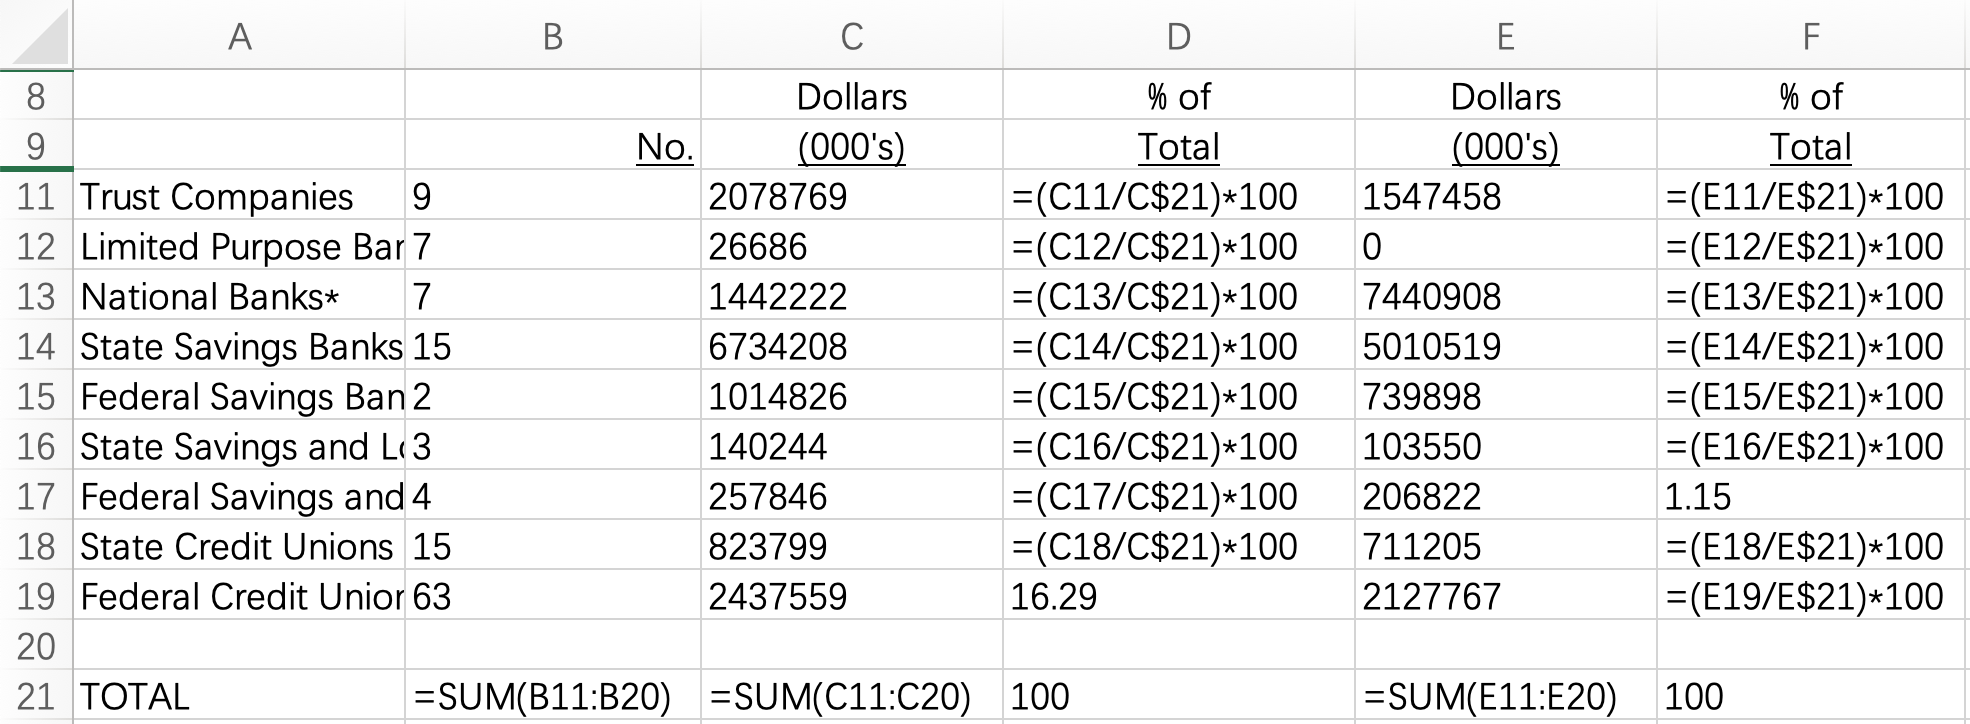
\includegraphics[width=\textwidth]{figure/style-A1.png}
    \caption{截取自EUSES 数据库中的电子表格 summ0602.xls 的工作表summary1201(A1 表示法)}
    \label{figure-A1}
\end{figure}

如图 \ref{figure-A1} 所示,该电子表格显示引用的方式是 A1 表示法。
在 A1 表示法中,一个在第 $X$ 列(A,B,\dots,Z,AA,\dots)第 $y$ 行(1,2,\dots)的单元格在行列都是相对引用的情况下表示为 $Xy$(如B5),在行列都是绝对引用的情况下中表示为 $\$X\$y$(如\$B\$5)。

\begin{figure}[tbp]    
    \centering
    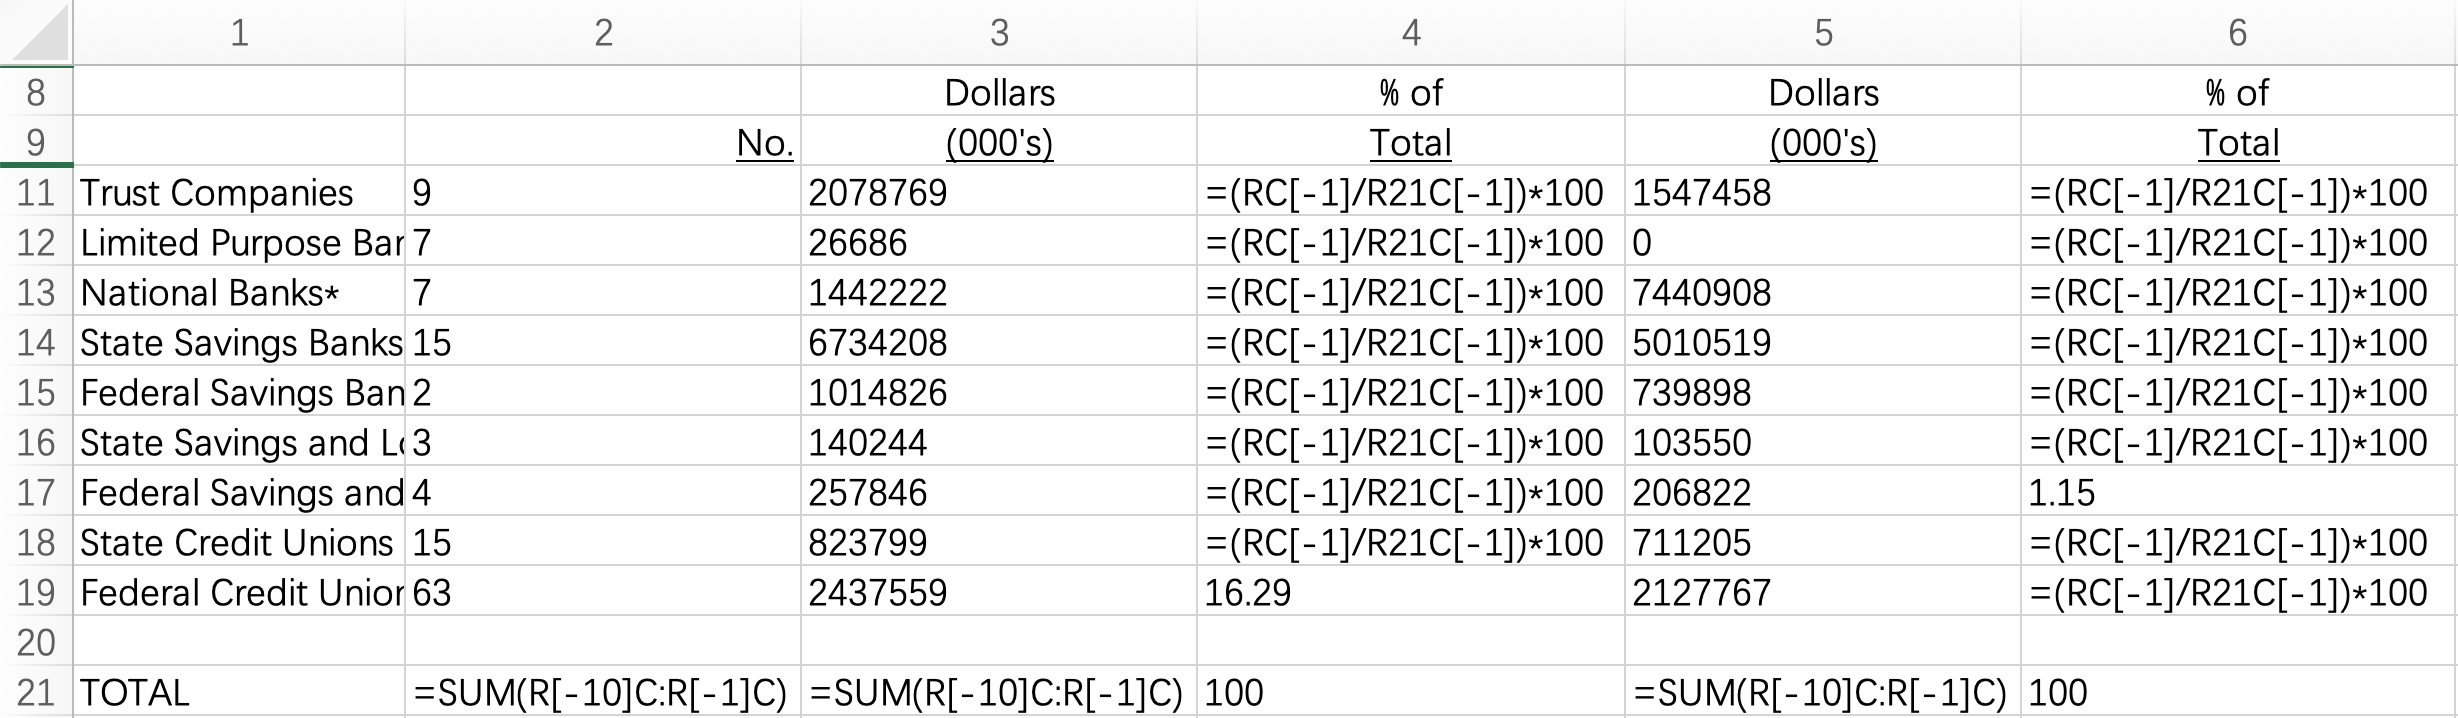
\includegraphics[width=\textwidth]{figure/style-R1C1.png}
    \caption{截取自EUSES 数据库中的电子表格 summ0602.xls 的工作表summary1201(R1C1 表示法)}
    \label{figure-R1C1}
\end{figure}

如图 \ref{figure-R1C1} 所示,该电子表格使用 R1C1 表示法,且所有单元格引用都是相对引用。
在 R1C1 表示法中,一个在当前单元格的下方第 $n$ 行(可以是负数,此时表示上方第 $n$ 行)和右侧第 $m$ 列(可以是负数,此时表示左侧第 $m$ 列)的单元格在行列都是相对引用的情况下中表示为 R[$n$]C[$m$](其中,$n$ 或 $m$ 在 $n=0$ 或 $m=0$ 时可以省略,而一个处在第 $n$ 行,第 $m$ 列的单元格在行列都是绝对引用的情况下表示为 R$n$C$m$。

如图 \ref{figure-A1} 和图 \ref{figure-R1C1} 所示,其中的单元格 D11 就是绝对引用和相对引用混合使用的例子,可以写成两种不同表示形式,即 =(C11$/$C\$21)$*$100 和 =(RC[-1]$/$R21C[-1])$*$100。

我们定义获取一个公式的所有引用的函数 $\sigma(exp)$ ,它返回一个集合,其中包含在该公式中使用到的所有引用。
该函数 $\sigma(exp)$ 可以形式化地表达为:
\begin{definition}
$
\sigma(exp) = 
\left\{
    \begin{aligned}
       & \emptyset & exp \in V; \\
       & \{exp\}     & exp \in R; \\
       & \sigma(exp_1) \cup \dots \cup \sigma(exp_n) & exp = \varphi(exp_1, \dots , exp_n).
    \end{aligned}
\right.
$
\end{definition}

一个有用的观察是:含有相似计算语义的公式单元格通常具有用 R1C1 方式表达的等价表达式。
例如,图 \ref{figure-A1} 中的单元格 D11 中的公式 =(C11$/$C\$21)$*$100 在 R1C1表示法中是图 \ref{figure-R1C1} 中的 =(RC[-1]$/$R21C[-1])$*$100。
图 \ref{figure-R1C1} 也给出了图 \ref{figure-A1} 中其他所有公式对应的 R1C1 表示结果。
我们不难观察出:在 A1 表示法下,从 D11 到 D18 的公式表达式不尽相同,但在 R1C1 表示法下,从 D11 到 D18 的公式表达式完全等价,因此在算法分析和设计时使用后一种表示法更为有利。
我们利用这一观察,从公式表达式中抽取特征来将单元格进行区分,将形式类似的公式吸纳进同一个类中,进而检测出该类中存在的缺陷单元格。


\section{电子表格的缺陷分类}
1997 年,Fowler等人\cite{fowler1997refactoring}提出代码缺陷(Code Smell)的概念。
代码缺陷指导致现有软件中存在潜在的维护问题的不良编码方式。
通常代码缺陷不会立即导致程序错误,但可能显著影响软件的可理解性和可维护性,例如在面向对象程序中,一个冗长的类定义可能难以理解和维护。
从电子表格缺陷的相关研究工作来看,后续的电子表格缺陷定义和分类都明显受到了代码缺陷概念的影响,下面详细介绍。

\subsection{所有类型单元格的缺陷粗分类}
2012 年,Cunha 等人\cite{cunha2012towards}受到代码缺陷的概念启发,率先较为全面地给出了电子表格缺陷的定义以及朴素的识别方法。
他们结合 EUSES 电子表格数据库中的实际案例,对电子表格中可能出现的单元格缺陷进行了分类整理和描述。
他们将电子表格的单元格缺陷分成如下四类:

\textbf{统计相关的缺陷}:
这类缺陷指的是在一列或一行纯数值中,那些不满足正态分布的数值单元格。
这类缺陷通常会引入用户疏忽导致的错误数值。
具体检测思路是计算某行或某列中所有数值的正态分布图,并将正态分布图的 95\% 以外的数值标记为有缺陷的单元格,并报告给用户。
在这类缺陷中,不考虑那些数值或者字符串单元格。
如图\ref{figure-valuesmell}所示,列 B 标准方差是 2.369E8。
那么,被正态分布接受的值应当在 [5.868E8, 1.534E9] 的范围内。
因为单元格 B4 保存着数值 123,这意味着它有可能是有缺陷的单元格。
同理,单元格 G12 也是存在缺陷的。

\textbf{类型相关的缺陷}:
在电子表格中含有四类基本类型的单元格:数值、公式、字符串和空单元格。
通过检查某个特定单元格周围的单元格类型趋势来判断当前单元格是否具有类型不一致性的缺陷。
比较朴素的方法是利用滑动窗口的方式,每次选择某行或某列的连续若干个单元格,检测出该窗口中具有明显与其他单元格具有不同类型的单元格,将其标记为有缺陷的。
如图\ref{figure-valuesmell}所示,我们可以观察到单元格 C6 和 G16 都是空单元格。
然而,它们出现的上下文环境中(这里假设检验时选定的滑动窗口大小为 5)所有的单元格都是被填充的,具有非空类型。
那么,我们即可将这两个单元格标记为有缺陷的。
同理,在单元格 F3 中含有字符串值“o”,但它周围的上下文环境表明列 F 绝大多数单元格都是数值类型,那么单元格 F3 就可以被标记为有缺陷的,其真实值很可能是数值 “0”。

\begin{figure}[tbp]    
    \centering
    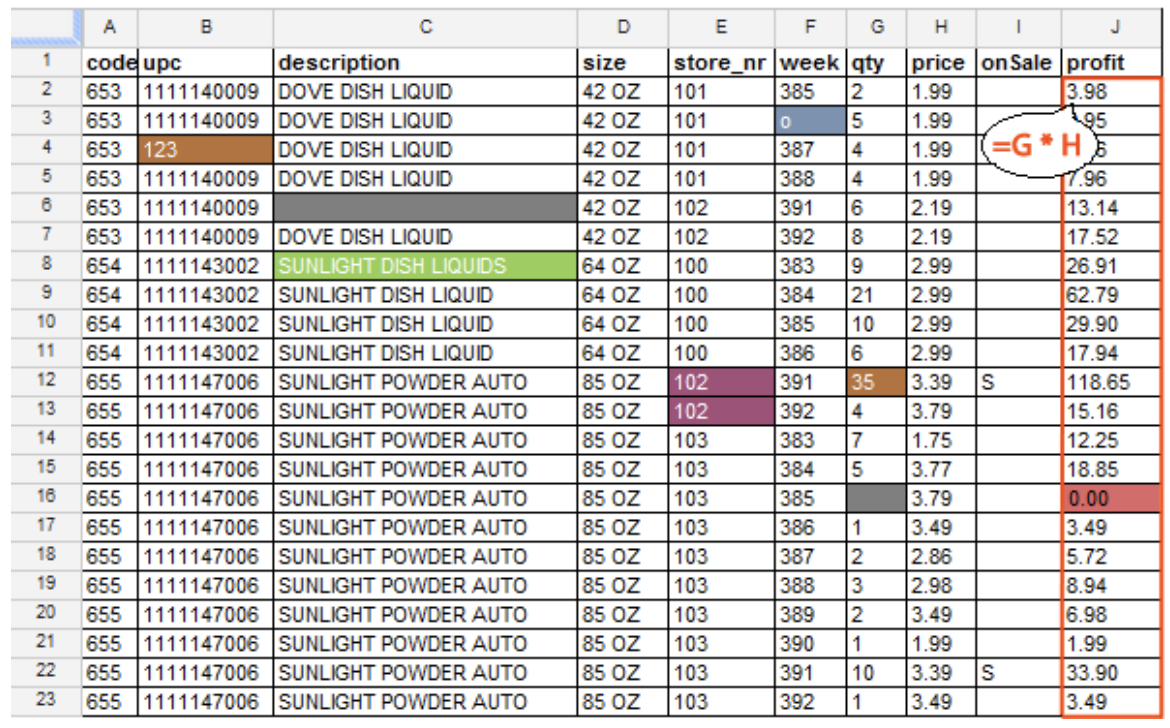
\includegraphics[width=\textwidth]{figure/relatedwork/valueSmell.png}
    \caption{电子表格中的缺陷示意图(其中有缺陷的单元格已用背景色标注出来)}
    \label{figure-valuesmell}
\end{figure}

\textbf{内容相关的缺陷}:
在此类别中,我们通过分析单元格的内容来检测缺陷。
在电子表格的使用环境中,终端用户很容易出现打字错误,比如对于字符串单元格来说,打错、多打、少打了一个字母,都很有可能发生。
我们通过计算两个字符串单元格内容之间的字符串距离,可以来判断是否某个字符串单元格是有缺陷的。
在检测缺陷时,我们可以使用 Levenshtein 算法来进行字符串编辑距离的计算。
如图\ref{figure-valuesmell}所示,单元格 C8 具有单元格 C9 到 C11 的内容的复数形式,而 C8 显然和这些邻近的单元格都有微小的字符串差异,因此我们可以推测该单元格是有缺陷的。

公式单元格也可能具有和内容相关的缺陷,比如该单元格公式引用了空单元格,通常就会导致计算结果无意义。
如图\ref{figure-valuesmell}所示,单元格 J16 被认定为是有缺陷的,因为它引用了空单元格 G16。

\textbf{功能依赖相关的缺陷}:
在此类别中,我们采用数据挖掘技术来检测电子表格中的“脏值”。
检测脏值的方法起初广泛地运用于数据库领域。
这里我们举例说明,如果列 A 中的相同值总是对应着列 B 中的相同值,那么我们说列 A 和列 B 是功能依赖的。
如图\ref{figure-valuesmell}所示,除去少量数据的不满足,列 B 就是功能依赖来列 A,特定的“code”值总是对应于它相应的“upc”值。
当我们检测到在确定已经存在功能依赖的两个列中存在不满足功能依赖的少量单元格时,这些单元格就应当被标记为有缺陷的。
比如单元格 E12 和 E13 被检测为有缺陷的。
因为我们可以发现 在列 A 到列 F元组(655,1111147006,SUNLIGHT POWDER AUTO,85 OZ) 大多数情况下总是对应于列 E 中的值 103,除了 E12 和 E13 不满足。

\subsection{公式类型单元格的缺陷细分类}
2012 年,同样受代码缺陷的启发,但与 Cunha 等人\cite{cunha2012towards}提出的针对所有单元格类型的单元格缺陷定义不同的是,Hermans 等人\cite{hermans2012detecting2,jansen2015code}提出了专门针对公式单元格缺陷的更细粒度的定义。

Hermans 等人结合 EUSES 电子表格数据库\cite{fisher2005euses}的实证经验,提出了五种与公式相关的缺陷种类:

\textbf{过多操作符的缺陷}:
受代码缺陷中“长方法”缺陷\cite{fowler1997refactoring}启发,此类的电子表格公式缺陷与公式的长度(或者说,操作符数量)有关。
它衡量一个公式中包含的操作总量。
图\ref{figure-multipleOperation}展示了一个 EUSES 数据库中具有此类缺陷的公式,它在一个公式内拥有 15 个不同的操作符,对于普通用户来讲很那理解,更加难以进行维护。

\begin{figure}[tbp]    
    \centering
    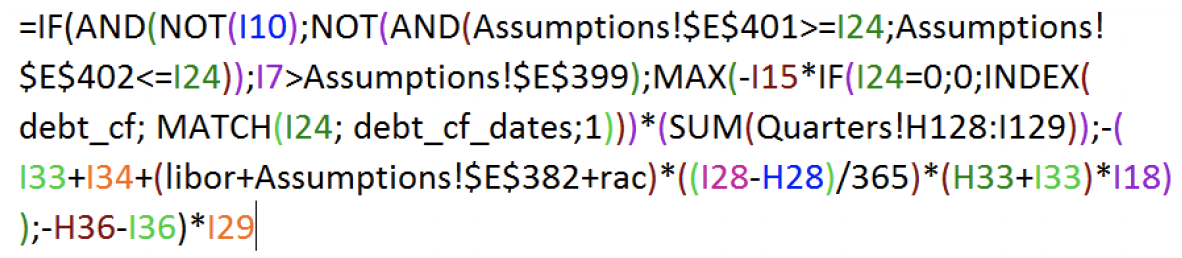
\includegraphics[width=0.8\textwidth]{figure/relatedwork/multipleOperation.png}
    \caption{过多操作符的公式缺陷示例}
    \label{figure-multipleOperation}
\end{figure}

\textbf{过多引用的缺陷}:
另一类臭名昭著的代码缺陷是方法定义拥有过多参数。
与此类似,在电子表格公式中就对应于过多单元格引用。
此类缺陷统计公式中引用的单元格数量。
图\ref{figure-multipleReference}展示了一个 EUSES 数据库中具有此类缺陷的公式,它总共含有 79 个单元格引用,显然给用户理解和维护带来困难。

\begin{figure}[tbp]    
    \centering
    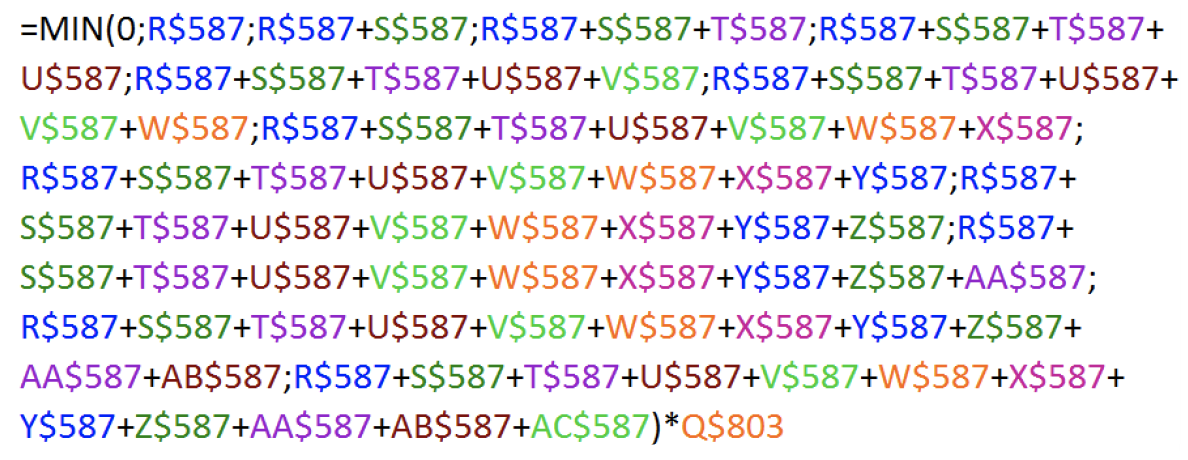
\includegraphics[width=0.8\textwidth]{figure/relatedwork/multipleReference.png}
    \caption{过多引用的公式缺陷示例}
    \label{figure-multipleReference}
\end{figure}

\textbf{过多条件嵌套的缺陷}:
过度嵌套的条件判断被认为是代码可读性的威胁\cite{fowler1997refactoring}。
对于电子表格公式来说,过多条件嵌套也影响了公式的可读性。
此类缺陷统计公式中条件嵌套的数量。
图\ref{figure-ConditionalComplexity}展示了 EUSES 数据库中的一个有 7 层嵌套的 IF 公式,Excel 2003 版本 最多只允许 7 层 IF 嵌套,这显然也有碍于电子表格的长期维护。

\begin{figure}[tbp]    
    \centering
    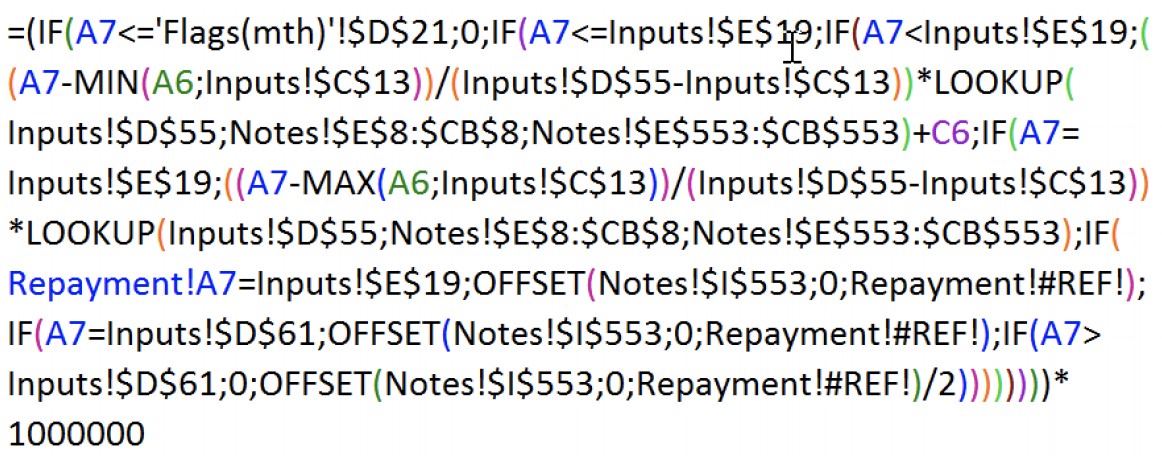
\includegraphics[width=0.8\textwidth]{figure/relatedwork/ConditionalComplexity.png}
    \caption{条件过度复杂的公式缺陷示例}
    \label{figure-ConditionalComplexity}
\end{figure}

\textbf{过长计算链的缺陷}:
电子表格中,公式引用很常见,因此这些引用关系就构成了电子表格的计算链。
追踪一个过长计算链对用户来说是一项枯燥且易错的任务。
此类缺陷通过衡量计算一个公式所需最长的引用路径长度。

\textbf{重复公式的缺陷}:
在代码维护中,我们通常想要同构的代码片段只有一份,方便日后的修改和维护。
同样地,电子表格中的公式也可能存在这样的问题。
如某个单元格中的公式是另一个公式的子公式,那这个单元格就被成为具有重复公式的缺陷。
通过对比R1C1表示法下的各个公式语法树,来判断是否存在此类缺陷。
如图\ref{figure-DuplicatedFormula}所示,第 39 行的四个公式具有完全相同的公式,因此这四个公式都具有重复公式的缺陷,
我们可以保留其中一个公式,另外三个直接引用被保留公式的计算结果即可,避免了维护的复杂性。

\begin{figure}[tbp]    
    \centering
    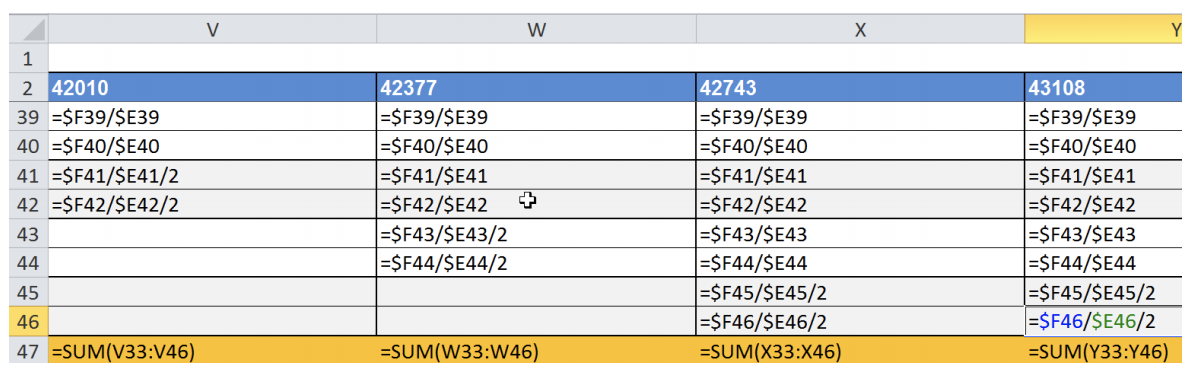
\includegraphics[width=\textwidth]{figure/relatedwork/DuplicatedFormula.png}
    \caption{重复公式的公式缺陷示例}
    \label{figure-DuplicatedFormula}
\end{figure}

\subsection{小结}
得益于 Cunha 和 Hermans 等人踏实的实证研究工作和缺陷分类整理\cite{cunha2012towards,hermans2012detecting2,jansen2015code},很多后续的缺陷预防和检测相关技术都是针对其中某些缺陷,提出行之有效的技术思路和实现方法。
在后续的相关工作中,研究者们也对缺陷定义做了各种细化和延伸的工作,但其基本骨架已经被这两种分类方式搭建起来,没有经历大的变化。


\section{电子表格缺陷的相关工作}
从电子表格的缺陷引入过程中,其本身就可以分成在缺陷引入前的技术研究(即缺陷预防)以及在缺陷引入后的技术研究(即缺陷检测和修复)两方面。
限于篇幅有限,本节分两小节分别讨论模型驱动相关的缺陷预防技术和各种类型的缺陷检测技术(本文的技术就属于后者),因为这两个技术方向在电子表格领域影响力较为深远,且相关工作众多。
电子表格的公式本身虽然可能很复杂,但其所属的缺陷类型对于终端用户来说,一经指出,就不难理解,因此终端用户通常也能进行相对快速的手工缺陷修复,因此本文不再专门讨论缺陷修复相关的技术研究,此部分可以参考其它综述文章\cite{jannach2014avoiding}。

\subsection{电子表格的缺陷预防}
%------
1995年,Isakowitz 等人\cite{isakowitz1995toward}开始提出对电子表格中的数据及其结构进行建模。
他们把电子表格看做物理和逻辑的两个部分,物理部分就是单元格的公式和数值,逻辑部分就是描述电子表格功能的一系列函数关系。
借用他们设计的函数式关系型语言,通过提取算法能够从电子表格中将单元格之间的计算关系提取出来;类似地,也可以通过该关系型语言描述的电子表格模型生成实际的电子表格,即实现了从具体电子表格数据到模型之间的互相转换。
该工作为后续将面向对象技术和模型控制技术向电子表格的应用,奠定了基础。

1997年,Paine 等人\cite{ireson1997model,paine2008ensuring,paine2005bringing,paine2008rapid}也提出了针对电子表格的面向对象概念。
在他们的 Model Master 方法中,电子表格以声明式的方式表达为文本程序。
这些程序通过编译器处理,随即从规约中生成电子表格。
电子表格的数值和计算逻辑以类的形式表达,其中包括属性和相应的计算逻辑。
2008年,Paine等人\cite{paine2008spreadsheet}在之前Model Master工作的基础上,进而提出了针对电子表格的“结构发现”技术,使用编程语言Prolog来限定电子表格可能的逻辑结构。
该方法的目标是作为电子表格软件的“智能结构监控器”,允许用户在编辑表格的同时对表格结构进行重配置。
原作者们认为该技术可能是电子表格“最佳实践”的革命性成果。

\begin{figure}[tp]    
    \centering
    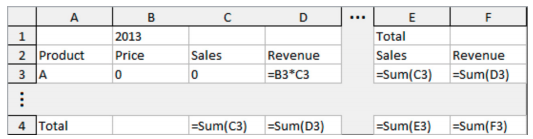
\includegraphics[width=1\textwidth]{figure/template.png}
    \caption{电子表格模板示例}
    \label{figure-template}
\end{figure}



%  2004年,Erwig等人\cite{erwig2004gencel,erwig2005automatic,abraham2005goal}提出基于表格模板的可视化方法来刻画电子表格底层模型的特定方面。
%  在他们的 Gencel 方法中,一个“表格模板”被用来特指电子表格中重复的区域。
%  模板的设计和修改过程类似于 MS Excel 软件的可视化操作方式。
%  图\ref{figure-template}展示了一个可视化模板的例子,其中列B、C和D下面的内容被标记为可重复的。
%  这类可重复的区域用所在列上和所在行上的两个省略号"..."和两条分隔带来表达。
%  2006年,Abraham等人\cite{abraham2006inferring}提出使用一些启发式方法能够从给定的电子表格中自动提取出存在的模板。

2010年,后来,Engels等人\cite{engels2005classsheets,cunha2010automatically}结合基于模板的方法和面向对象的概念模型提出了 ClassSheet 的概念,
突破了基于模板方法只能刻画电子表格的“词法特征”的局限性,使用 ClassSheet 概念能够更完整地刻画整个表格的“语义特征”。
许多基于 ClassSheet 概念的改进方法被陆续提出\cite{luckey2012systematic,cunha2011type,cunha2011embedding,cunha2012bidirectional}。
比如 Luckey等人\cite{luckey2012systematic}处理了模型演化和如何使得这类更新能够自动转换到已经生成的电子表格中的问题,以便更好地支撑电子表格完整的开发过程。

同年,Hermans等人\cite{hermans2010automatically}提出了另一个不同的可视化方法来重构底层面向对象模型。
该方法基于人工设计的经典模式库,通过二维解析和模式匹配算法来尝试定位电子表格中的各类构建模式。
最终的构建模式被转换成 UML 类图,可用于更好地理解和提升当前的电子表格质量。


\subsection{电子表格的缺陷检测}
本世纪的前 10 年主要的缺陷检测相关工作,关注于使用类型推导的方法\cite{erwig2002adding,burnett2002testing,ahmad2003type,abraham2004header,abraham2006type,abraham2007ucheck,antoniu2004validating,chambers2009automatic,chambers2010reasoning}来检测电子表格缺陷。
这类方法的核心思路是借助人工标注或者字符串信息推导出数值单元格的类型信息,进而判断公式中的计算是否符合不同类型之间的运算法则,类似于传统程序在编译器中进行的静态类型检查。

Erwig等人\cite{erwig2002adding,abraham2004header,chambers2009automatic}最早把这种类型推导系统引入到电子表格的特定错误检测中来。
他们依据表头来推导类型信息,并结合用户标注的类型信息,推导出所有可能的数值单元格类型,进而验证公式运算的类型合法性。
但该方法需要较多的额外信息输入,才能分析出数值单元格的类型,对很多商用电子表格并不适用,因此适用范围较小,能够检测出的缺陷类型也相对较少。

本世纪的 20 年代至今,研究者们更加关注电子表格中与公式相关的缺陷。
这些电子表格公式缺陷本身未必是错误的,但在未来的软件开发、重构或拓展过程中可能导致错误。

正如本章第二节所述,Hermans 等人\cite{hermans2012detecting,hermans2012detecting2,hermans2013data}率先关注此类公式缺陷。
2012年,Hermans等人\cite{hermans2012detecting2}率先将代码缺陷概念移植到电子表格领域,针对公式类型单元格定义了五种相关缺陷。
该方法通过一系列的硬性统计指标来衡量一个公式单元格是否有缺陷,并将有缺陷的部分在电子表格中高亮出来,供用户进一步分析。
同年,Hermans等人\cite{hermans2012detecting}使用类似于\cite{hermans2012detecting2}的思路考察跨工作表之间(inter-worksheet),但表格结构相似的对应单元格中是否有缺陷。
次年,Hermans等人\cite{hermans2013data}基于现有的文本克隆检测算法,适配到电子表格中,检测公式之间的复制-粘贴关系,识别出那些在复制公式时仅复制值的电子表格缺陷(因为仅复制公式的值会导致后续可读性和维护性显著恶化)。

2014年,窦文生等人\cite{dou2014spreadsheet}注意到具有相同计算语义的电子表格单元格在布局上常常是连续的多个单元格,并且同属于相同的行或列\footnote{类似于用一个矩形圈出的单列或单行连续多个单元格区域,称为\textit{单元格阵列}(\textit{cell array})}。
在表格演化的过程中,由于特定的修改或者破坏性的复制-粘贴操作,单元格这列中的单元格不再具有相同的计算语义,那么该单元格阵列中就含有有缺陷的单元格了。
该技术AmCheck使用启发式的方法,结合公式引用的同构特性,来识别这些单元格阵列区域,进而使用启发式策略和程序合成技术来检测并修复每个单元格阵列中的单元格缺陷。
2016年,窦文生等人\cite{dou2016detecting}将关注的目光放到克隆的表格上\footnote{这里的表格(table)指一个多行多列的矩形区域,包含字符串表头,以及多个核心的数值和公式单元格,如果把工作表比作一个Java类,那么表格就是其中一个方法,用以实现某个特定功能}。
在克隆的表格之间的对应单元格理应保持相同或相似的计算语义。然而,和\cite{dou2014spreadsheet}中指出的相似原因,克隆的表中会存在有缺陷的单元格。
该技术TableCheck根据表头信息和已有的基于指纹概念的代码克隆检测技术来判断两个表格是否是克隆关系,一经确定,进而使用启发式策略来判断每个单元格是否保持了相同的语义,其中的异常者就是有缺陷的单元格,终端用户可以参考克隆表格的信息来修改检测出的缺陷。
2017年,窦文生等人\cite{dou2017cacheck}在 \am 技术的基础上进行实证研究,发现除了同构类型的单元格阵列之外,另一类具有异构特性的单元格这列在EUSES数据集中也频繁出现,因此他们提出CACheck技术能够同时识别出同构和异构的单元格阵列,并利用和 \am 相似的技术进行后续的缺陷检测和修复推荐。
2018年,Xu等人\cite{xu2018spreadsheet}对电子表格模板在真实商业数据集Enron上的使用进行实证研究。
他们发现终端用户由于缺陷必要的工具支撑,难以找到预先定义好的表格模板,通常选择从已有表格中进行表格克隆,然后进行修改,这样不可避免地导致发生在一个表格中的缺陷不断衍生下去。
2020年,Zhang等人\cite{zhang2020learning}在TableCheck技术的基础上进行实证研究,发现超过一半的发生克隆的表格中发生了结构变化,比如新增了几行或者几列数据,然而TableCheck技术只能检测结构相同的克隆表格。
该技术LTC通过提取通常保持相似的结构和格式,比如表头,公式和背景颜色等信息,来构造二分类器,进而识别出带有结构变化的克隆表格。
实验表明,LTC技术相比TableCheck取得了精度和召回率上的极大提升。
本文在实验评估部分,选用了\am 和 \ca 这两个缺陷检测技术作为我们\wa 技术的对比技术,因为这两个技术在使用模式匹配和设计精妙的启发式方法来辅助识别单元格阵列和公式缺陷方面效果显著,是主流的缺陷检测技术之二。

2016年,Cheung等人\cite{cheung2016custodes}注意到\am 和 \ca 技术只能检测单元格这列这种结构的单元格类,如果具有相似计算语义的单元格不是连续分布,就无法被这两种技术识别出来。
因此,他们提出了 \cu 技术,基于机器学习的两阶段聚类方法来对单元格进行聚类,识别出足够多的单元格类,进而通过离群点检测技术在每个单元格类中识别出离群点,即具有缺陷的单元格。
该方法因为采用特征抽取的方式来进行聚类,克服了单元格类必须连续的局限性,同时也提升了识别单元格类的召回率。
值得一提的是,直到2016年,针对电子表格的公式缺陷设计的基准测试集(采样自EUSES数据库)才得到后续研究工作的广泛使用,有利于后续工作\cite{singh2017melford,Barowy2018excelint}在实验评估中进行有效的技术对比。
本文即是对 \cu 技术的进一步优化,后面的方法设计和实验评估章节都会进一步介绍,此处不再赘述。

\begin{figure}[tbp]    
    \centering
    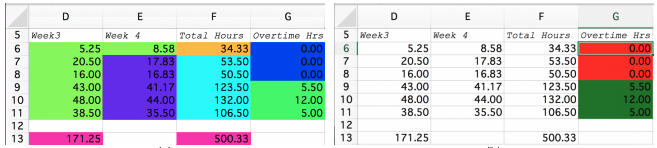
\includegraphics[width=1\textwidth]{figure/figure-excelint.png}
    \caption{ExceLint 工具对公式单元格的划分结果展示}
    \label{figure1}
\end{figure}

2017年,Singh等人\cite{singh2017melford}利用近些年在语音和图像识别领域大火的深度学习技术来检测本该是公式但用纯数值表示的单元格缺陷。
该技术Melford通过对被检测的单元格周围进行单元格的空间抽象来构建分类器,用于判断该单元格是否应该包含一个公式。
该方法理论上能够和 \cu 技术形成互补,不过目前的实验表明该方法能够检测出的缺陷数量仅是\cu 的子集,但原作者认为即便使用了简单的深度学习训练模型,已经取得了不俗的效果,表明该技术方向有广阔的应用前景。

2018年,Barowy等人\cite{Barowy2018excelint}采用信息论的方法来检测公式相关的缺陷。
该方法充分利用电子表格的矩形特征,根据信息熵的计算结果来识别最能显著破坏矩形区域的公式,利用这些有突出代表性的公式来对整个表格进行矩形切分,如图\ref{figure-excelint}所示。
最终,在每个识别出的矩形区域,每个公式单元格应当具备相似的计算语义,进而根据单元格引用特征来识别出离群点,即那些有公式引用缺陷的单元格。
此技术ExceLint在实验中\cite{Barowy2018excelint}与\cu 技术进行对比,在检测公式引用缺陷方面比\cu 取得了更好的效果。

2019年,Koch等人\cite{koch2019refinement}发现当前已有的电子表格缺陷检测技术具有几个共同的缺陷,导致不正确的或冗余的缺陷报告。
例如,相同的质量问题经常在每个单元格的克隆副本上都被汇报出来,这巨大的缺陷数量可能使得终端用户难以承受。
因此,Koch等人提出对检测出的电子表格缺陷进行进一步筛选再汇报给终端用户,通过使用在缺陷检测阶段推导出的结构化信息。
该方法在实验中也证实了能够显著减少不正确的和冗余的缺陷报告。

\subsection{小结}
%这里还是要再引用10篇左右近三年的论文,不能胡扯
除了直接针对电子表格的缺陷检测技术,近些年研究者们也在考虑如何自动化地从不同的角度帮助终端用户来提升电子表格的可靠性和可维护性。

比如,Zhang等人\cite{zhang2018automated}就重点关注我们在第2.2.2节提到的多层嵌套IF公式的自动化重构技术。
另外,Xu等人\cite{xu2018detecting}关注于如何检测有缺陷的空单元格,接近于我们在第2.2.1节提到的本该有公式却只是一个空单元格的类型相关的缺陷。



% 电子表格的相关工作主要集中在两个研究领域,信息系统和计算机科学领域。
% 在本章中,我们从计算机科学领域(主要是软件工程)的视角出发,对电子表格的质量保障技术进行分类讨论。
% 根据它们的设计目的,我们把各种电子表格的质量保障技术分成两类:
% \begin{itemize}
    % \item \textit{避免错误}的技术帮助终端用户从开发的起始阶段就能创建出不含错误的电子表格,对应本章第一节讨论的相关工作;
    % \item \textit{发现和修复错误}的技术帮助终端用户检测电子表格中蕴含的错误并理解错误发生的原因,进而修复这些的错误。
    % 这类技术通常在电子表格已经开发、编辑完成之后使用,对应本章第二节和第三节讨论的相关工作。
% \end{itemize}

% 接下来,我们将相关工作分成三个小节来讨论,即模型驱动的电子表格开发技术、电子表格的缺陷定位、检测和修复技术、以及电子表格的辅助支撑技术。

%  \section{模型驱动的电子表格开发技术}
%  基于模型驱动的方法并不是设计用来帮助终端用户发现潜在的错误,而是把提升电子表格的质量、结构的清晰度和防止错误注入放在首位。
%  类似于一般软件工程领域的模型驱动方法,这类技术的核心想法是在电子表格的开发过程中引入额外的抽象层。
%  这个额外的抽象层引入了更多抽象概念,在开发者的内在意图和电子表格的真实实现中间充当了沟通的桥梁。
%  在商业化的电子表格系统中日益扩大的这层语义鸿沟\cite{luckey2012systematic}得到了有效缓解。

%  这类抽象的电子表格模型通常出现在开发过程的两个阶段:
%  \begin{itemize}
    %  \item 它们被用作“代码生成器”的形式化描述。在这个场景下,电子表格的一部分从模型中自动生成,因此减少了纯人工操作产生错误的风险;
    %  \item 它们也被用于从已有的电子表格中恢复出内在蕴含的概念结构,帮助终端用户理解当前电子表格的计算模型,进而减少后续可能产生的误解。
%  \end{itemize}

%  \subsection{电子表格的面向对象模型}
%  Isakowitz 等人\cite{isakowitz1995toward}是最早提出从建模角度来处理电子表格程序。
%  他们的核心假设是电子表格程序可以看做物理和逻辑的两个部分,物理部分就是单元格的公式和数值,逻辑部分就是描述电子表格功能的一系列函数关系。
%  而逻辑这部分可以从给定的电子表格中自动提取出来,并用领域特定语言(Domain-specific Language,DSL)表达出来。
%  该系统也能够从这样的逻辑规约中合成电子表格。

%  Paine 等人\cite{ireson1997model,paine2008ensuring}也提出了类似的针对电子表格程序的面向对象概念。
%  在他们的 Model Master 方法中,电子表格以声明式的方式表达为文本程序。
%  这些程序通过编译器处理,随即从规约中生成电子表格。
%  电子表格的逻辑以类的形式表达,其中包括属性和计算逻辑。
%  该建模语言中也提供许多特征(如类继承,多维数组扩展)来支持表格化的计算。
%  我们也可以逆向使用该方法,从给定的电子表格中提取出对应的逻辑模型,进而用于发现电子表格中的特定计算结构\cite{paine2008spreadsheet}。

%  Paine 等人\cite{paine2005bringing,paine2008rapid}后续提出了另一种声明式建模语言。
%  他们开发的 Excelsior 是一个电子表格开发系统,构建在 Prolog 上的编程语言,同时针对 Excel 设计了模块化和可重用的规约表达方式。

%  \begin{figure}[tp]    
    \centering
    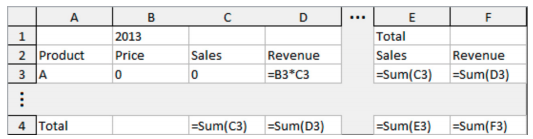
\includegraphics[width=1\textwidth]{figure/template.png}
    \caption{电子表格模板示例}
    \label{figure-template}
\end{figure}
%  \subsection{电子表格的可视化模板}
%  Erwig 等人\cite{erwig2004gencel,erwig2005automatic,abraham2005goal}提出基于表格模板的可视化方法来刻画电子表格底层模型的特定方面。
%  在他们的 Gencel 方法中,一个“表格模板”被用来特指电子表格中重复的区域。
%  图\ref{figure-template}展示了一个可视化模板的例子。
%  模板的设计和修改过程类似于 MS Excel 软件的可视化操作方式。
%  在图\ref{figure-template}中,$B$、$C$和$D$列下面的内容被标记为可重复的。
%  这类可重复的区域用所在列上和所在行上的两个省略号"..."和两条分隔带来表达。

%  类似于 Paine 等人的工作,电子表格也可以从模型中自动生成。
%  另外,基于模板的方法也支持逆向工程,Abraham 等人\cite{abraham2006inferring}提出使用一些启发式方法能够从给定的电子表格中自动提取出存在的模板。

%  后来,Engels 等人\cite{engels2005classsheets,cunha2010automatically}结合基于模板的方法和面向对象的概念模型提出了 ClassSheet 的概念,
%  突破了基于模板方法只能刻画电子表格的“词法特征”的局限性,使用 ClassSheet 概念能够更完整地刻画整个表格的“语义特征”。
%  许多基于 ClassSheet 概念的改进方法被陆续提出\cite{luckey2012systematic,cunha2011type,cunha2011embedding,cunha2012bidirectional}。
%  比如 Luckey 等人\cite{luckey2012systematic}处理了模型演化和如何使得这类更新能够自动转换到已经生成的电子表格中的问题,以便更好地支撑电子表格完整的开发过程。

%  Hermans等人\cite{hermans2010automatically}提出了另一个不同的可视化方法来重构底层面向对象模型。
%  该方法基于人工设计的经典模式库,通过二维解析和模式匹配算法来尝试定位电子表格中的各类构建模式。
%  最终的构建模式被转换成 UML 类图,可用于更好地理解和提升当前的电子表格质量。

%  \subsection{电子表格的关系型模型}
%  电子表格的主要原则之一:数据以表格的形式组织。
%  一个直接的获得表格的结构模型的方法是借鉴关系型数据库的设计原理和实践方法。
%  以构建高质量和零错误的表格为目的,Cunha 等人\cite{cunha2009spreadsheets}提出了从电子表格中提取关系型数据库范式的方法。
%  该方法的主要优点是能够获得更加模块化、没有数据冗余、并预防错误的数据输入的电子表格模型\cite{cunha2009discovery,cunha2012relational}。


%  \section{电子表格的缺陷分析技术}
%  电子表格的编程范式使得终端用户容易犯错。
%  随着电子表格包含的数据量越来越大,依赖终端用户人工检查每个公式的计算结果是否符合预期,效率低下。
%  相应地,针对电子表格的自动化错误/缺陷定位、检测和修复工作得到了研究者们的广泛关注。
%  这些方法也可以基于是否需要人工辅助分成两类,人工辅助具体包括用户给定测试输入、按要求提供额外的标注信息等。

%  \subsection{缺陷定位}
%  早期的电子表格错误定位工作\cite{reichwein1999slicing,ruthruff2005interactive},使用计算轨迹的候选者排序策略来寻找有缺陷的单元格,类似于传统程序分析中的基于频谱的错误定位方法。
%  他们首先提出将程序切片的概念应用到电子表格中,以消除不可能的错误候选者。
%  该类技术使用用户给定的辅助信息关于正确和不正确的单元格值,并把对一个错误的单元格值有贡献的单元格标记为可能错误的。
%  一个单元格的公式如果对更多的已经标记为错误的值有贡献,那么很可能就是错误的。
%  相反,对更多正确的单元格值有贡献,那么很可能就是正确的。
%  如果一个单元格对错误的单元格值有贡献,但是它本身只由正确的单元格值计算而来,那么它的错误可能性就会减小。
%  该类方法,就是依据这种想法,进行量化排序。
%  后续,Hofer 等人\cite{hofer2013empirical}使用更加形式化的方法,以相似性系数来计算电子表格单元格的错误可能性。

%  另一条错误定位的思路是把电子表格转换成基于约束的形式,使得关于异常值的原因定位的复杂推导变得可能。
%  Jannach 等人\cite{jannach2010toward}提出将电子表格错误定位问题转换成约束可满足性问题(CSP)\cite{tsang2014foundations}。
%  基于用户给出的测试用例和关于某些单元格的异常值信息,该方法使用基于模型诊断的原则来判定哪些单元格原则上可能是异常计算结果的真正原因。
%  后来,Jannach 等人\cite{jannach2016model}又提出了新的算法改进策略,帮助提升原方法的可扩展性。

%  类似的方法也得到了 Abreu 等人\cite{abreu2012constraint,abreu2012debugging}的采用。
%  Abreu 的方法尽管整体上与 Jannach 等人的方法相似,但技术实现上有差异。
%  他们没有使用 Hitting-Set 算法\cite{reiter1987theory},而是把单个公式的正确性的推导直接编码成约束表达。
%  因此他们利用了额外的布尔变量来代表每个公式的正确性。
%  另外他们的方法可以同时运用于多组测试用例的并发执行。

%  Hofer 等人\cite{hofer2013empirical}提出把一个轻量级的基于模型的调试技术,结合到他们的基于频谱的错误定位方法中。
%  他们建议使用从统计错误定位技术(SFL)得到的系数作为基于模型的调试过程的初始可能性值。

%  \subsection{缺陷检测}
%  本世纪的前 10 年主要的缺陷检测相关工作,关注于单位和类型推导的方法\cite{erwig2002adding,burnett2002testing,ahmad2003type,abraham2004header,abraham2006type,abraham2007ucheck,antoniu2004validating,chambers2009automatic,chambers2010reasoning}来检测电子表格错误或缺陷。
%  这类方法的核心想法是推导出输入单元格的单位信息,进而判断公式中的计算是否符合单位之间的运算法则,类似于普通程序在编译器中进行的静态类型检查。
%  Erwig等人\cite{erwig2002adding,abraham2004header}最早把这种单位推导系统引入到电子表格的特定错误检测中来。
%  他们根据表头推导策略和用户标注,推导出所有可能的输入单元格单位信息,进而验证公式的单位运算合法性。

%  本世纪的 20 年代至今,学界更加关注一类称为电子表格缺陷(Spreadsheet Smell/Defect)的公式错误,该概念派生于软件维护领域的代码潜在错误\cite{fowler1997refactoring},用于特指不良代码设计风格和使用习惯。
%  这些代码本身未必是错误的,但在未来的软件开发、重构或拓展过程中可能导致错误。
%  Hermans 等人\cite{hermans2012detecting,hermans2012detecting2,hermans2013data}最早明确地将此类概念发展到电子表格领域中。
%  通常,电子表格缺陷是通过一些启发式的方法来描述不良设计风格。
%  Hermans 等人\cite{hermans2012detecting} 提出所谓的“工作表之间的单元格缺陷”。
%  这类缺陷根据不同工作表之间的依赖关系分析,来识别一些不良使用导致的单元格缺陷。
%  比如,一个公式引用了很多另一个工作表中的单元格,那么该公式应当被移动到对应工作表中。
%  公式缺陷最早在\cite{hermans2012detecting2}的工作中得到较为深入的分类和讨论。
%  后续,Hermans 等人\cite{hermans2013data}提出一个定位电子表格中数据克隆的方法。

%  窦文生等人\cite{dou2014spreadsheet,dou2017cacheck}提出“单元格阵列”的缺陷检测方法,通过定位同行或同列的具有类似公式语义的连续单元格阵列,进而利用基于组件的程序合成方法在每个单元格阵列中来检测公式异常。
%  后来,窦文生等人\cite{dou2016detecting}又提出进行跨表格(table)的克隆检测和单元格缺陷检测,通过识别结构同构的表格,进而对相应位置的单元格进行对比,来寻找公式异常。

%  \begin{figure}[tbp]    
    \centering
    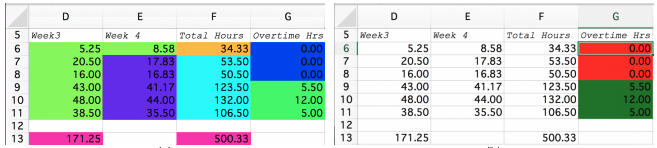
\includegraphics[width=1\textwidth]{figure/figure-excelint.png}
    \caption{ExceLint 工具对公式单元格的划分结果展示}
    \label{figure1}
\end{figure}
%  考虑到前人工作的召回率偏低问题,Cheung等人\cite{cheung2016custodes}提出基于学习和聚类的技术来对单元格进行分类,尽可能保证每个类中的单元格都含有相似的计算语义,进而在类中检测公式缺陷。
%  本文即是对 Cheung 等人工作的进一步优化和提升,后面的章节会进一步介绍。
%  类似地,如图\ref{figure-excelint}所示,ExceLint\cite{Barowy2018excelint}技术通过对公式中蕴含的信息熵分析来给出最合理的电子表格切分方式,最后在每个切分出的单元格矩阵中来进一步检测是否存在公式缺陷。
%  Melford\cite{singh2017melford}技术通过提取每个单元格附近的其他单元格属性,利用神经网络模型来寻找异常单元格,它的检测范围是\cu \cite{cheung2016custodes}的真子集。

%  \subsection{缺陷修复}
%  基于修复的方法不仅向用户指出有潜在问题的公式,也额外给出修复方案,比如应该把错误的公式修改成何种具体的正确公式。
%  Abraham 等人\cite{abraham2005goal}做出了第一份自动化给出修改建议的工作 GoalDebug(以目标为导向的调试技术)。
%  该方法中,需要用户为错误的单元格给出预期的结果,通过递归修改单个公式,根据电子表格特定的修改推导规则反向传播到之前的公式中,进而尝试自动给出合适的修改建议。
%  能够获取预期结果的修改结果再根据启发式方法进行排序。
%  另一个改进上述提到的 GoalDebug 的方法 \cite{abraham2007goaldebug,abraham2008mutation} 更适合处理多种的电子表格错误类型。
%  在缺陷检测中提到的工作\ca \cite{dou2014spreadsheet,dou2017cacheck},通过基于组件的程序合成技术\cite{jha2010oracle}也能够为检测到的单元格缺陷提供基础的修复公式建议。


%  \section{电子表格的辅助支撑技术}
%  这类辅助支撑技术在电子表格的开发和维护过程中给予用户帮助,包括帮助用户避免发生引用错误、
%  对电子表格的长期使用提供支撑(监控表格变动的工具、自动化重构的插件等),以及自动帮助用户完成数据提取任务的程序合成工具。

%  \subsection{演化}
%  电子表格通常经历各种变化,不巧的是,变化常常会引入错误。
%  FormulaDataSleuth\cite{bekenn2008reducing}是一个旨在帮助电子表格开发者在表格变动时,立刻检测到这类错误的工具。
%  一旦开发者已经声明了哪些数据单元格和区域应当被工具监控,系统就会自动监测许多类型的潜在问题。
%  对于已经定义好的数据区域,工具能够检测出空单元格、或者输入值拥有错误的数据类型、或者超出了预定义的数据范围。
%  对于被监控的公式单元格,偶然的公式重写以及引用了错误的单元格也会被识别出来。

%  理解给定的电子表格如何随着时间演化,并观察不同版本之间的差异,对于在不同项目中重用电子表格至关重要。
%  Chambers 等人\cite{chambers2010sheetdiff}提出了 SheetDiff 算法,能够检测并可视化特定类型的不同版本的电子表格之间的显著差异。
%  后来,为了克服上述贪心算法 SheetDiff 中存在的问题,Harutyunyan 等人\cite{harutyunyan2012planted}提出一种基于动态规划的算法 RowColAlign,能够更加高效和准确地检测版本差异。
%  徐良等人\cite{xu2017spreadcluster}利用聚类技术对电子表格整体进行聚类,进而寻找出多个电子表格文件之间的演化关系,并给出了我们在第六章案例研究中使用的测试对象,一个电子表格数据集 VEnron2。

%  \subsection{重构}
%  重构被定义为修改程序内部结构,但不修改功能性的过程\cite{o2010spreadsheet}。
%  除了应用于传统代码,重构在多个方面也有助于电子表格的质量保障。
%  比如,通过简化公式,使得整体更易理解;通过移除冗余公式,使得维护更加轻松,更少犯错。
%  电子表格领域的重构通常和行列调整有关,也就是电子表格的设计和布局的转换。
%  让终端用户人工进行这类转换,常常是耗时且易错的。

%  Badame等人\cite{badame2012refactoring}根据使用经验提出电子表格中的七种重构策略,并给 MS Excel 软件提供了一个相应的重构插件 RefBook。
%  该插件自动检测需要重构的单元格位置,并给终端用户提供重构建议。
%  例如可能提供的重构建议有:将单元格常量化、添加“守护”单元格、以及替换不合理的公式等。

%  Harris等人\cite{harris2011spreadsheet}提出了一种根据用户给定的样例进行复杂表格转换的方法。
%  该方法基于一个描述表格转换的领域特定语言 TableProg,以及一个 ProgFromEx 算法。
%  该算法需要用户提供几组转换示例,描述单元格变化前后的具体字符串。
%  ProgFromEx 能够自动推导出若干个转换程序,选择其中排序最高的一个,来帮助终端用户完成这样的表格转换过程。
%  与此类似的相关工作很多,研究者们将程序合成、程序语言领域的理论成果应用到电子表格的实际使用中,如 FlashFill\cite{singh2016transforming}。

%  \subsection{复用}
%  通常,复用已有的已经验证过的软件制品能够节约开发时间,避免犯错的风险,提升整体项目的可维护性\cite{ye2005reuse}。
%  这种复用思路也可以应用于电子表格领域。
%  独立的电子表格或者其中的部分通常可以在其他项目中重用。
%  对于公式复用的标准做法是简单的复制粘贴该公式。
%  然而,改变最初的公式并不会改变它的副本,如果忘记对公式副本进行更新很容易导致错误。

%  电子表格程序中的复用问题得到了 Djang 等人\cite{djang1998similarity}和 Montigel等人\cite{montigel2002portability}的关注。
%  Djang 等人\cite{djang1998similarity}沿用了面向对象思想中对继承概念的使用,来实现电子表格中的复用功能。
%  原则上,它允许用户在单个单元格和更粗粒度的层面上,以多个继承或相互继承的形式,声明电子表格单元格之间的依赖关系。
%  而 Montigel 等人\cite{montigel2002portability}提出了电子表格语言 Wizcell。
%  Wizcell 语言通过实现粘贴/复制、拖/拽等功能,使得和复用相关的语义变化更加明显,来缓解复用问题。
%  %  特别地,提出了四种这类操作的可能输出:
%  %  要么被复制的公式再被复制一次;
%  %  要么被复制的公式存在对原公式的引用;
%  %  要么复制后的单元格中的公式引用了之前原始单元格集合中的某部分单元格;
%  %  要么其引用随着副本和原来单元格之间的相对距离而对应改变。
%  Wizcell 语言允许用户声明潜在语义,因此大大降低了由于复用引入错误的可能。


%  %  \section{电子表格的测试方法}
%  %  在专业的软件开发流程中,系统测试对于保障软件制品的高质量至关重要。
%  %  通常这类测试活动既有开发者,也有专门的测试者介入。
%  %  但因为非专业的电子表格用户通常没有软件工程的思维和实践经验,对应的测试过程通常是不系统且散乱的。

%  %  考虑到电子表格即时反馈的特质,测试过程通常仅通过输入一组测试用例,然后检查对应的中间单元格和最终的汇总单元格是否产生了预期输出。
%  %  同时,商业电子表格工具,如 MS Excel,并不提供任何特定的机制帮助用户存储这些测试用例或进行回归测试。
%  %  而且,这类工具通常也不会帮助用户评估是否已经进行了足够的测试。
%  %  下面,我们回顾一下那些旨在将标准软件测试的概念,想法和工具移植到电子表格开发过程的相关工作。

%  %  \subsection{测试完备性和测试用例管理}
%  %  1997 年,Rothermel 等人\cite{rothermel1997testing,rothermel1998you,rothermel2001methodology}提出了针对电子表格的测试方法,被称为“所见即所测”(What You See Is What You Test,简记为 WYSIWYT)。
%  %  在电子表格构建期间,用户交互性地对当前给定输入下的一些派生出的单元格的值标记为“正确的”。
%  %  基于这些测试,系统自动判定该电子表格的被测试程度。
%  %  这个判定过程依赖于一个测试完备性准则,该准则基于电子表格的抽象模型,一种特定的“定义-使用”关系和动态执行轨迹。
%  %  后来,相继提出了一些优化方法,例如扩展到更大的同质性电子表格,增加对递归的支持,或是处理测试用例重用的问题\cite{burnett1999scaling,burnett2001visually,burnett2002testing,fisher2002automated,fisher2006scaling,randolph2002generalised}。

%  %  \subsection{自动化测试用例生成}
%  %  在使用 WYSIWYT 时,电子表格用户会受到关于表格被测试程度的反馈,但用户人必须要手动给出测试用例。
%  %  为了在这个用例生成过程中给予用户帮助,Fisher 等人\cite{fisher2002automated,fisher2006integrating}提出了测试用例自动化生成技术。
%  %  主要通过两种方法来生成新的测试用例。
%  %  一种是随机方法,随机地生成值并检查是否整个执行使用到了目前没有被测试过的“定义-使用”对的路径,有点像传统软工中的测试路径覆盖。
%  %  另一种是目标导向的方法,以尚未测试过的“定义-使用”对为目标,尝试修改输入值来覆盖它,该过程可以迭代进行。

%  %  在 Abraham 等人的工作\cite{abraham2006autotest}中,AutoTest 工具实现了自动化测试用例生成的不同策略,采用约束求解的方式来搜索导致预期的“定义-使用”对能够执行的单元格值。该方法能够为所有可行的“定义-使用”对生成测试用例,相比于 Fisher 等人的方法\cite{fisher2006integrating},AutoTest 工具更加有效且高效。

%  %  \subsection{基于断言的测试}
%  %  另一类对于用户来说非常不同的测试方法,基于断言的测试技术\cite{burnett2003end,wilson2003harnessing,beckwith2002reasoning},同样可以用来保障电子表格的质量。
%  %  以 Burnett 等人的工作\cite{burnett2003end}为例,电子表格领域的断言对应于以布尔表达式的形式限定允许使用的单元格值的前置条件和后置条件语句。
%  %  这些断言由终端用户通过一个相应的面向用户的工具来提供,该工具能够自动化检查各个断言并通过电子表格中的数据流进行受限的传播。
%  %  当断言和某个单元格值发生冲突时,用户会受到相应的问题提醒和信息反馈。

%  %  \subsection{测试驱动的电子表格开发}
%  %  除了测试用例管理和生成的单个技术,McDaid 等人\cite{mcdaid2008test}研究了将软件工程领域获得广泛关注的测试驱动开发原则(test-driven development)是否适合应用到电子表格开发过程。
%  %  依照这一原则,用户预先编写符合预期的电子表格功能的测试用例,之后再逐步完成功能的实现,直到完全通过测试为止。整个编写测试用例,在实现相应功能的开发过程可以迭代多轮。
%  %  这种持续性的系统化测试方法应当有助于在最终完成阶段最小化错误的数量。
\chapter{研究问题与分析}

\section{小结}
\chapter{系统架构与方法设计}
在本章中,我们提出并详细描述我们在 \cu 的基础上构建的单元格聚类和缺陷检测技术\wa 。
我们首先介绍 \wa 的工作流程,以及它和 \cu 的结构关系。
之后,我们详细介绍 \wa 的三个基于有效性属性的单元格聚类检验方法。
% \footnote{在本文中,检验方法常常和检验方法换用,表达同一个含义,即基于某个属性规则,对单元格聚类结果进行优化,剔除不合格的单元格和单元格类}。


\section{系统架构}
如图\ref{figure1}所示,\wa 和 \cu 集成在一起,包含 4 个阶段:两阶段的单元格聚类、单元格类检验和公式缺陷检测。

首先,\wa 使用 \cu 的第一阶段来生成一个包含若干个种子单元格类的集合,每个种子类中的任意一个单元格都包含明显相似的计算特征,即\textit{强特征}(例如公式表达式的语法树结构,以及公式表达式的单元格引用结构)。
这个阶段使得每个种子类都包含一个高度相似的计算语义。

第二,\wa 使用 \cu 来扩充每个种子类,将还没被吸纳进任何类中的数值单元格和公式单元格作为对象,只要这些单元格和在第一阶段已经在种子类中的单元格拥有相似的单元格布局或潜在的计算特征,即\textit{弱特征}(例如单元格位置、单元格表头信息、以及是否隶属于相同的单元格模板等)。
这个阶段是将在第一阶段被忽视的单元格重新吸纳起来,这些被忽视的单元格通常由于自身含有某种公式缺陷,因而在第一阶段中被忽略。

第三,\wa 检验第二阶段得到的单元格类,通过将那些违反有效性属性的单元格(后面三节会详述这三种属性)从它所属的类中排除,或者将整个违反有效性属性的单元格类直接移除。
这个阶段通过识别与对应类的计算语义不相关的单元格和不合格的单元格类,来提升单元格聚类的准确性。

第四,\wa 使用 \cu 从每个单元格类中识别出含有公式缺陷的单元格,并把这些单元格汇报给终端用户。
这个阶段是在含有共同计算语义的单元格类中检测第三章定义的三类公式缺陷,即用数值替换的公式缺陷、用单元格引用替换的公式缺陷和用操作符/函数替换的公式缺陷。

\cu 的优点在于能够将许多零散分布的单元格吸纳到种子类中,从而提升了单元格聚类和缺陷检测的召回率\cite{cheung2016custodes}。
然而,这一吸纳过程比较激进,因为它同时也将相当数量的与单元格类的计算语义不相关的单元格吸纳进来,影响了单元格聚类和缺陷检测的精度。
正因如此,这一不足之处正是我们的技术 \wa 提出的三个检验方法想要解决的痛点,接下来我们详细描述检验单元格和单元格类的方法细节。
\begin{figure}[tbp]    
    \centering
    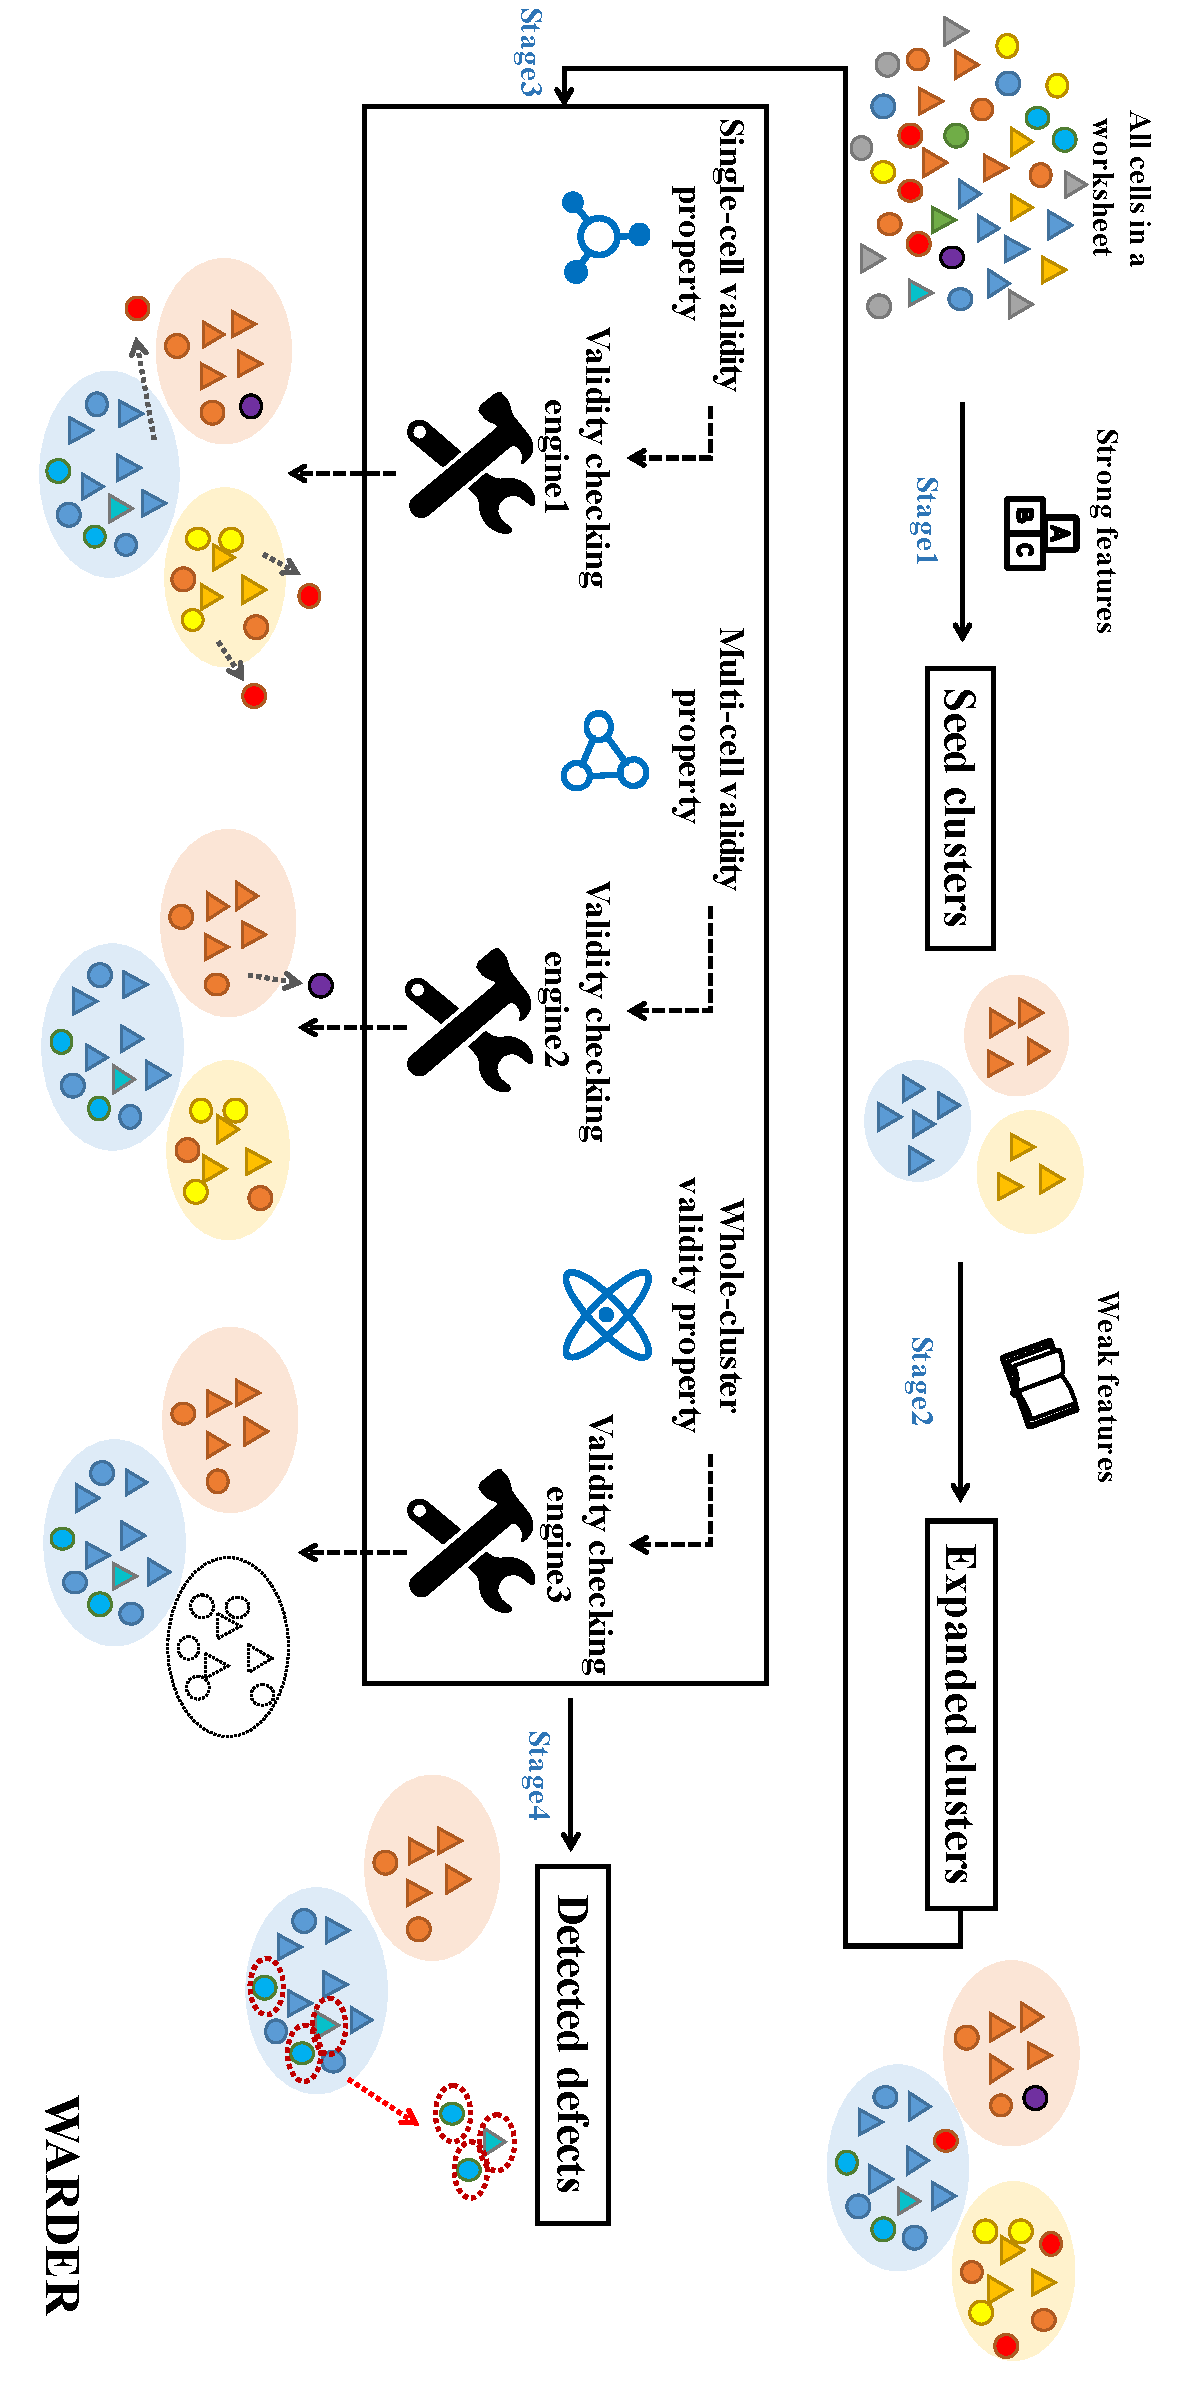
\includegraphics[width=0.7\textwidth]{figure/figure1-copy.pdf}
    \caption{\wa 的工作流程(阶段 3 是相对于它的前身 \cu 的核心贡献点)}
    \label{figure1}
\end{figure}


\section{针对单元格自身的有效性检验}
\begin{figure}[tbp]
    \centering
    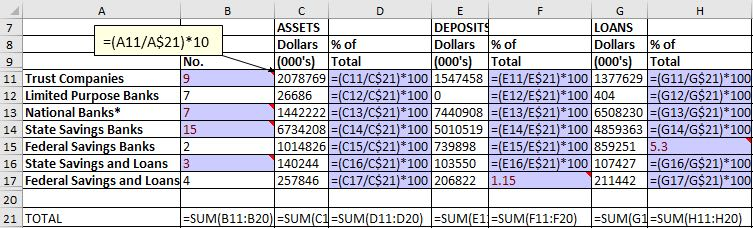
\includegraphics[width=\columnwidth]{figure/figure2.png}
    \caption{用于展现\wa 的单个单元格有效性精化方法的工作表``Summary1201''。\cu 检测出一个单元格类(用紫色标记),导致四个误报的缺陷(用红色三角标注),不过这四个单元格会被\wa 的单个单元格有效性精化方法排除出去,也就不再被错误标记为缺陷。}
    \label{figure2}
\end{figure}
第一个有效性检验方法考虑的是,当 \wa 准备将数值单元格扩充到种子类中的时候,这些被扩充的数值单元格自身是否可能拥有和种子类的计算语义相似的可能性,简称为\textit{有效性}。

在实际情况下,并没有直接的方法可以判断这些数值单元格的有效性,换言之,因为它们仅包含纯数值,无法从它自身找出和其它单元格之间的任何明显的计算语义关系。
不过,因为这些被扩充的单元格和种子类中的公式单元格即将被纳入同类,那么根据第三章中对单元格类的定义,它们应该享有一个相似的计算目标。
那么,这些被扩充的单元格的数值应当可以用某个公式单元格中含有的表达式计算出来,这是一种对数值单元格较强的约束。

为了验证这一约束,\wa 会枚举种子类中所有单元格的公式,“复制并粘贴”该公式到数值单元格中,来判断是否至少存在一个公式的计算结果和被扩充的这个单元格的值保持一致,如果保持一致,则称该数值单元格满足\textit{强有效性}。
但同时又考虑到如果数值单元格本身是含有缺陷的,那复制的公式计算的结果可能和原来的数值不同。因此,我们放宽了约束条件,当我们用一个公式来替换当前数值单元格里的内容时,只要该单元格是可计算的,即称为满足\textit{弱有效性}。
相反地,如果所有复制的公式都是不可计算的,例如复制的公式引用了错误的单元格类型,或本身包含了无效的单元格引用(比如越界),这个被扩充的数值单元格就是不满足弱有效性的,会被阻止扩充进该类中。
我们把这种方法就称为\textit{针对单元格自身的有效性检验}。
% 这里可以解释一下什么是 “用公式替换数值” 的思路

接下来,我们形式化地描述一下该检验方法。在前两个阶段得到的某以个种子类记为$SC$,对应的拓展类记为$EC$。
种子类本身是个集合,包含若干个公式单元格,记为$SC= \{c_{1}, c_{2}, \dots, c_{n}\}$,种子类中的所有公式合集记为$F_{SC}$。
同理,对应的拓展类也包含多个公式单元格,记为$EC=\{c_1, c_2, \dots, c_n, \dots, c_m\}$,其中$n \leq m$,拓展类中的所有公式合集记为$F_{EC}$。
用$eval(f|_c)$表示在单元格$c$的位置用公式$f$计算得到的数值。
当前等待检验的数值单元格记为$c_v$,它存储的数值为$v$。
上述提到的公式统一用 R1C1 表示法,原因正如第三章所述。

那么上述自然语言描述的强有效性定义如下:
\begin{definition}
    如果 $\exists f \in F_{SC},  eval(f|_{c_v}) = v$,那么就称数值单元格$c_v$满足被吸纳进$SC$中的强有效性。   
\end{definition}

对应地,弱有效性定义如下:
\begin{definition}
    如果 $\exists f \in F_{SC}, eval(f|_{c_v})$的计算过程不会触发异常,即是可计算的,那么就称数值单元格$c_v$满足被吸纳进$SC$中的弱有效性。
\end{definition}

这里我们要额外解释一下$f|_{c_v}$的含义。
该过程指用$F_{SC}$中的某个公式$f$复制粘贴到单元格$c_v$中,结合第三章对公式表达式的定义,复制粘贴过程中常量、操作符、函数名、单元格引用都保持不变。
我们在实际 \wa 实现中,使用弱有效性定义来检验单元格自身。
因为即便不能在聚类时直接确认该数值单元格具有公式缺陷,在后续的缺陷检测过程中,数值单元格仍旧会被标注为含有用常量替换的公式缺陷,并不影响最终的检测结果。

\subsection{案例分析}
如图\ref{figure2}所示,工作表“Summary1201”给出了一个案例,其中 25 个单元格(B11,B13,B14,B16,D11-17,F11-17和 H11-17)被\cu 划分为同类(用紫色标注)。
\cu 检测出了 6 个缺陷(用红色三角标注),其中 2 个(F17 和 H15)是真阳性,另外四个(B11,B13,B14 和 B16)是假阳性。
后四个数值单元格被扩充进这个类,是因为它们具有和种子类中单元格类似的弱特征(例如相似的表头和布局)。

然而,根据 \wa 的单个单元格有效性检验方法,这样的扩充是有问题的。
事实上,如果这四个单元格中的任意一个被扩充到这个类中,这个单元格把它的值和任意一个类中包含的公式计算出来的值相一致。
例如,考虑单元格 B11,按照类中包含的公式来看,对于它来说最好的潜在公式应该是“=(A11$/$A\$21)$*$100”。
然而,这个公式是不可计算的,因为单元格 A11 和 A\$21指向字符串单元格,无法参与这类除法算数运算中。
相似的问题也出现在单元格 B13、B14 和 B16。 
因此,\wa 会阻止这类数值单元格被扩充到类中。


\section{针对单元格之间关系的有效性检验}
第二个有效性检验方法考虑的是,当 \wa 用额外的数值单元格扩充种子类时,这类被扩充进来的单元格不会破坏种子类中已有单元格之间的属性。

我们拿单元格的引用举例,因为这是电子表格单元格的重要特征。
假设种子类中已有单元格的引用从不会彼此重叠,那么我们会预期一个被扩充进来的数值单元格当它被加入到这个类中,并且它的值被类中某个其他单元格的公式替换时,也不会违反这个属性。
这个预期也可以用一种相反的方式表达出来,即一个单元格类中的已有公式之间的引用已经彼此重叠了,那么对于被新扩充进来的数值单元格也不能发生不相交的情况。
也就是说,这个属性应当对类中所有的单元格保持一致(不管是原有的单元格,还是被扩充进来的单元格),这可以被看作电子表格中标的编辑风格。
另外,如果检测到违反该一致性的数值单元格,它就应当被禁止扩充到这个类中。
我们把这种方法称为\textit{针对单元格之间关系的有效性检验}。

接下来,我们形式化地描述一下该检验方法。
对引用集合交集均为空集的定义如下:
\begin{definition}
    假如$\forall c_i,c_j \in SC,\psi(f_i|_{c_i}) \cap \psi(f_j|_{c_j}) = \emptyset$,其中$f_i$为$c_i$的公式,$f_j$为$c_j$的公式,
    那么对于数值单元格$c_v$而言,如果$\exists f_k \in F_{SC}, \forall c_i \in SC, \psi(f_k|_{c_v}) \cap \psi(f_i|_{c_i}) = \emptyset$,
    则称单元格$c_v$满足针对单元格之间关系的空集有效性。
\end{definition}

相应地,对引用集合交集均为非空的定义如下:
\begin{definition}
    假如$\forall c_i,c_j \in SC,\psi(f_i|_{c_i}) \cap \psi(f_j|_{c_j}) \neq \emptyset$,其中$f_i$为$c_i$的公式,$f_j$为$c_j$的公式,
    那么对于数值单元格$c_v$而言,如果$\exists f_k \in F_{SC}, \forall c_i \in SC, \psi(f_k|_{c_v}) \cap \psi(f_i|_{c_i}) \neq \emptyset$,
    则称单元格$c_v$满足针对单元格之间关系的非空集有效性。 
\end{definition}

在第三章我们定义过针对公式表达式的引用集合$\sigma(exp)$,这里的$\psi(f|_c)$类似,表示将 R1C1 表示法下的公式$f$套用在单元格$c$上,单元格$c$实际引用的具体单元格集合。比如单元格C3套用上公式RC[-2]+RC[-1],则对应的$\sigma$(RC[-2]+RC[-1])为\{RC[-2],RC[-1]\},而$\psi$((RC[-2]+RC[-1])$|_{C3}$)为\{A3,B3\}。

\subsection{案例分析}
\begin{figure}[tbp]
    \centering
    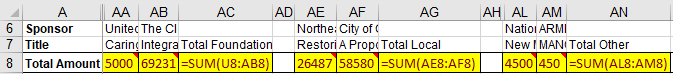
\includegraphics[width=\columnwidth]{figure/figure3.png}
    \caption{用于展现\wa 的多个单元格有效性精化方法的工作表``Detail for the College of A\&S''。\cu 检测出一个单元格类(用黄色标记),并进而导致六个假阳性的缺陷被报告出来(用红色三角形标注),不过这六个单元格会被\wa 的多单元格有效性精化方法从类中排除出去,进而不会再被错误的标记为有缺陷的单元格。}
    \label{figure3}
\end{figure}
如图\ref{figure3}所示,工作表“Detail for the College of A\&S” 给出了一个案例。
其中,9 个单元格(AA8, AB8, AC8, AE8, AF8, AG8, AL8, AM8和AN8)被\cu 划分到同一个类中(用黄色标记)。
接着,\cu 检测出 6 个单元格缺陷(AA8, AB8, AE8,AF8,AL8和AM8),因为它们只包含纯数值,但这六个缺陷都是假阳性。

不过,\wa 能够阻止这六个单元格(AA8, AB8, AE8,AF8,AL8和AM8)被扩充进来,从而避免了这 6 个误报的情况。
事实上,这 6 个数值单元格并不和其它 3 个公式单元格(AC8,AG8和AN8)共享相同的计算语义。
前面的数值单元格代表了用户直接给出的具体的数值,而另外三个公式则是计算它们各自左侧的若干个单元格的和。

\wa 通过它的多个单元格有效性检验方法区分出这两类:后三个公式单元格的引用范围是互不重叠的,但如果把前面 6 个数值单元格扩充进来,并用任意一个公式来替换它们的值,这个属性会遭到破坏。
例如,当把单元格 AF8 中的数值用单元格 AG8 里的公式模板替换成公式“=SUM(AD8:AE8)”时,它的引用单元格(AD8 和 AE8)会和单元格 AG8 的引用单元格(AE8 和 AF8)发生重叠。
相似的问题也会出现在单元格 AA8,AB8,AE8,AL8 和 AM8 上。
因此,\wa 会禁止这类数值单元格被扩充到类中。


\section{针对整个类的有效性检验}
第三种有效性检验方法考虑的是最终形成单元格类的整体有效性,即它关注于类层面而不是单元格层面的有效性属性。

我们预期在每个单元格类中应该存在一个统一的公式能够覆盖大多数单元格,也就是说大多数单元格应当遵循一个共同的计算语义。
\wa 会测试类中所有现存可获得的公式,如果没有任何一个能够满足这个目的,\wa 就会认定这个类不是有效的,并将该类从所有类的集合中删除,以避免后续在缺陷检测过程中将其中的过半数量的单元格标记为含有公式缺陷,即产生大量缺陷误报。
我们把这种方法称为\textit{针对整个类的有效性检验}。

接下来,我们形式化地描述一下该检验方法。
我们首先定义一个辅助函数:
\begin{definition}
    对于一个公式$f_i \in F_{EC}$和某个公式单元格$c$及其自身包含的公式$f$来说,定义辅助函数$\rho$为
    $
    \rho(f_i, c) = 
    \left\{
        \begin{aligned}
        & 1     & eval(f_i|_c) == eval(f|_c); \\
        & 0     & otherwise. \\
        \end{aligned}
    \right.
    $
    如果$\rho(f_i,c)$为 1,则我们称公式$f_i$可以用来覆盖单元格$c$且计算出的新值与原有公式计算的值相等。
\end{definition}

接着我们定义:
\begin{definition}
    如果$\exists f_i \in F_{EC}, (\sum_{j = 1}^{m} \rho(f_i, c_j)) > \theta  * size(F_{EC})$,
    则我们称该扩展单元格类存在一个能覆盖超过$\theta  * size(F_{EC})$数量的公式单元格的统一公式,即该单元格类满足针对整个类的强有效性。
\end{definition}

如果我们把辅助函数等于 $1$ 的条件适当放宽,即要求$\frac{|eval(f_i|_c)-eval(f|_c)|}{eval(f|_c)} \leq \epsilon$,即新值与旧值的差的绝对值占旧值的比例小于给定的阈值$\epsilon$,
则相应地,我们就得到了关于该单元格类满足针对整个类的弱有效性定义。在实验评估中,$\epsilon$取值为0.01,即我们容忍较小程度的计算结果偏差,如果偏差较大,说明该单元格很可能不应该被此公式覆盖。
我们这里只是枚举公式集合$F_{EC}$中的公式来尝试覆盖整个单元格类,而没有使用类似基于组件的程序合成方法来为整个类合成一个最为适宜的公式。
这样的做法有两点考虑:第一,使用程序合成算法通常会大大降低执行效率,让终端用户的等待时间更久;
第二,每个单元格类中的公式通常比较简单,相似度高,在公示集合中存在备选公式的概率较高,没有必要动用相对复杂的程序合成工具。

在\wa 的实际系统实现中,我们采用针对整个类的弱有效性定义来过滤不合格的单元格类,因为我们要容忍某些公式单元格是有缺陷的,因而计算出来的值有一定偏差可以允许。
在后续的缺陷检测环节,我们有很大把握将其检测出来。

\subsection{案例分析}
\begin{figure}[tp]
    \centering
    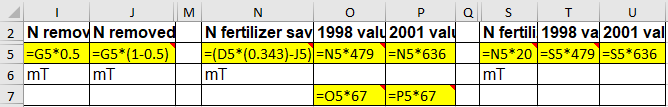
\includegraphics[width=\columnwidth]{figure/figure4.png}
    \caption{用于展现\wa 的整个类有效性检验方法的工作表``World 1996''。\cu 识别出了一个类(用花色标记出来,但整个类是不合理的),进而导致所有相关的单元格都被错误地标记为有缺陷的(用红色三角形标记),不过这个类会被\wa 的整个类的有效性检验方法移除掉,进而相关的所有单元格也不会被错误地标记为有缺陷的。}
    \label{figure4}
\end{figure}
如图\ref{figure4}所示,工作表“World 1996”给出了一个案例。
其中,\cu 把 10 个单元格划分为同一个类(用黄色标注)。
进而 \cu 把其中的 7 个检测为有缺陷的单元格,但这 7 个都是假阳性。

事实上,这10 个单元格包含几乎完全不同的公式(5 种计算模式),这强烈地表明它们本质上遵循不同的计算语义。
通过我们的类级别的有效性检验方法,\wa 会将该类完整地从类集合中删除。
这里需要注意的是,\wa 需要一个阈值来控制“覆盖大多数单元格”这个判断的程度,即确定阈值$\theta$。
安全起见,\wa 选择一个保守的值,即 50\%,来尽可能保护单元格类不被排除在外(作为对比,\ca 选择了相对激进的值70\%)。


\section{有效性检验方法的综合应用}
其实前面三节我们给出了设计有效性检验方法的逻辑框架,本文仅是在三个层面上分别设计了最为基础但也最为实用的有效性检验方法,在第六章的实验评估中也取得了较好的效果,说明进行有效性检验方法本身的思路是成立的,的确解决了\cu 存在的技术缺陷,未来工作可以在三个层面上进行更细致的有效性检验方法设计和改良。

根据上述设计的三个有效性检验方法之间的层次关系,\wa 将三个方法依次应用在 \cu 的第二阶段单元格聚类之后,即依次使用针对单元格自身、针对单元格之间关系和针对整个类的有效性检验方法。
它们三者彼此互补,构成了针对单元格聚类的有效性检验方法的有机整体。
它们的目标是提升单元格聚类有效性,使得聚类结果更加具有稳定和可靠。

稳定可靠的单元格聚类结果,最终也会对缺陷检测起到积极作用,如极大地减少公式缺陷的误报数量和误报率,这部分也会在第六章的实验评估部分进行验证。
\chapter{工具实现与演示}

本章

\section{Excel 插件测试工具 EGuard}
\eg 插件测试工具使用 JavaScript 语言实现,可在 Excel 软件中直接加载并使用的第三方插件,采用 Microsoft Office-js \footnote{https://github.com/OfficeDev/office-js} 框架来异步读写和操作 Excel 文件。
只要是 Excel 可以运行的平台,如 Windows,MacOS 或者在浏览器中打开的 Excel OneDrive 应用上,都可以加载我们的\eg 插件。
相应的工具源码发布在 GitHub 上\footnote{https://github.com/dlee992/EGuard}。

目前,\eg 测试工具的实现包含约 3100 行 JavaScript、HTML 和 CSS 代码,其中包含约 2400 行核心功能代码和约 700 行图形界面代码,后续还会继续更新到一个更加完善的版本,然后发布到 Excel 第三方插件平台上,供任意用户下载使用。

\subsection{EGuard 插件架构}
\begin{figure}[tp]   
    \centering
    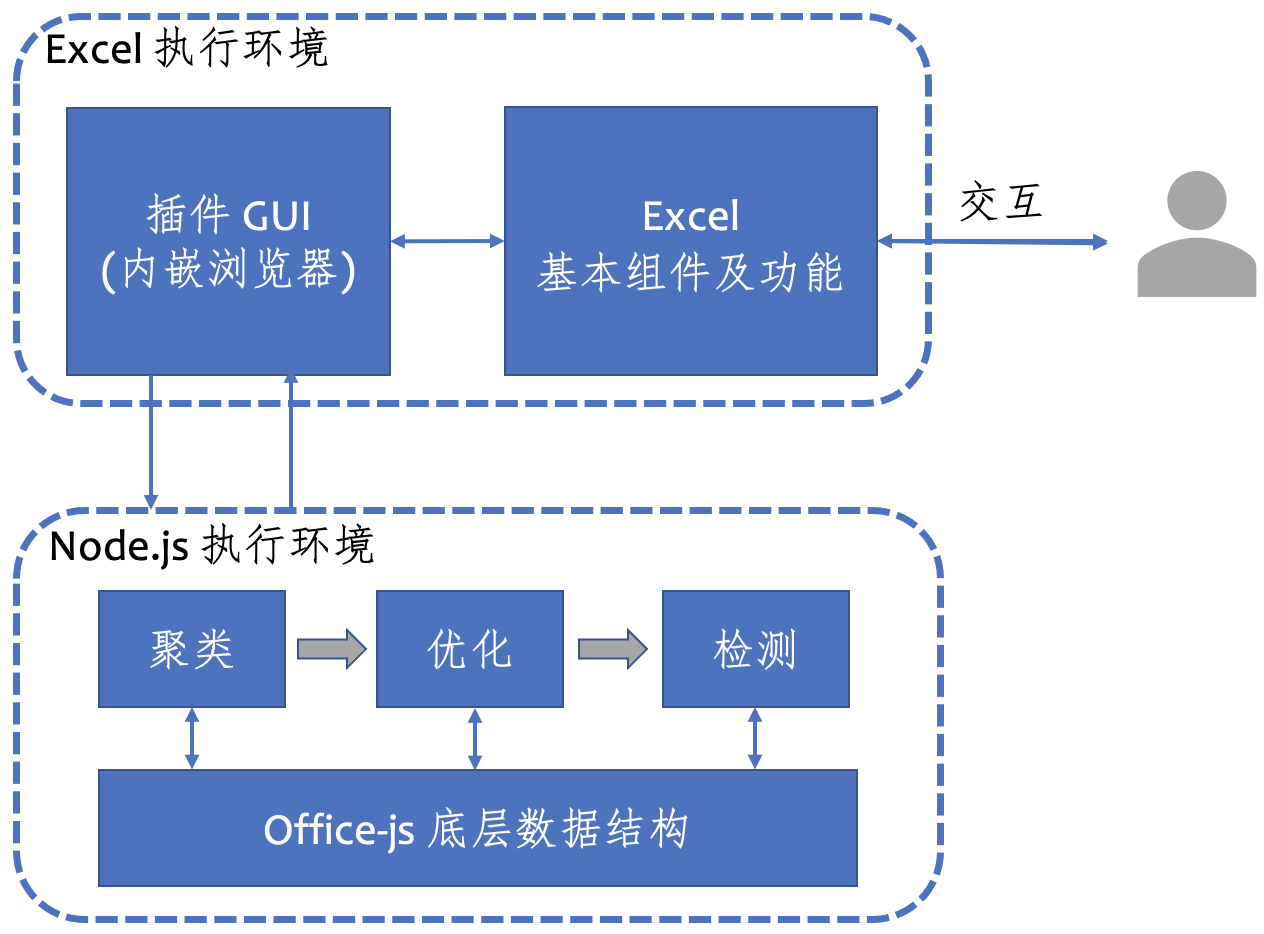
\includegraphics[width=0.8\textwidth]{figure/eg/eguard-framework.png}
    \caption{\eg 软件架构示意图}
    \label{figure-eg-framework}
\end{figure}


\begin{figure}[tp]   
    \centering
    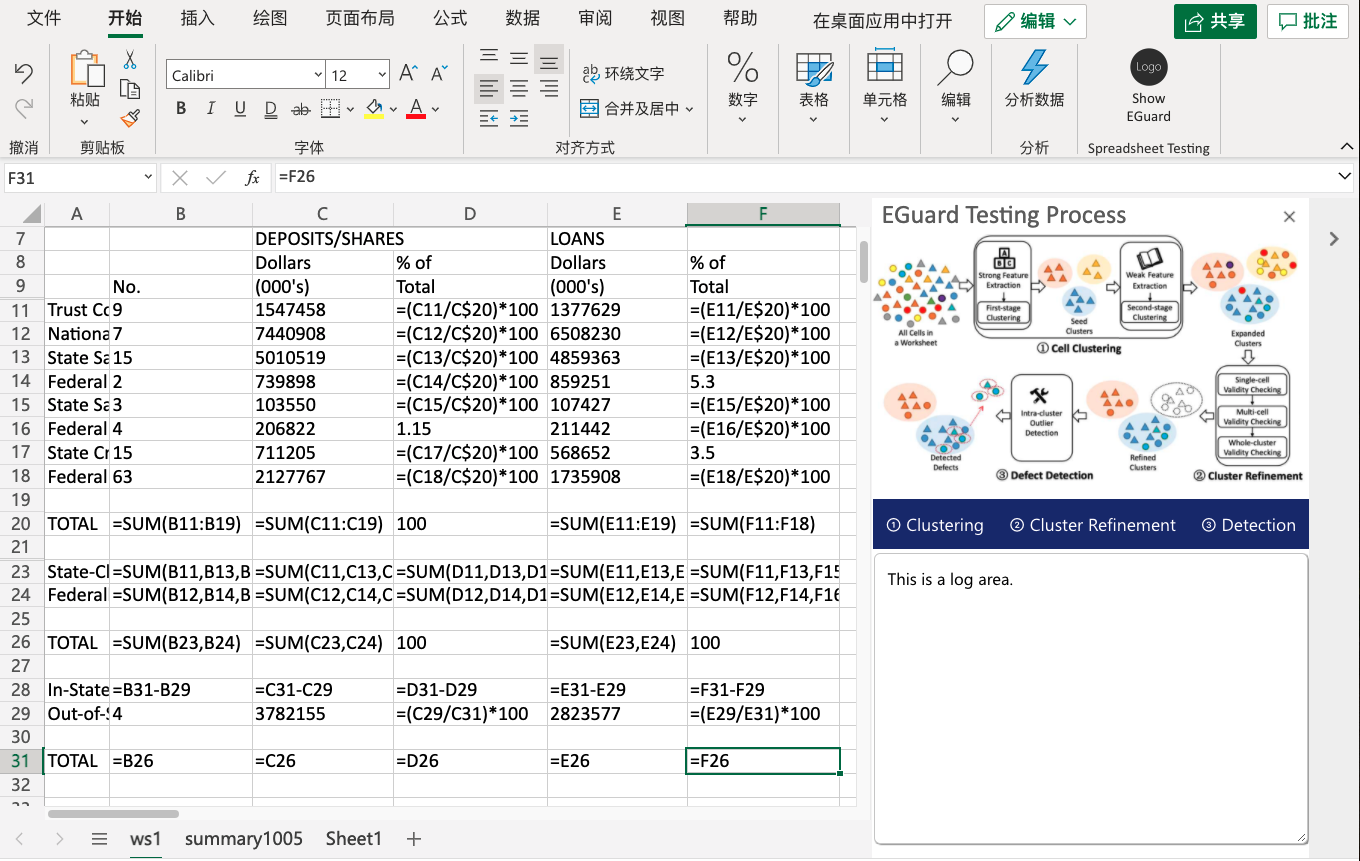
\includegraphics[width=\textwidth]{figure/eg/eguard-1.png}
    \caption{\eg 的插件布局}
    \label{figure-eg1}
\end{figure}
\begin{figure}[tbp]    
    \centering
    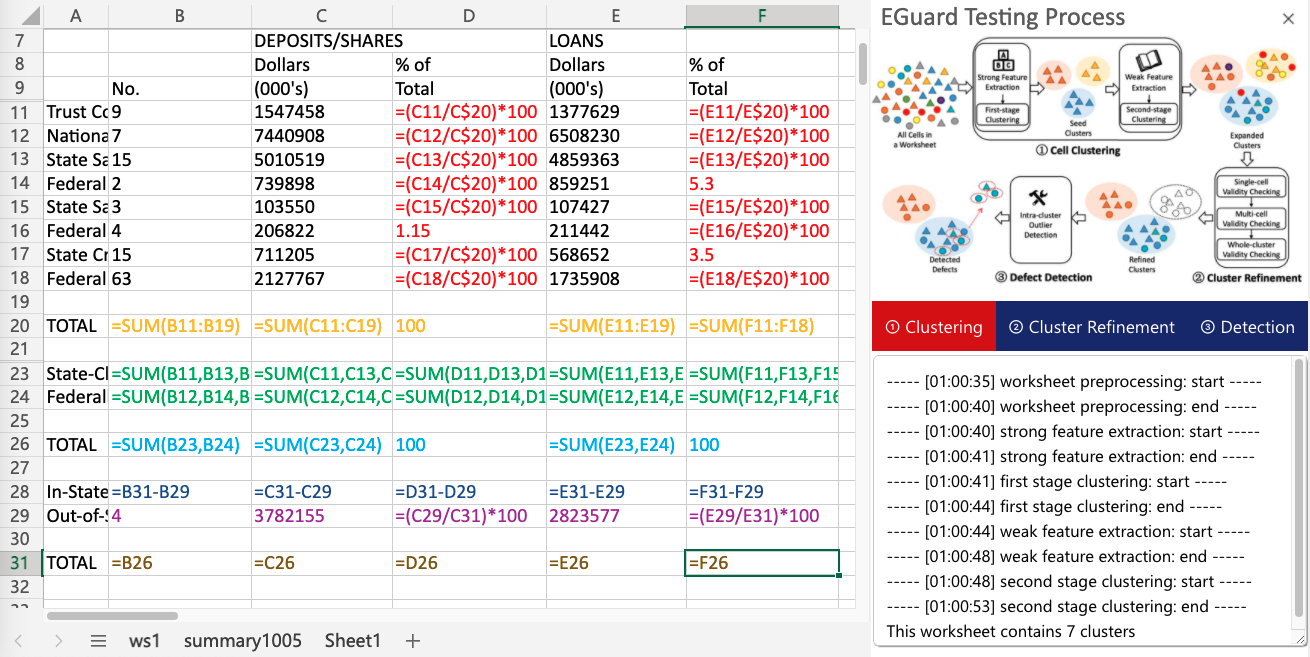
\includegraphics[width=\textwidth]{figure/eg/eguard-2.png}
    \caption{\eg 执行单元格聚类后的电子表格标记和执行信息输出}
    \label{figure-eg2}
\end{figure}
\begin{figure}[tbp]    
    \centering
    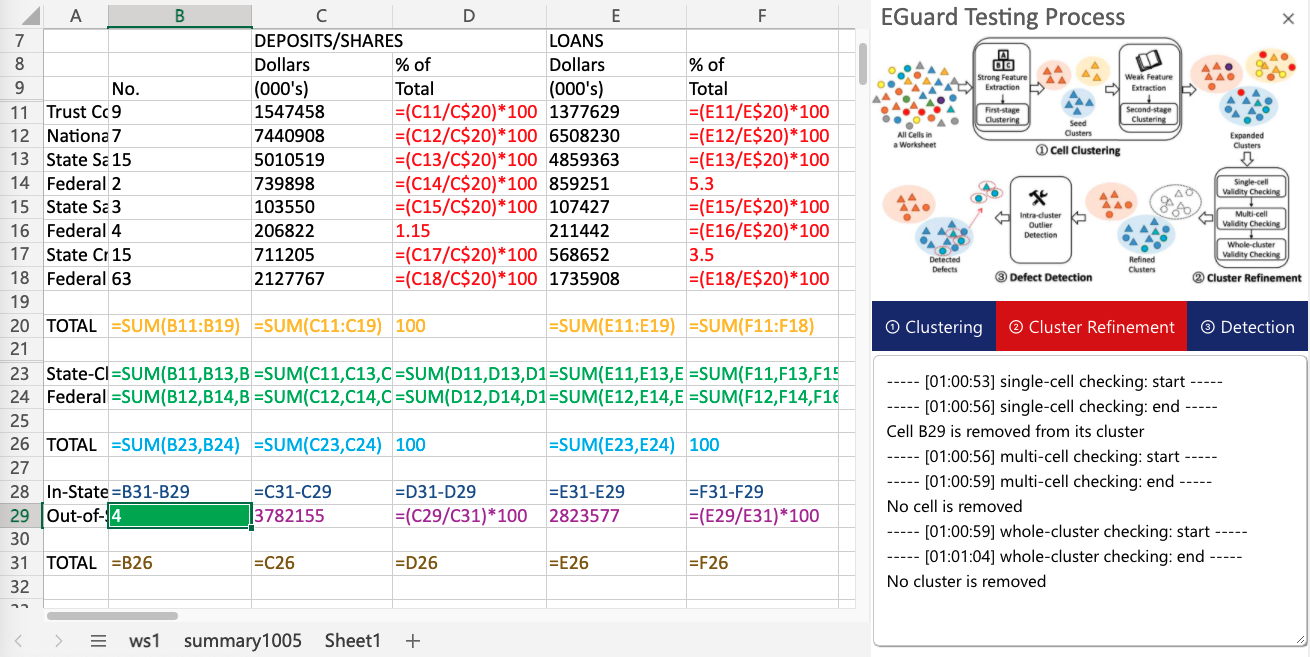
\includegraphics[width=\textwidth]{figure/eg/eguard-3.png}
    \caption{\eg 执行三个单元格检验方法后的电子表格标记和执行信息输出}
    \label{figure-eg3}
\end{figure}
\begin{figure}[tp]   
    \centering
    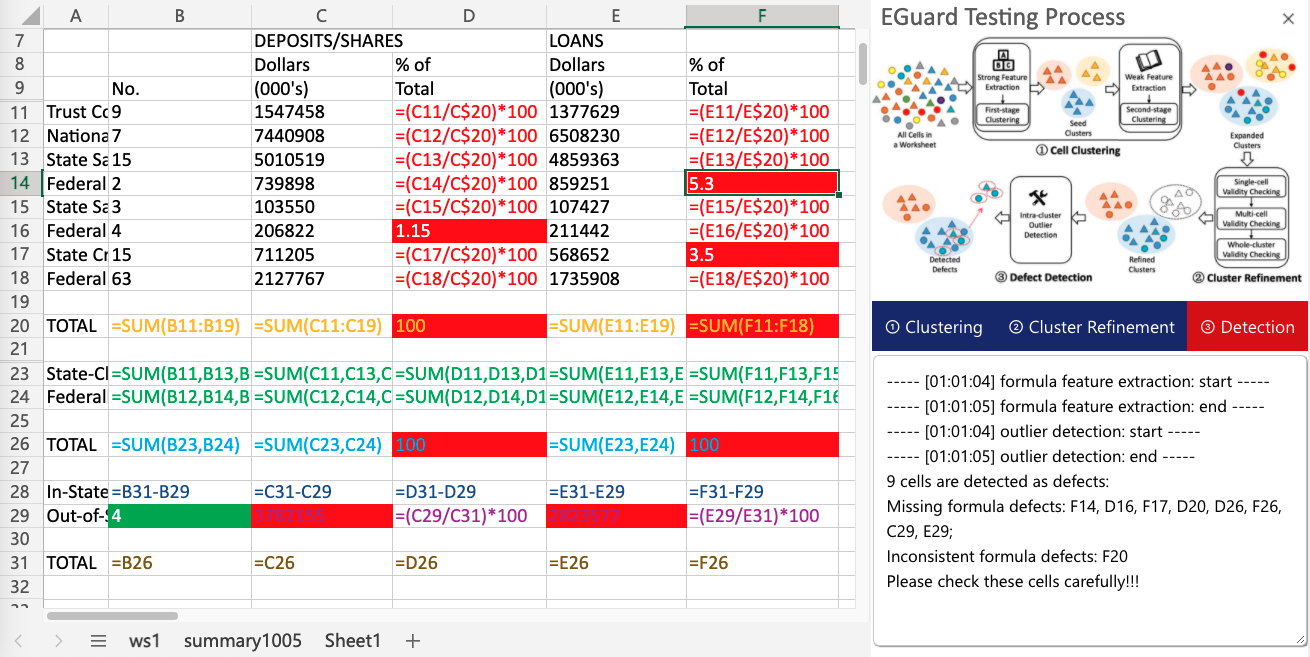
\includegraphics[width=\textwidth]{figure/eg/eguard-4.png}
    \caption{\eg 执行缺陷检测后的电子表格标记和执行信息输出}
    \label{figure-eg4}
\end{figure}

\subsection{界面设计}
如图\ref{figure-eg1}所示,在 Excel 软件中,从“插入”菜单栏选择“Office 加载项”按钮,然后选择本地的插件 \eg 进行加载。
加载完毕后,在“开始”菜单栏的最右侧会显示我们的插件工具图标,点击图标即显示出图\ref{figure-eg1}右侧的内嵌式网页,其标题是“EGuard Testing Process”。
整个内嵌式网页包含如下三个部分:

\begin{enumerate}
    \item 上方显示\eg 插件工具的执行流程图,方便终端用户对检测过程有一个直观感性的认识;
    \item 中间部分为一组选项卡,含有三个执行选项,依次为“\ding{172} Clustering”(两阶段的单元格聚类)、“\ding{173} Cluster Refinement”(基于有效性属性的检验) 和 “\ding{174} Detection”(缺陷检测);
    \item 下方是执行信息输出区域,显示执行的流程和对应的时间戳,以及一些帮助终端用户更好地理解检测结果的辅助信息。
\end{enumerate}

\subsection{使用展示}
接下来,我们结合一个具体的工作表来展示 \eg 的完整使用流程:
\begin{enumerate}
    \item 如图\ref{figure-eg1}所示,首先我们打开一个想要进行测试的 Excel 文件,并切换到想要进行测试的工作表,图中我们打开电子表格“illustrative\_example.xlsx”的工作表“ws1”,按上述方式加载 \eg 插件并在右侧打开嵌入式网页,为了方便观察聚类结果,我们把 Excel 的公式显示选项打开(默认显示 A1 表示法的公式形式);
    
    \item 如图\ref{figure-eg2}所示,点击“\ding{172} Clustering”选项卡按钮,即开始对当前工作表执行强弱特征抽取和两阶段的单元格聚类任务,在插件下方可以看到具体的执行流程包括每个子任务对应的执行时长和一些辅助用户理解的信息。如图所示,最终通过两阶段聚类检测到了 7 个单元格类,并在工作表中用不同的字体颜色标注出来;
    
    \item 如图\ref{figure-eg3}所示,点击“\ding{173} Cluster Refinement”选项卡按钮,即在两阶段聚类的基础上执行针对本文提出的\wa 方法,即第四章描述的 3 种基于有效性属性的检验方法。在当前示例中,依据单个单元格有效性属性检验结果,将单元格 B29 从原先的单元格类 \{B29,C29,D29,E29,F29\} 中移除,因为该单元格并不具备和其他单元格类似的除法运算语义,即如果 B29 具有类似公式,则会显示为=(A29$/$A31)$*$100,但 A29 和 A31 都是字符串单元格,无法进行数值运算。从表中可观察到,被移除的单元格会用绿色背景和白色字体标注出来;
    
    \item 如图\ref{figure-eg4}所示,点击“\ding{174} Detection”选项卡按钮,即在聚类和检验的基础上,进行类内缺陷检测,在当前工作表中,分别从 4 个单元格类中检测出 9 个有缺陷的单元格,其中 8 个为含有常量替换的公式缺陷的单元格,即 F14、D16、F17、D20、D26、F26、C29 和 E29,以及 1 个引用替换的公式缺陷的单元格 F20。从工作表中可观察到,有缺陷的单元格会用红色背景标注出来,如果原来该单元格就是红色字体,为显示结果清晰,则相应改为白色字体,如单元格 D16;
    
    \item 最后,用户可以结合工作表中的标注信息(字体颜色和背景色)和插件下方的日志信息,对工具标记为有公式缺陷的单元格进行检查和修订。
\end{enumerate}



\section{集成化测试工具 \sg }
\sg 工具也是使用 Java 实现的可视化集成工具,同样使用 Apache POI 库来读写 Excel 格式的电子表格。
和\wa 类似,目前只能在 Windows 操作系统下执行。
\sg 的初始核心代码是由张瑞青师兄开发,我们额外添加了两个新技术模块,\cu-OPT\footnote{原\cu 技术的 bug 修复版本} 和 \wa ,并进行了对应的集成编码工作。
相应的工具介绍主页发布在 GitHub Pages 上 \footnote{https://sheetguard.github.io/sguard/},其中包含了工具源码链接和介绍性的视频链接,发布在 YouTube \footnote{https://www.youtube.com/watch?v=gNPmMvQVf5Q} 和 Bilibili \footnote{https://www.bilibili.com/video/BV1x4411g7do} 网站上。

\sg 工具的完整实现包含约 10,500 行 Java 代码,其中包含约 7,300 行核心代码和约 3,200 行图形界面代码。

\subsection{SGuard 工具架构}
\begin{figure}[tp]   
    \centering
    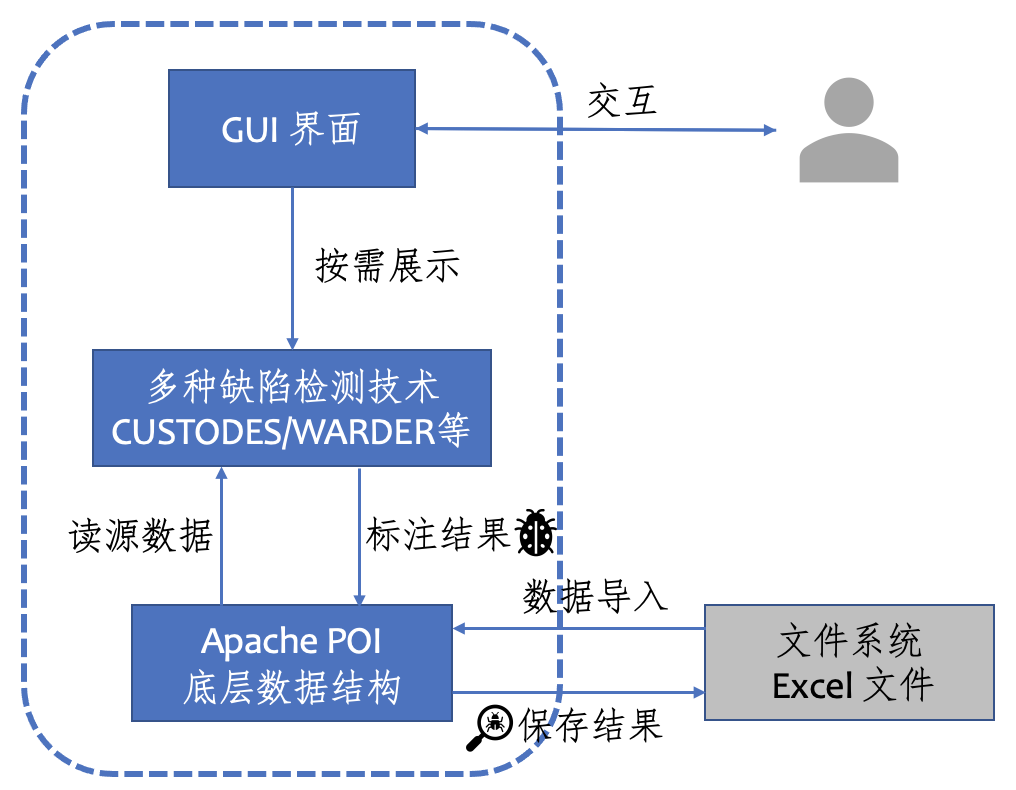
\includegraphics[width=0.8\textwidth]{figure/sg/sguard-framework.png}
    \caption{\sg 架构展示}
    \label{figure-sg-framework}
\end{figure}

\subsection{界面设计}
\begin{figure}[tbp]    
    \centering
    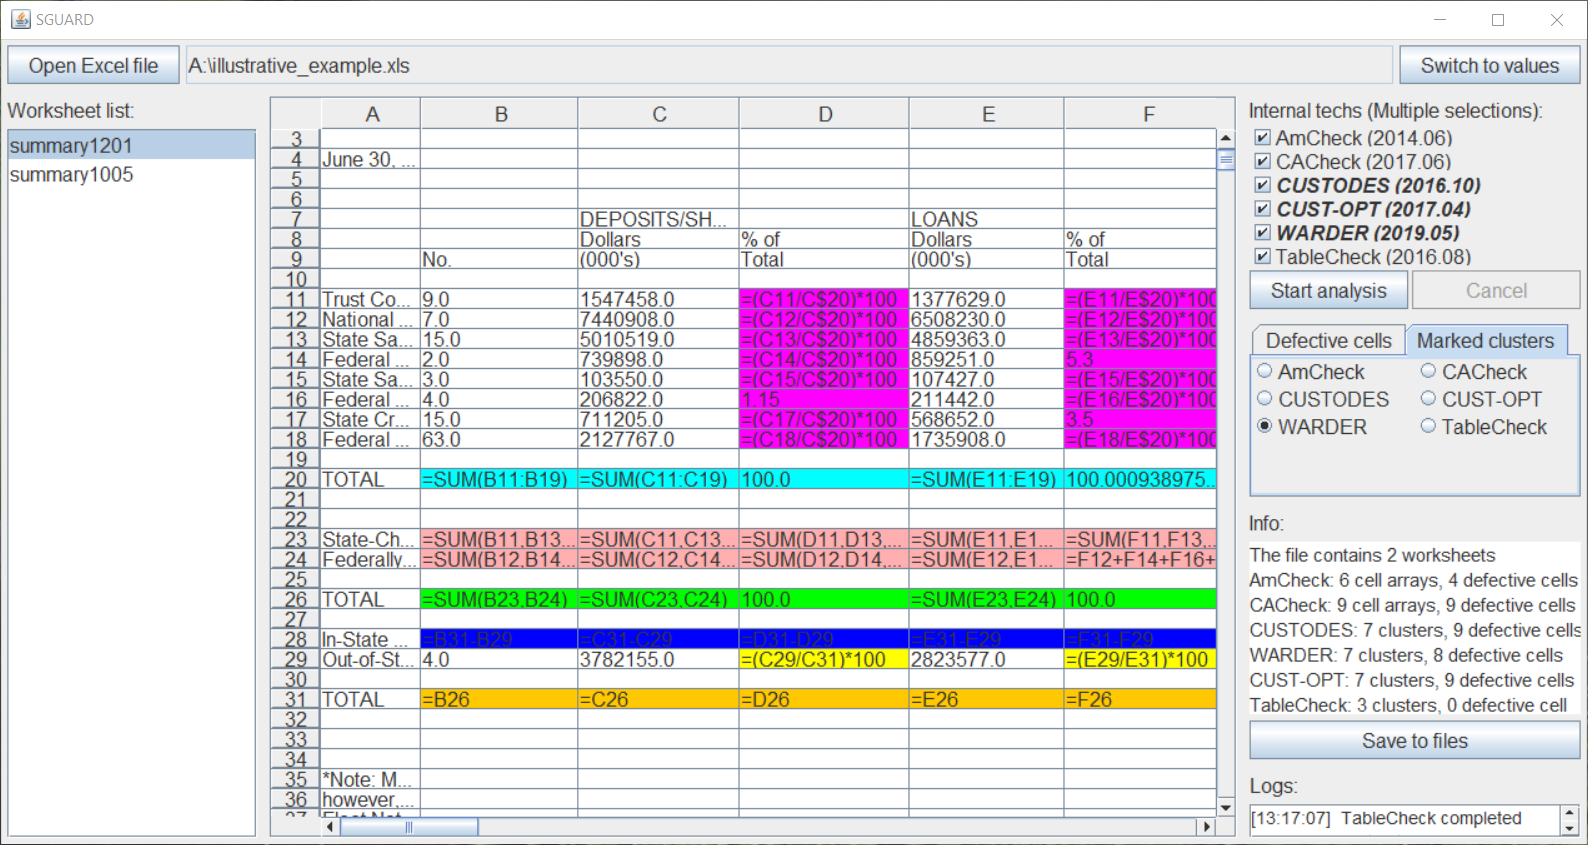
\includegraphics[width=\textwidth]{figure/figure11.png}
    \caption{\sg 的使用截图}
    \label{figure11}
\end{figure}
% \begin{figure}[tbp]    
    \centering
    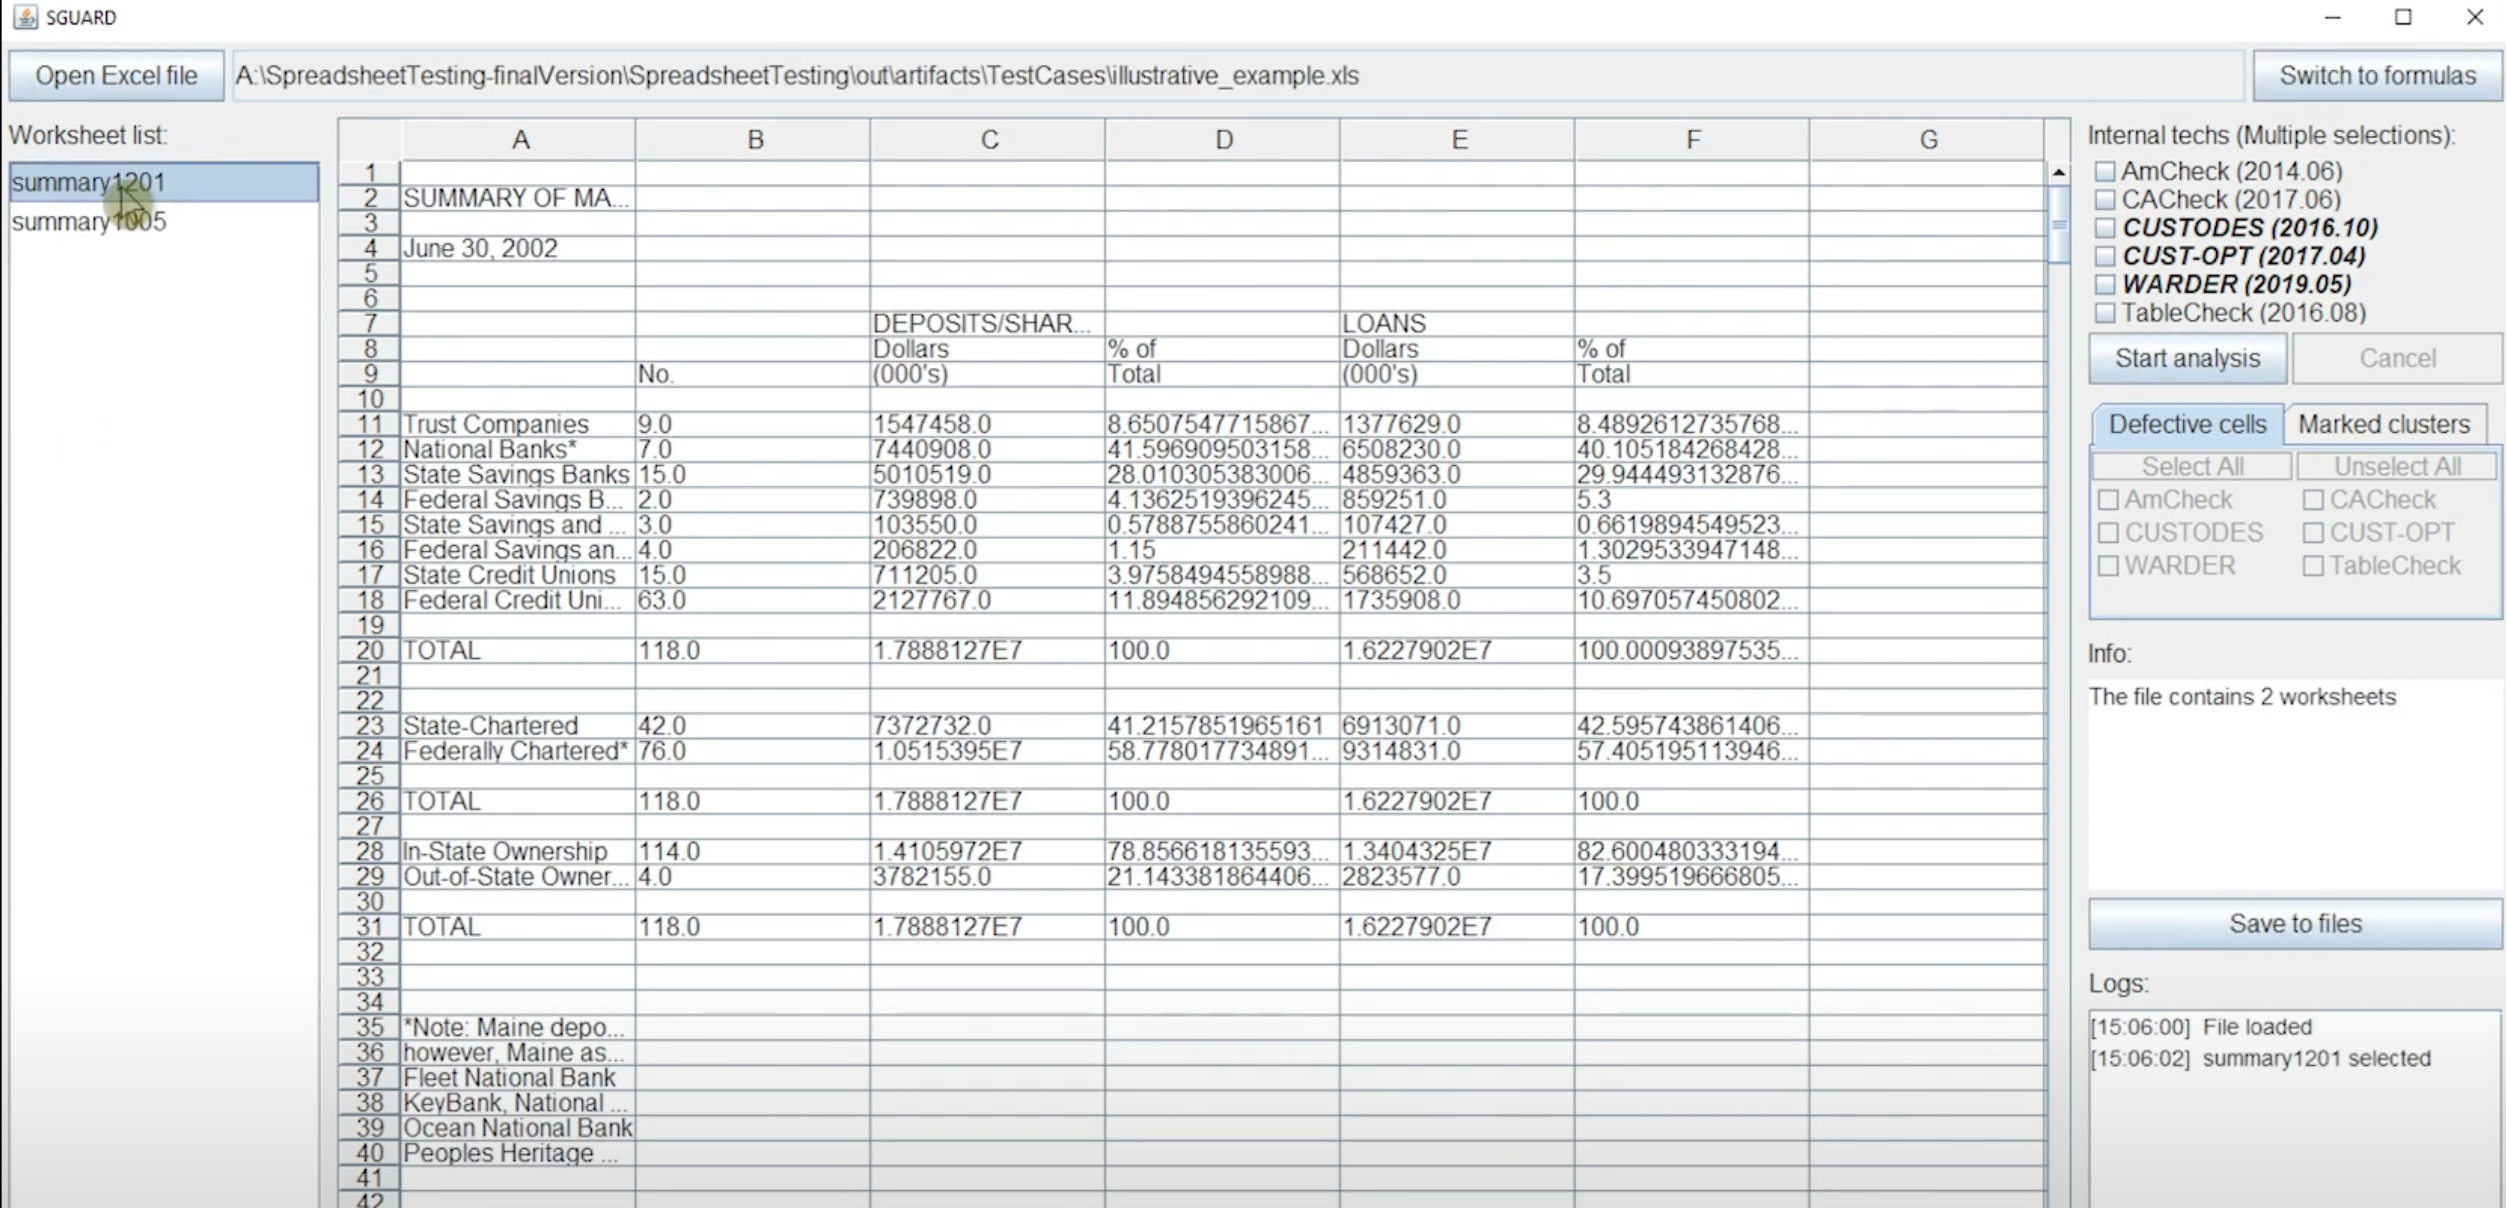
\includegraphics[width=\textwidth]{figure/sg/sguard-3.png}
    \caption{\sg 的使用流程演示截图 3}
    \label{figure-sg3}
\end{figure}
\begin{figure}[tbp]    
    \centering
    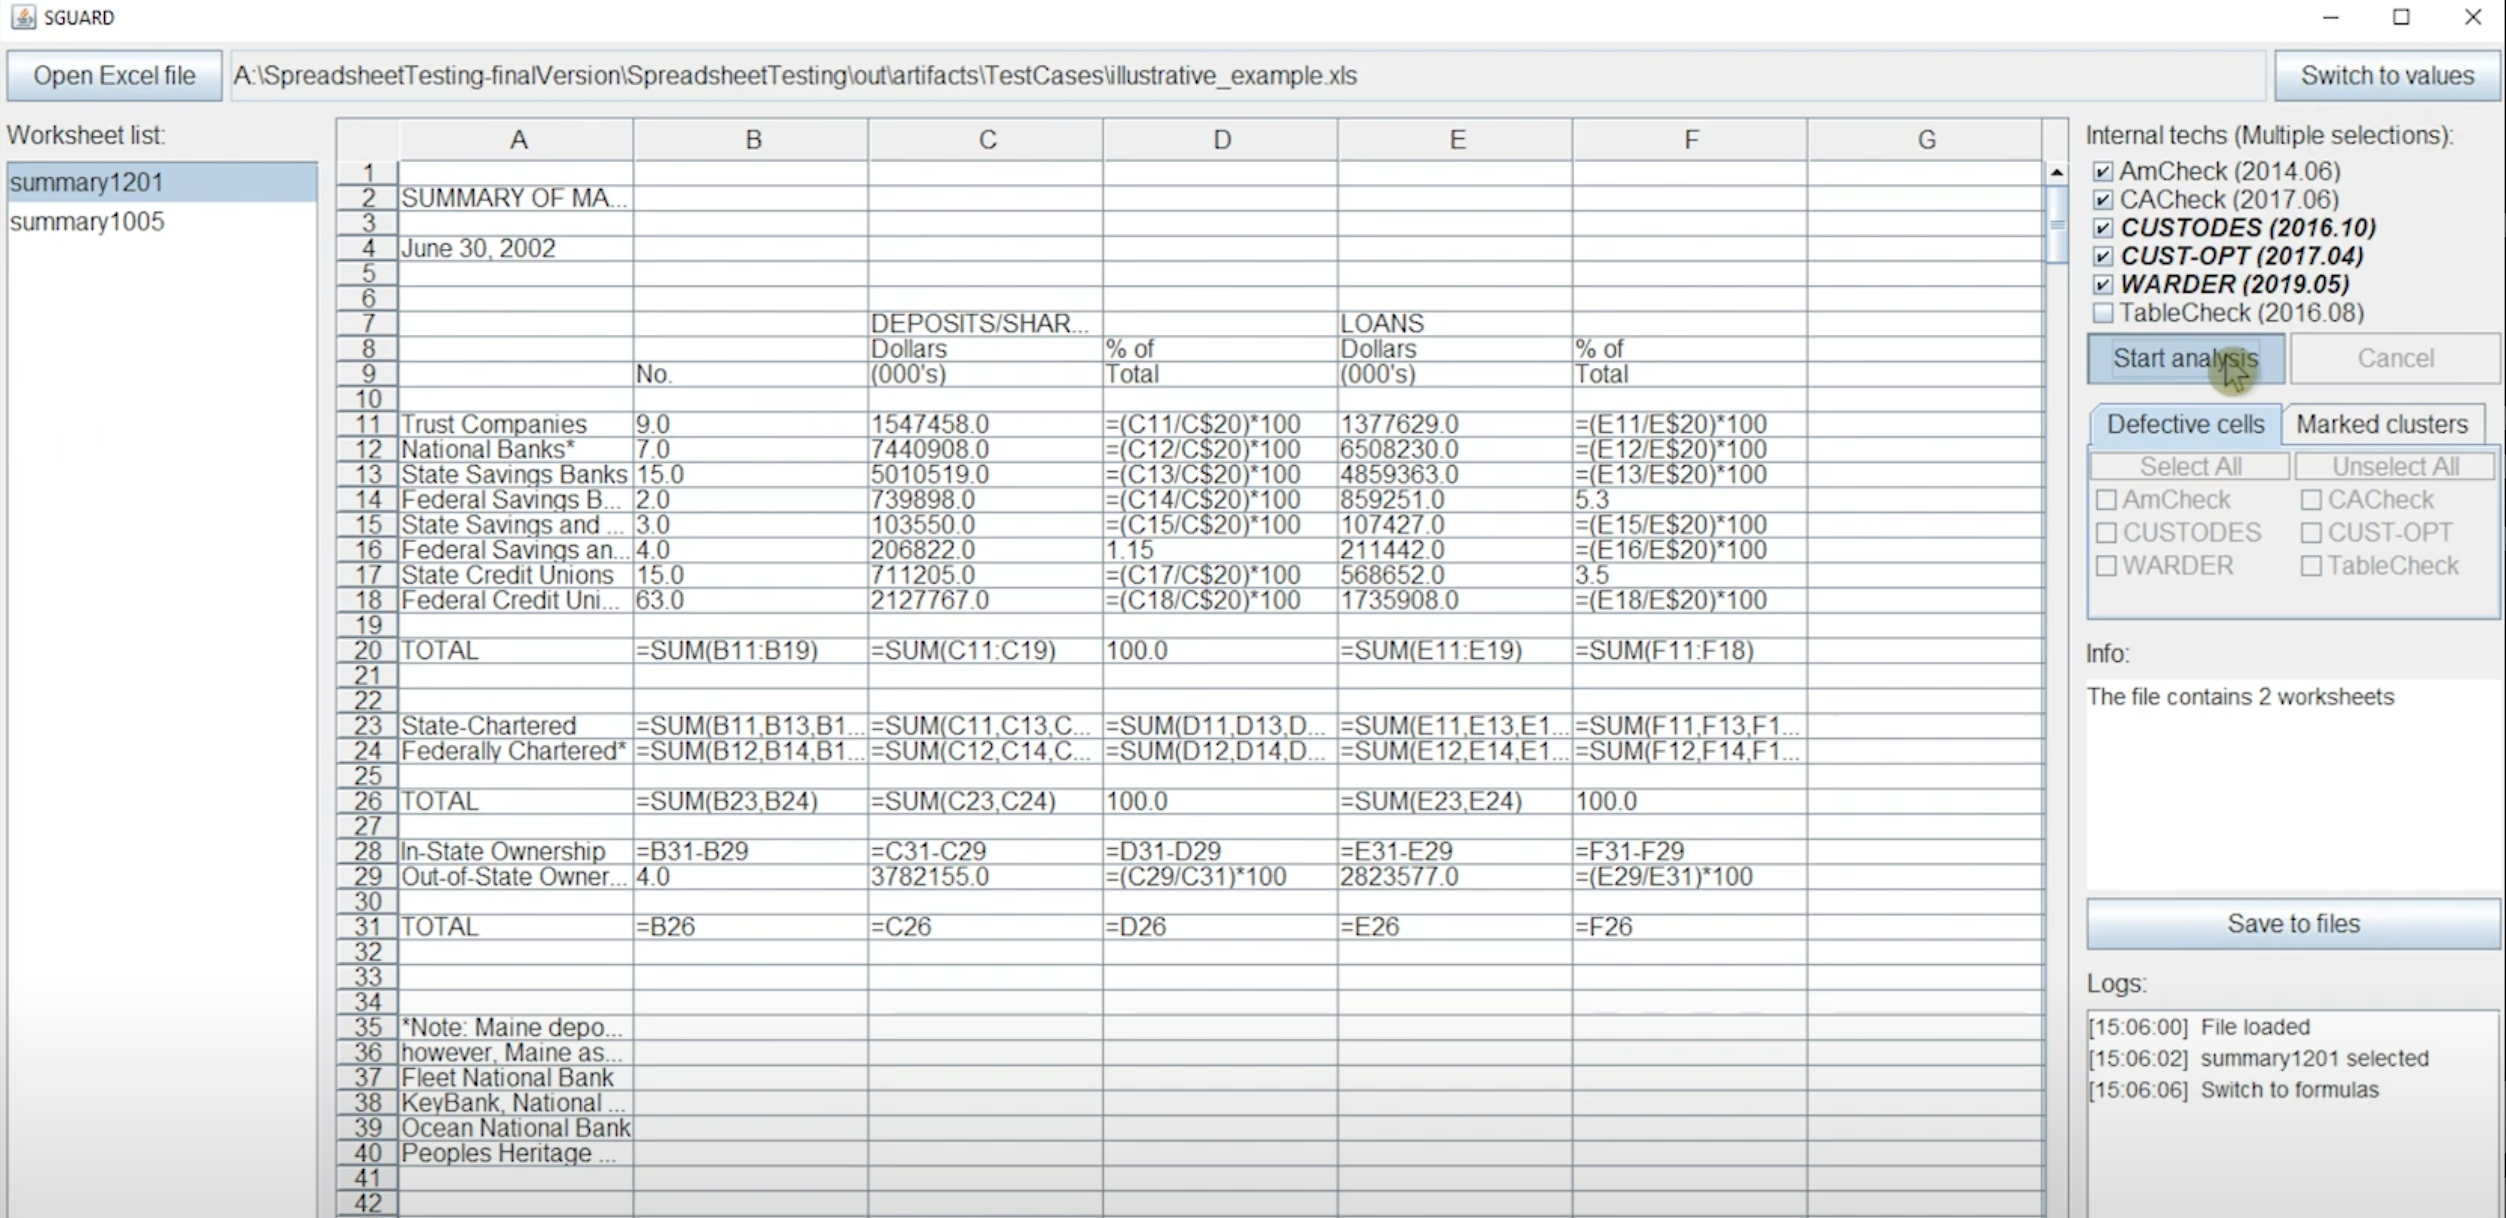
\includegraphics[width=\textwidth]{figure/sg/sguard-4.png}
    \caption{打开待测电子表格并选择待测工作表,再选择要执行的缺陷检测技术并开始执行}
    \label{figure-sg4}
\end{figure}
\begin{figure}[tbp]    
    \centering
    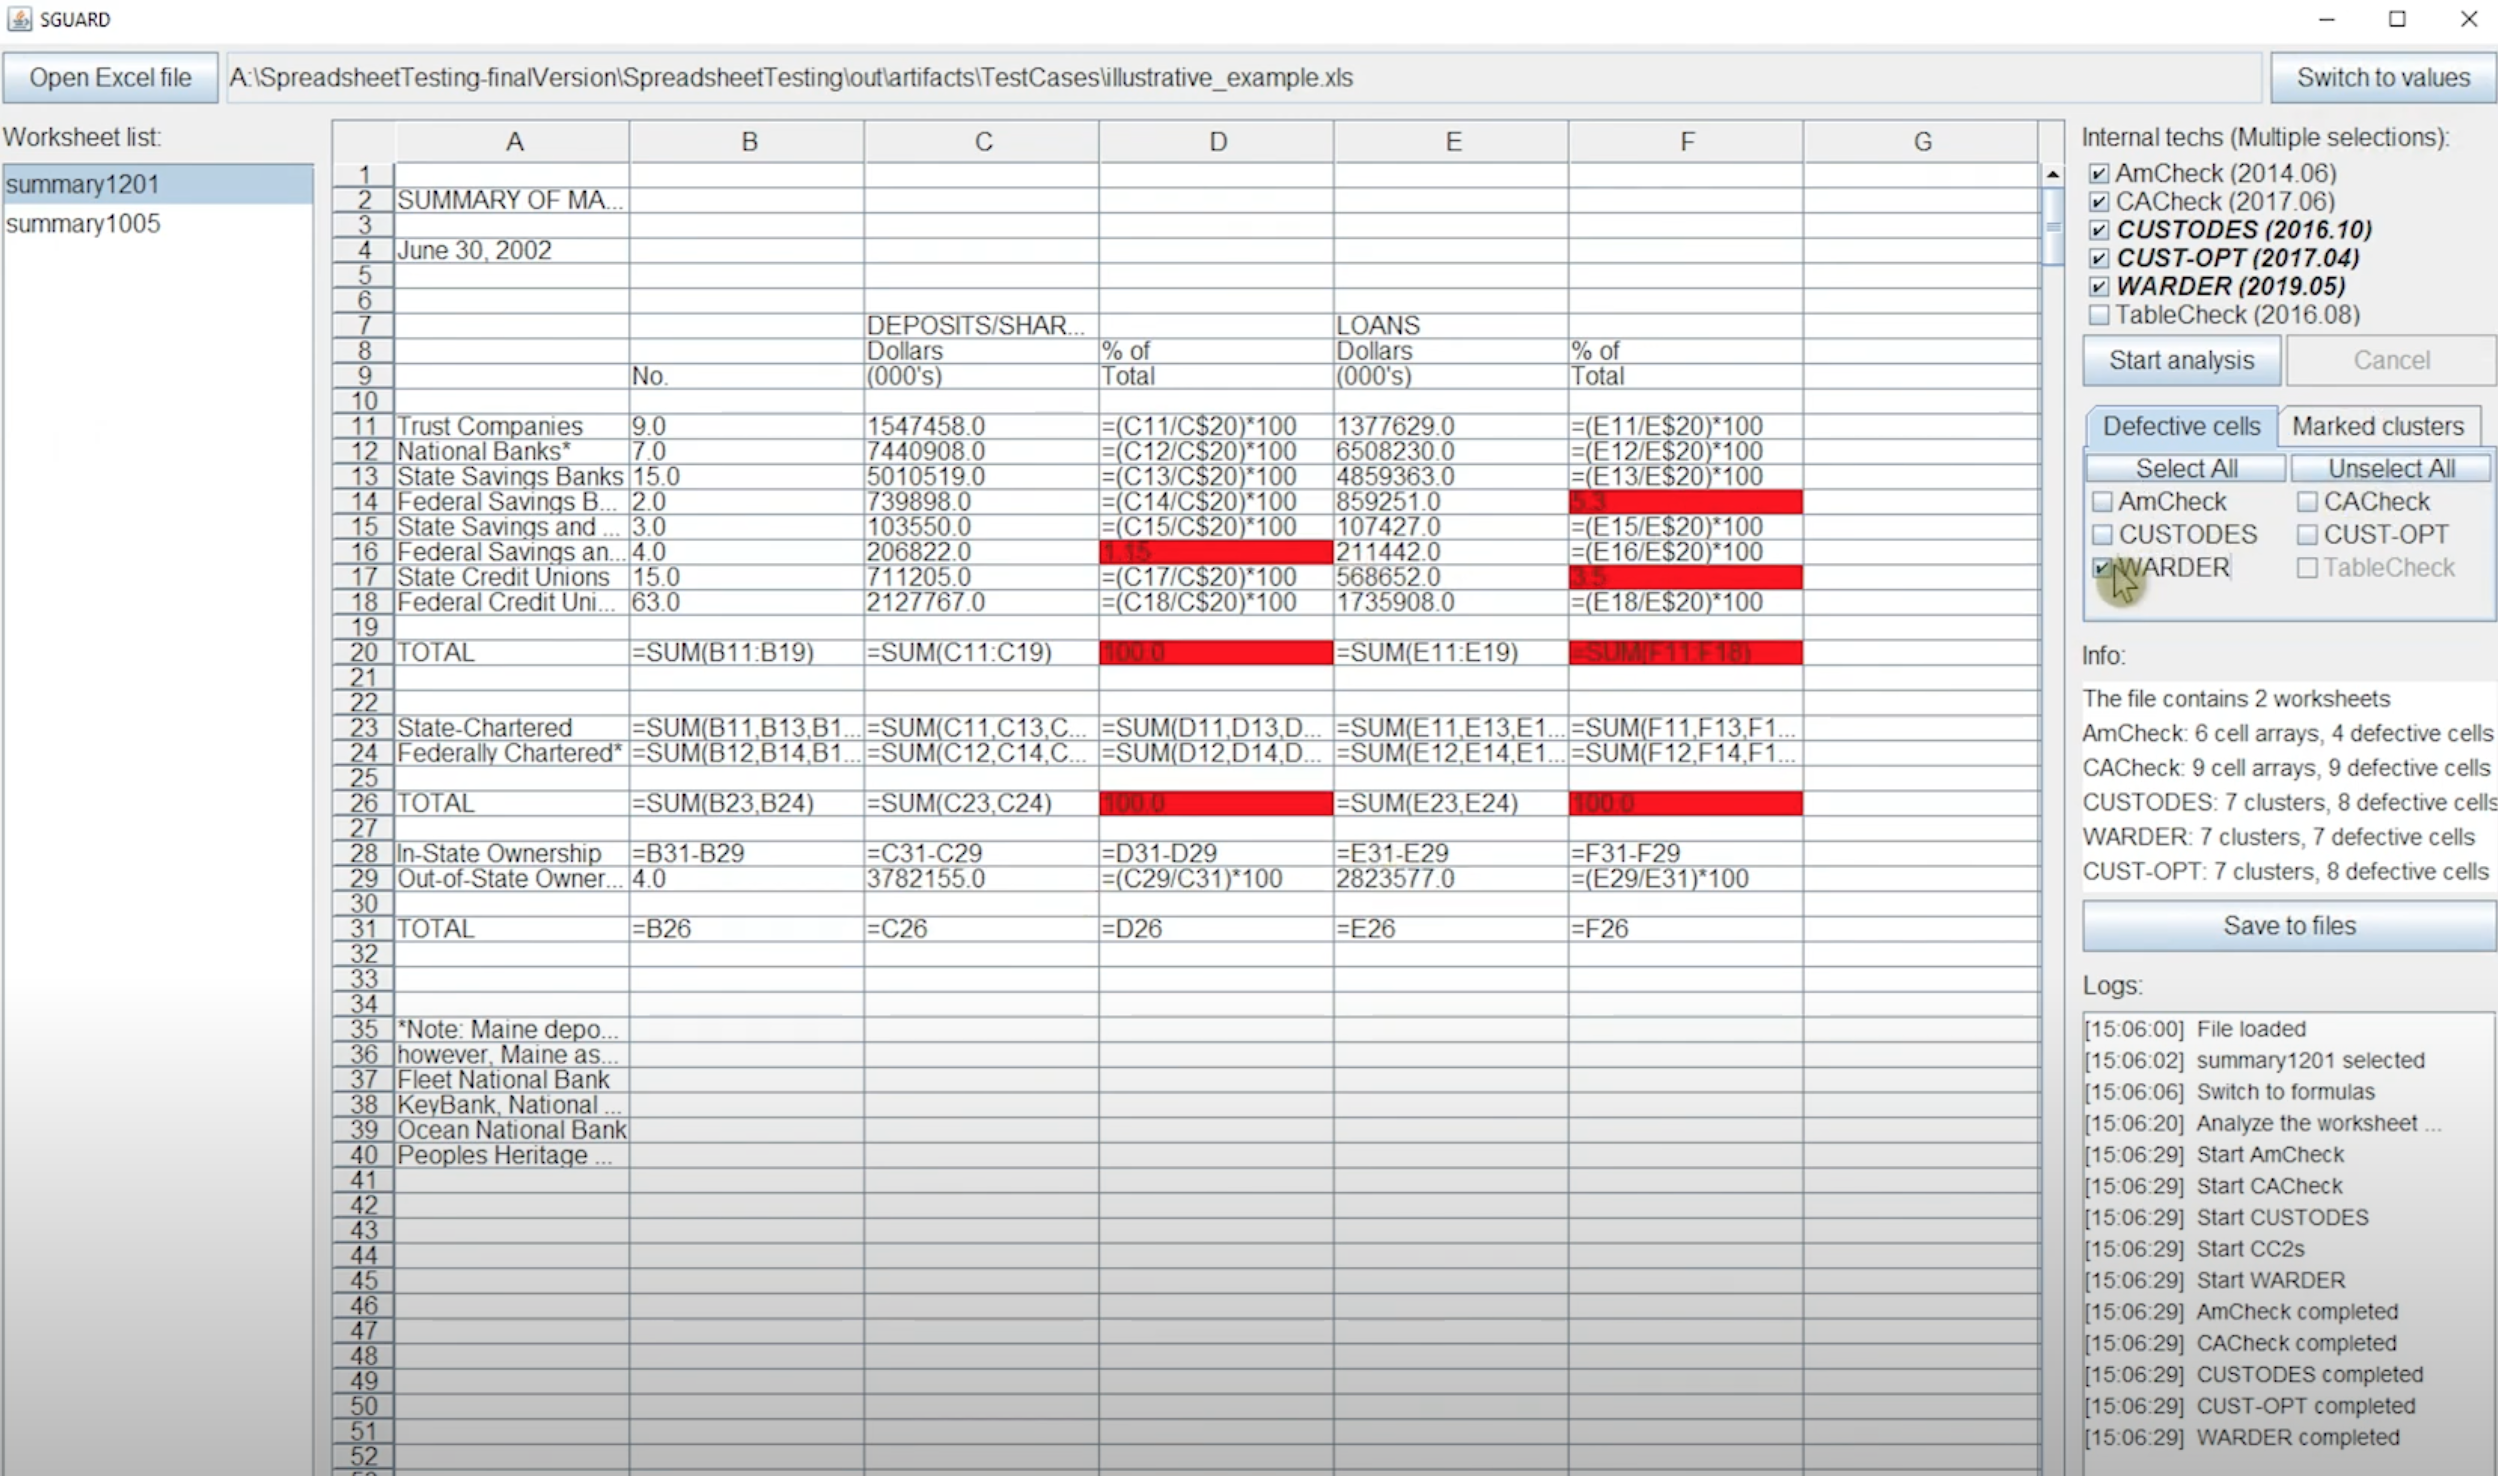
\includegraphics[width=\textwidth]{figure/sg/sguard-5.png}
    \caption{\sg 的使用流程演示截图 5}
    \label{figure-sg5}
\end{figure}
\begin{figure}[tbp]    
    \centering
    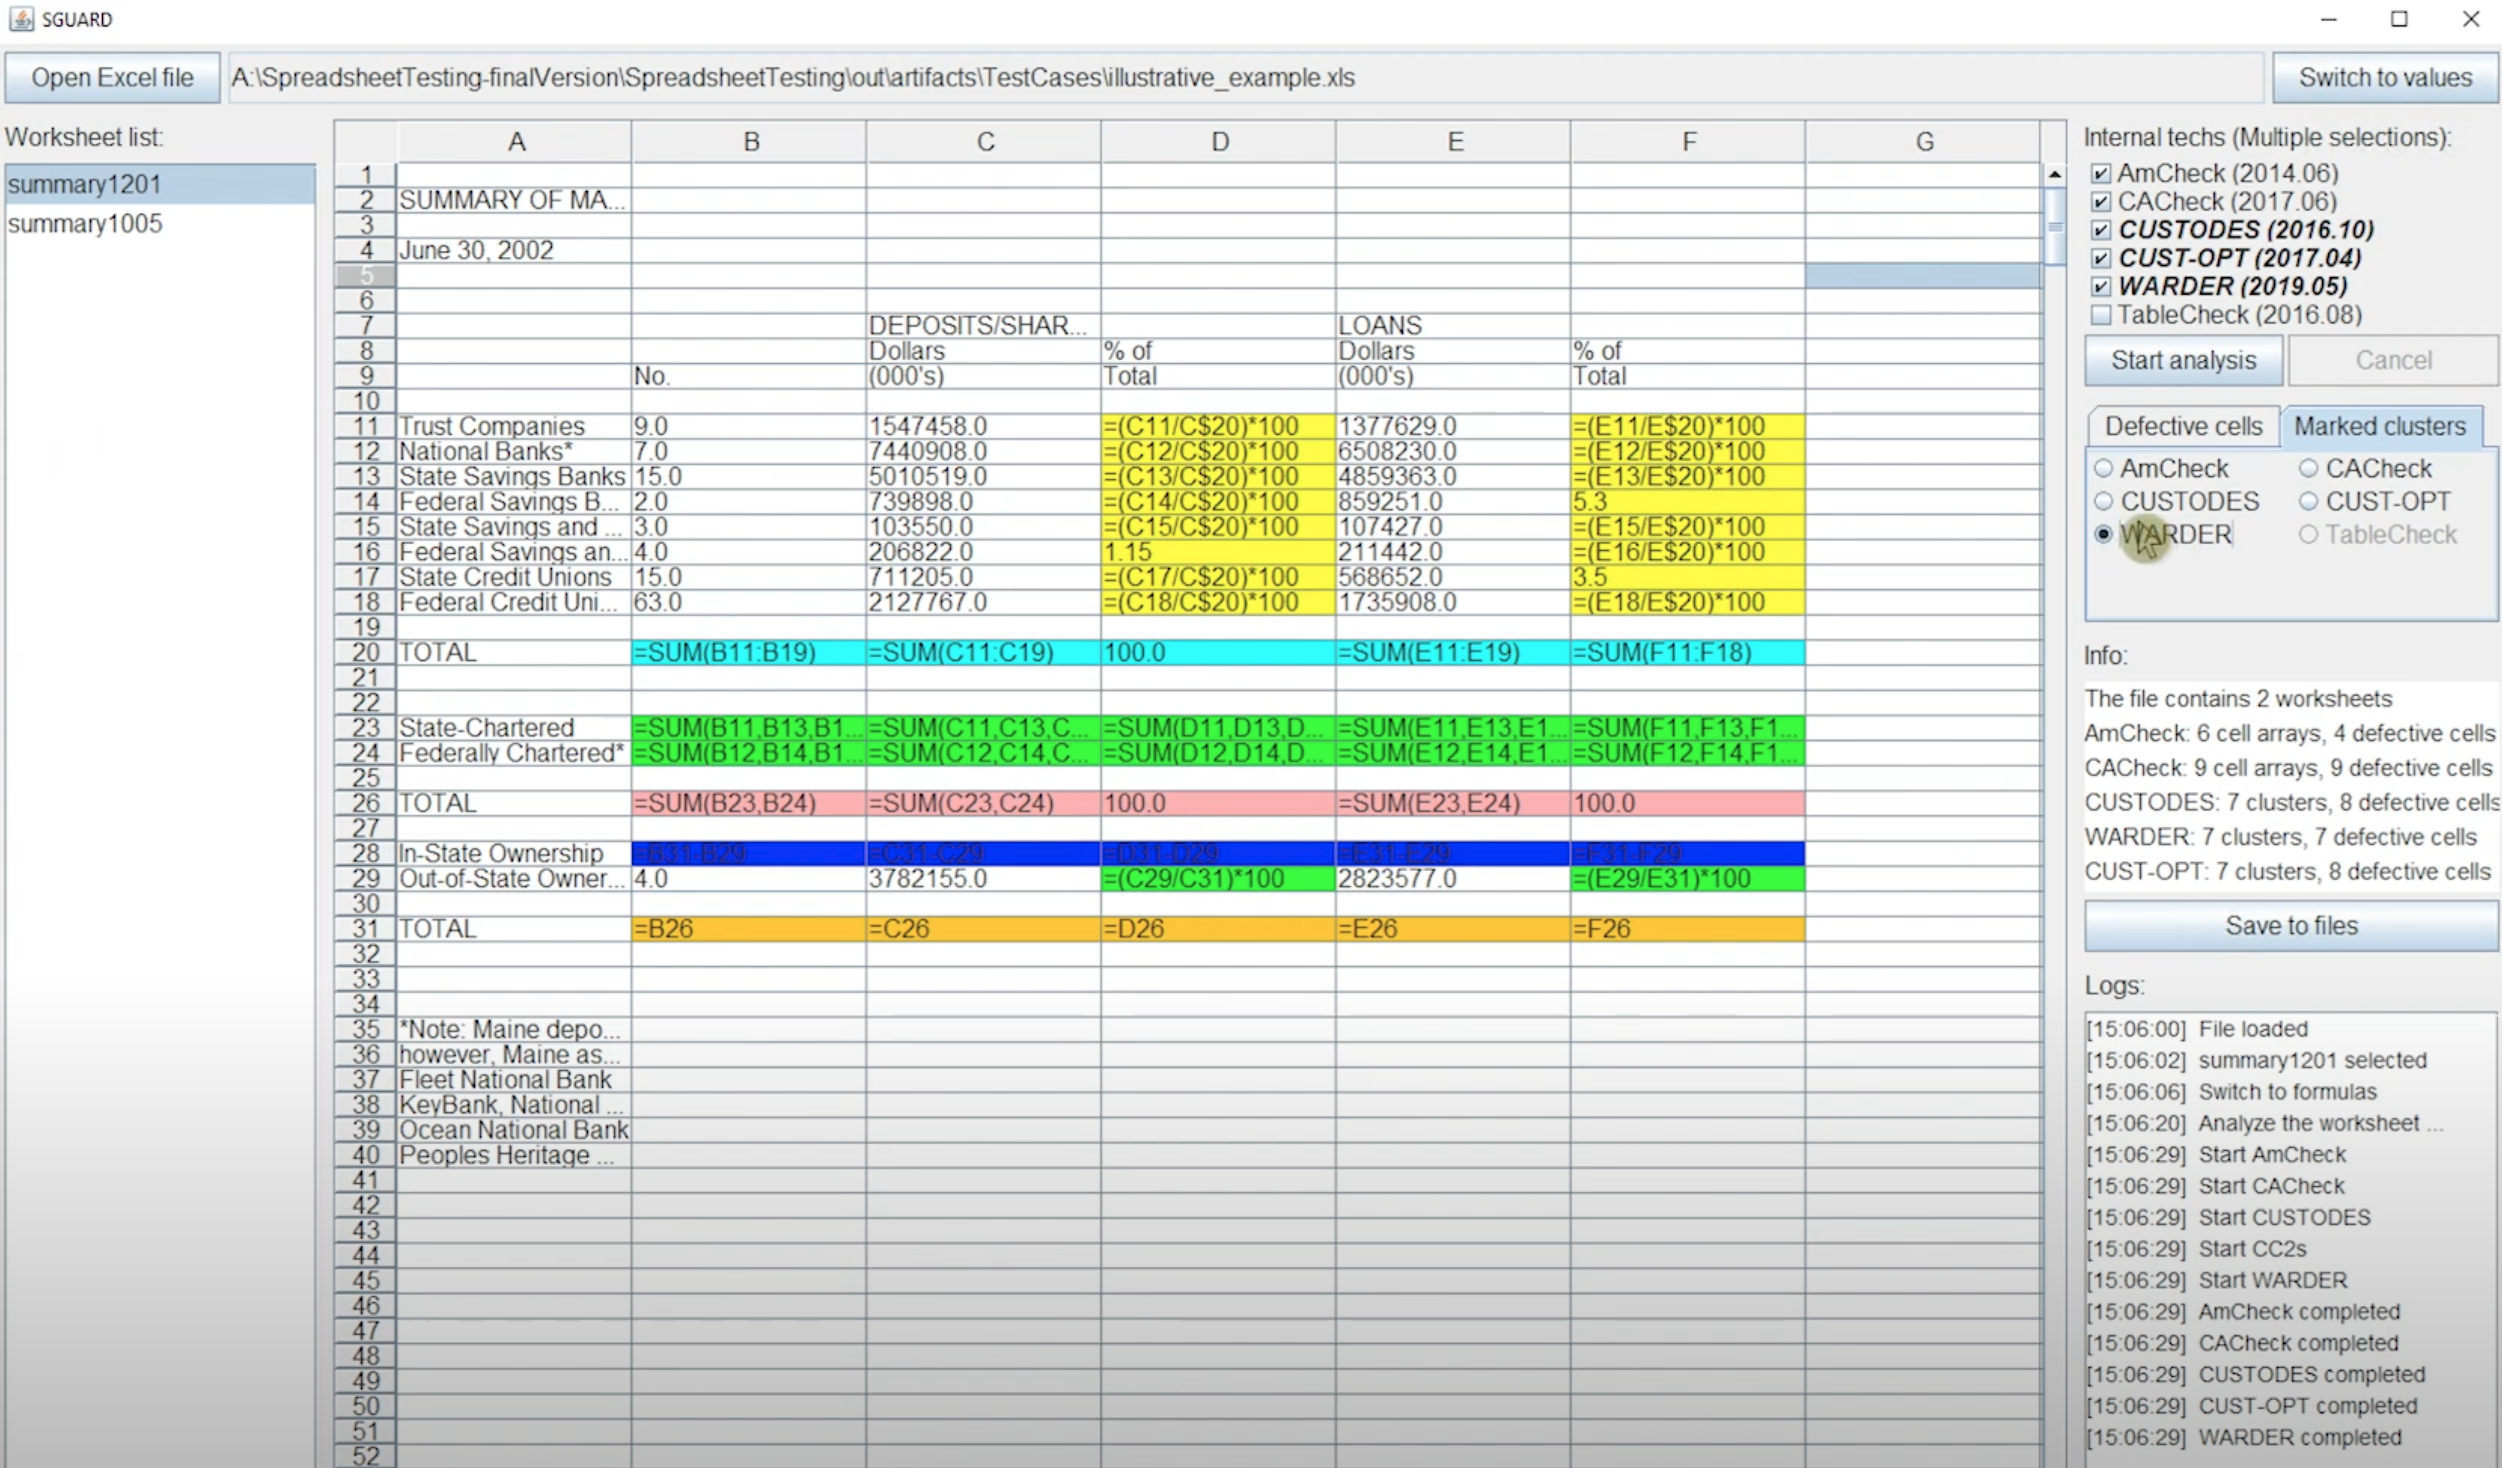
\includegraphics[width=\textwidth]{figure/sg/sguard-6.png}
    \caption{查看 \wa 技术的单元格聚类结果}
    \label{figure-sg6}
\end{figure}
% \begin{figure}[tp]    
    \centering
    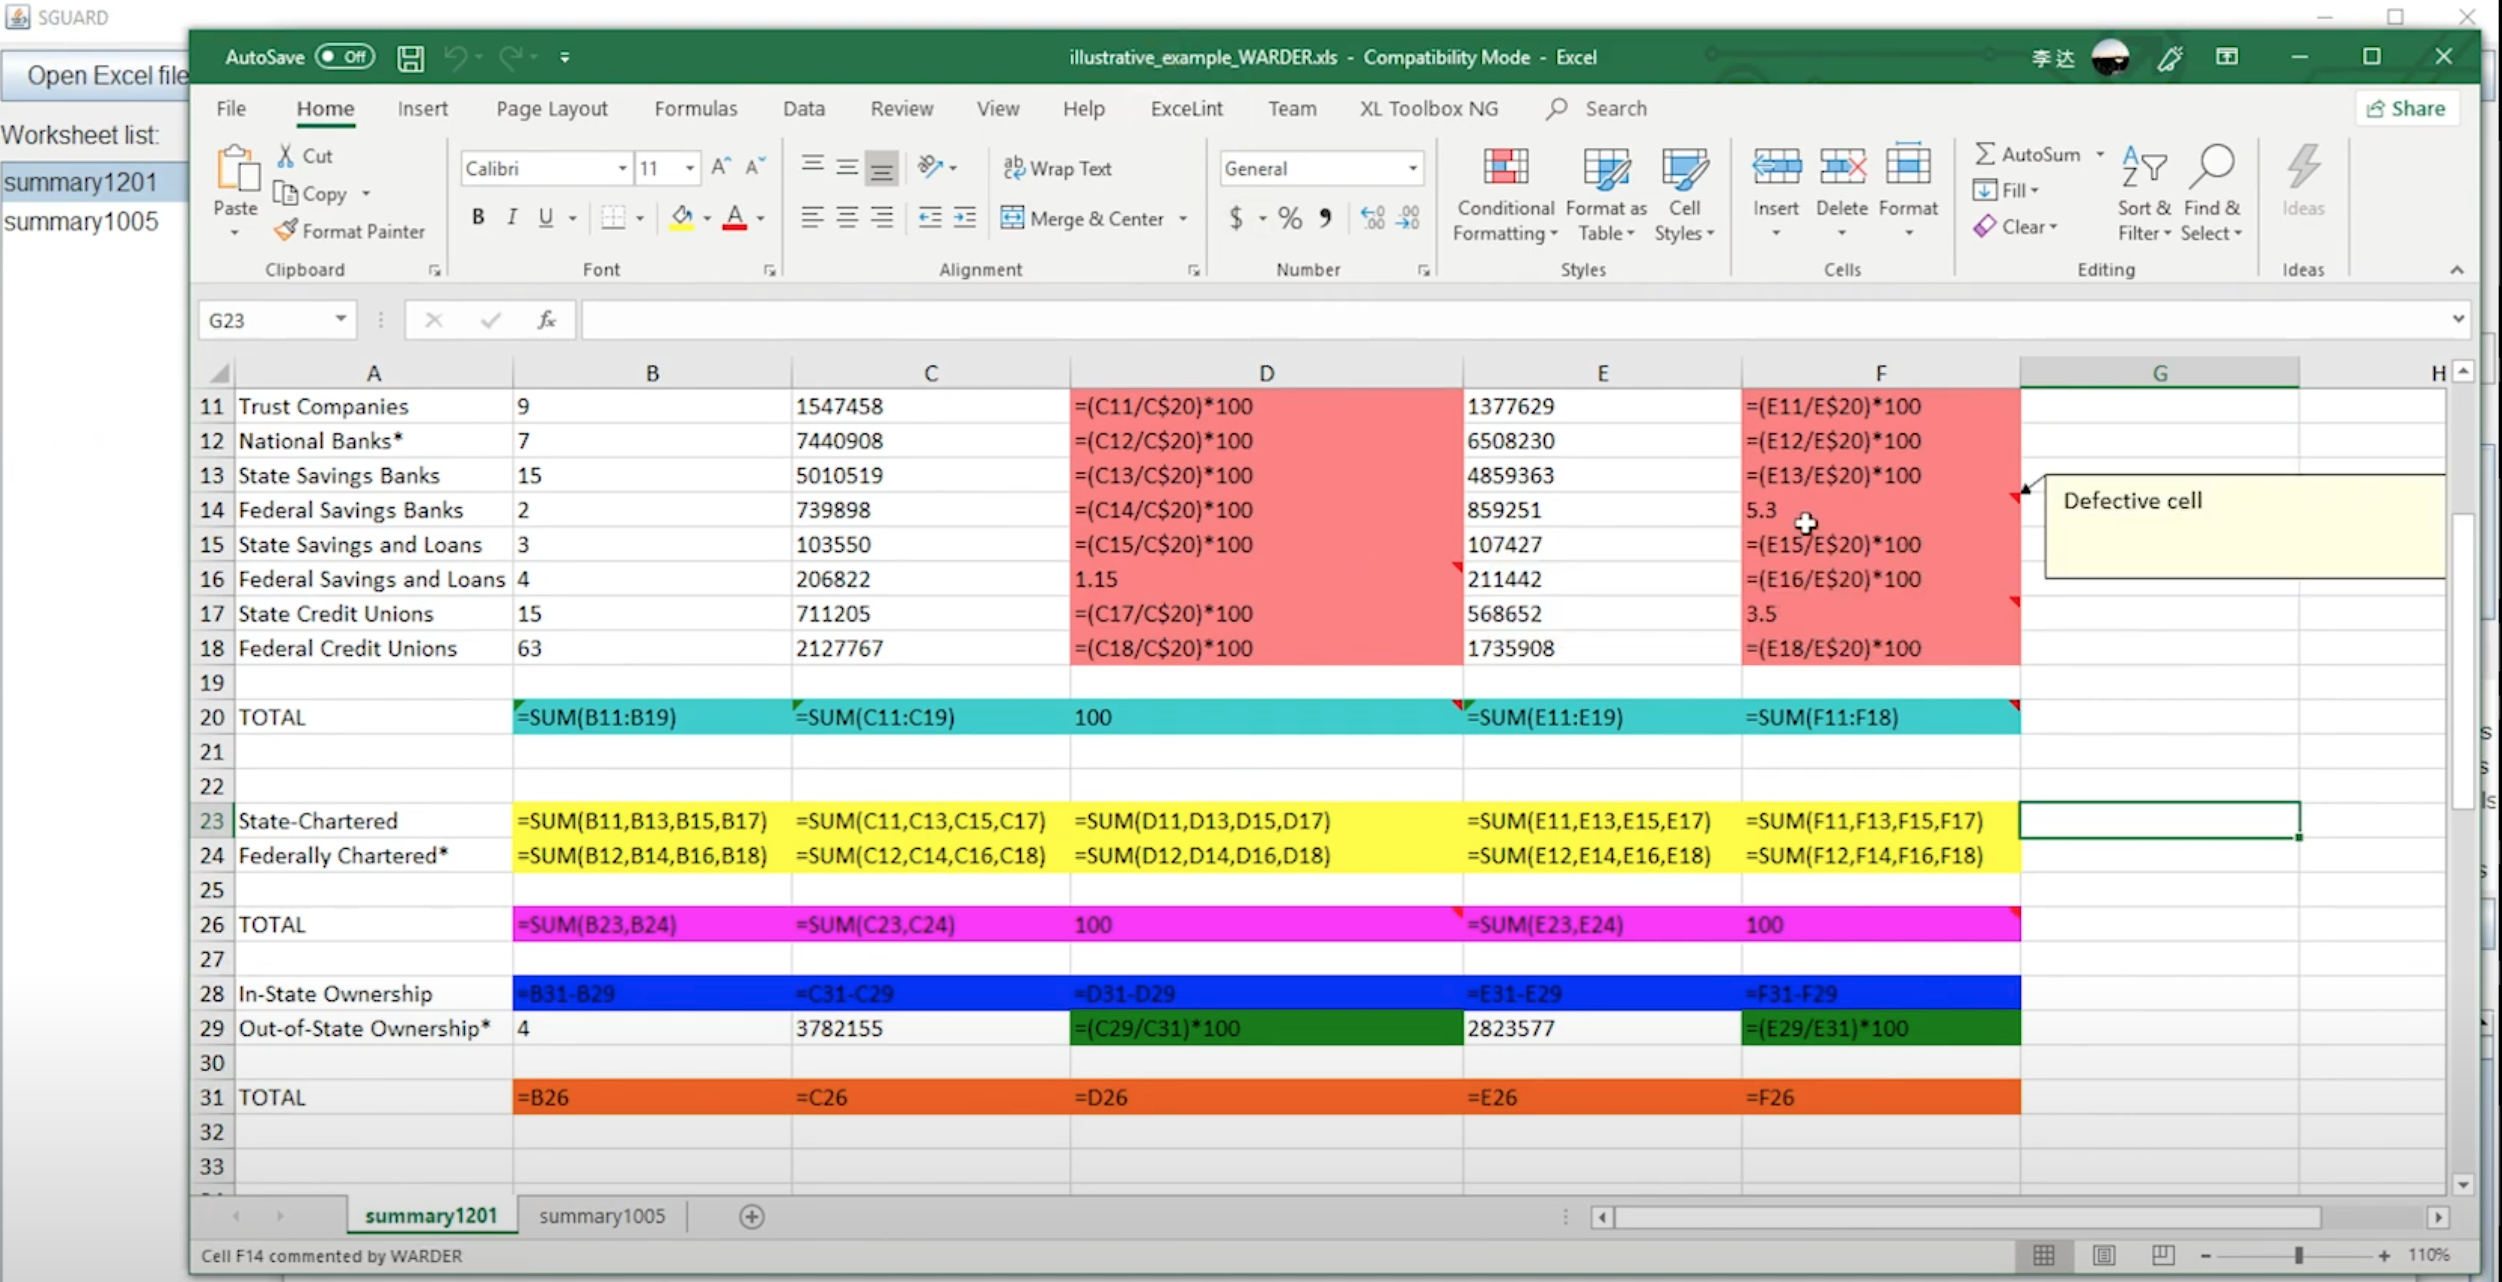
\includegraphics[width=\textwidth]{figure/sg/sguard-8.png}
    \caption{在 Excel 中查看保存好的 \wa 检测结果}
    \label{figure-sg8}
\end{figure}
图\ref{figure11} 展示了\sg 使用交互界面来检测电子表格缺陷并展示相应结果的截图。
整个界面包含四大区域:

\begin{itemize}
    \item 上方的文件选取区域包含 Open Excel file(打开 Excel 文件)和Switch to values/formulas(切换到数值/公式形式)两个按钮,中间部分显示当前打开的 Excel 文件路径;
    
    \item 左侧的工作表选择区域列出了当前选定的 Excel 文件的所有工作表;
    
    \item 中间的工作表内容展示区域展示了类似于电子表格软件的核心界面,即以字母标记的列号(A,B,\dots)和以数字标记的行号(1,2,\dots),每个对应的表格位置显示该工作表的具体内容,即公式、数值或文本,目前不能显示除此以外的内容,比如工作表中插入的图,以及不会保留原工作表的排版风格,只显示每个单元格里的具体内容;
    
    \item 右侧的核心操作区域包含如下几块内容:

        \begin{enumerate}
            \item 上方罗列了 \sg 工具内部囊括的所有检测技术,共有 6 个检测技术,分别是 \am\cite{dou2014spreadsheet},\ca\cite{dou2017cacheck},\cu\cite{cheung2016custodes},\cu-OPT\footnote{http://sccpu2.cse.ust.hk/custodes/cc2s.html},\wa 和 TableCheck\cite{dou2016detecting}。每个技术名称后面标记了对应论文发表的时间或者该技术更新的最新时间;
            
            \item 紧接着向下是 Start analysis 和 Cancel 两个按钮,分别用来开始执行技术对应的代码和取消当前分析过程;
            
            \item 再往下有两个标签,Detective cells 和 Marked clusters,每个运行的技术分别对应标签内部的一个选项;
            
            \item 再往下是 Info 栏,展示一些执行信息以及每个电子表格缺陷检测结果汇总,包含每个技术检测到的单元格类数量和有缺陷的单元格数量;
            
            \item 紧接着是一个 Save to files 按钮,可以用来保存当前选定技术的检测结果到新的 Excel 文件中;
            
            \item 最后是 Logs 栏,用来显示每个完成执行的技术和对应的时间戳。
        \end{enumerate}

\end{itemize}

\subsection{使用展示}
接下来,我们结合一个具体的工作表来展示 \sg 的完整使用流程。

\begin{enumerate}
    \item 我们点击 Open Excel file 按钮,从文件浏览器中选择一个要测试的电子表格,这里我们选择一个电子表格文件illustrative\_example.xls;
    
    \item 如图\ref{figure-sg4}所示,从左侧列出的工作表中,我们选择名为 summary1201 的工作表,对应的单元格内容就自动显示在正中间;
    
    \item 如图\ref{figure-sg4}所示,我们在右侧功能区选择准备使用的电子表格测试技术,这里我们勾选上除 TableCheck 之外的所有技术,并点击 Start analysis 开始执行;
    
    \item 如图\ref{figure-sg5}所示,我们会在 Logs 区域看到各个技术开始和结束的标志,在 Defective cells 选项卡里可以勾选上多个技术,查看对应检测到的缺陷单元格全集,这里我们选择 \wa 技术,可以看到 \wa 检测到了 7 个缺陷单元格,与 Info 区域显示的检测结果保持一致;
    
    \item 如图\ref{figure-sg6}所示,我们在 Marked clusters 选项卡里也可以勾选多个技术,这里我们选择\wa 技术,中间区域显示出\wa 检测到的 7 个单元格类,与 Info 区域显示的检测结果保持一致;
    
    \item 我们点击 Save to files 按钮之后,每个技术的检测结果单独生成一个 Excel 文件,和源文件放在同一个目录下;
    
    % \item 如图\ref{figure-sg8}所示,
    \item 我们打开 illustrave\_example\_WARDER.xls 文件,顾名思义,该文件记录了 \wa 的检测结果,其中标注了和 \sg 工具中显示的相同的单元格类,以及在右上角用注释的方式标注出有公式缺陷的单元格。
\end{enumerate}


\chapter{实验评估}

本章中,我们评估我们的技术WARDER,并和现有的电子表格缺陷检测技术作对比。

\section{研究问题}

我们旨在回答下列三个研究问题:

\begin{itemize}
    \item \textbf{研究问题1(有效性)}:与现有电子表格缺陷检测技术相比,\wa 在单元格聚类和缺陷检测方面有效性如何?
    \item \textbf{研究问题2(相关性)}:\wa 优化后的单元格聚类对最终的缺陷检测精度提升有多大贡献?
    \item \textbf{研究问题3(独立性)}:\wa 的三个有效性精化方法对缺陷检测的效果提升分别有多大?
\end{itemize}

\section{实验设计和设置}
\begin{table}[tbp]
    \centering
    \caption{基准测试集的统计数据}
    \label{table1}
    %\large
    \resizebox{\columnwidth}{!}{
    \begin{tabular}{|m{.15\columnwidth}<{\centering}|m{.12\columnwidth}<{\centering}|m{.15\columnwidth}<{\centering}|m{.2\columnwidth}<{\centering}|m{.15\columnwidth}<{\centering}|m{.25\columnwidth}<{\centering}|}
    \hline
    \textbf{\# 电子表格} &  \textbf{\# 工作表} &  \textbf{\# 单元格} &  \textbf{\# 公式单元格} &  \textbf{\# 单元格类} &  \textbf{\# 有缺陷的单元格} \\ 
    \hline
    70 & 291 & 189,027 & 26,716 & 1,610 & 1,974 \\
    \hline
    \end{tabular}}
\end{table}

\subsection{系统实现}
\wa 技术在实验评估中使用 Java 语言实现,并使用 Apache POI 库 \footnote{https://poi.apache.org} 来读写 Excel 格式的电子表格。
相应源码发布在 GitHub 网站上 \footnote{https://github.com/dlee992/QRS19-Code} 。

\wa 工具总共包含约 7,300 行 Java 代码,除了包含 \cu 的源代码以外,额外增改了约 2,500 行代码。
类似于 \cu 的方式,\wa 标记它分析过的电子表格的方法是使用不同的背景色来标注检测到的同一张工作表内的所有单元格类,并通过在单元格右上角添加注释的方式标注含有公式缺陷的单元格的备注信息,包括所在类的信息和具体的公式缺陷种类。

\subsection{基准测试集} 
为了便于 \wa 和它的前身 \cu 进行比较,我们选择了 \cu 使用的采样自EUSES数据库的70 个电子表格,作为本文的实验基准测试集。
如表~\ref{table1}所示,该测试集包含 70 个电子表格和 291 个工作表。这 291 个工作表包含 189,027 个单元格,其中包含 26,716 个公式单元格。
出于实验评估的目的,该测试集额外包含人工标注的数据(标注的方法详见~\cite{cheung2016custodes}),其中包含 1,610 个单元格类和 1,974 个有公式缺陷的单元格。

\subsection{测试技术} 
在实验中, \wa 将和 5 个之前提到的电子表格缺陷检测技术进行对比,即 \uc、\di、\am、\ca 和 \cu 。
我们从它们各自的原作者那里获取了对应的可执行工具或源码。
除了 \ca 以外,其它技术的方法中并没有单元格类的概念,因此我们主要在缺陷检测的有效性方面对这些技术进行比较。
对于\ca,我们额外比较了它和 \wa 的单元格聚类的有效性。

为了评估三个有效性检验方法的独立性(研究问题3),我们采用不同的配置来测试各自的实验效果,三种配置依次分别标记为 \wasc (含有针对单个单元格自身的有效性检验方法),\wamc (含有针对单元格之间关系的有效性检验方法),\wawc (含有针对整个类的有效性检验方法)。
最后,带有全部三种检验的配置被称为 \wa-full,简记为 \wa 。

\subsection{评价指标} 
为了衡量缺陷检测的有效性,我们首先统计每个技术检测出的缺陷数量,以及其中的真阳性($TP$),假阳性($FP$)和假阴性($FN$)数量。
基于此,我们进一步根据如下三组公式计算精度 $precision_d$、召回率 $recall_d$ 和 $F\text{-}measure_d$ 值\cite{yoshida2010person},来衡量电子表格缺陷检测上各技术的有效性。

\begin{gather*}
    precision_d=\frac{TP}{TP + FP}\qquad recall_d = \frac{TP}{TP + FN}\\
    f\text{-}measure_d = \frac{2 * precision_d * recall_d}{precision_d + recall_d}
\end{gather*}

针对电子表格缺陷的有效性(适用于 \wa 和 \cu),我们采用和 \cu 类似的方式来统计真阳性($TP$),假阳性($FP$)和假阴性($FN$)数量\footnote{限于篇幅原因,具体统计方式可参考\cite{cheung2016custodes}第 6.2 节}。
类似地,我们也计算出这两个技术在单元格聚类上的精度 $precision_c$,召回率 $recall_c$和 \fmc 值。

\subsection{测试环境} 
所有实验在一台台式机上进行,配有 Intel$^\circledR$ Core\texttrademark\ i7-6700 CPU @3.41GHz 处理器和 64GB 内存。该机器上安装了微软 Windows 10 专业版操作系统和 Oracle Java 8 执行环境。


\section{实验结果和分析}

本节中,我们会依次分析实验结果并回答上述提出的三个研究问题。

\subsection{有效性}

我们首先实验评估\wa 在单元格聚类和缺陷检测方面的有效性,然后和其他五个电子表格缺陷检测技术的结果进行比较。

\begin{table}[tbp]
    \centering
    \caption{6个电子表格缺陷检测技术的检测结果}
    \label{table2}
    \large
    \resizebox{\columnwidth}{!}{
    \begin{tabular}{|c|c|c|c|c|c|c|}
    \hline
    \textbf{技术} & \textbf{检测出} & \textbf{TP} & \textbf{FP} & \textbf{$precision_d$} & \textbf{$recall_d$} & \textbf{$F\text{-}measure_d$} \\
    \hline
        UCheck & 204 & 1 & 203 & 0.5\% & 0.1\% & 0.00 \\
    \hline
        Dimension & 1,824 & 14 & 1,828 & 0.8\% & 0.7\% & 0.01 \\
    \hline
        AmCheck & 2,372 & 1,316 & 1,030 & 56.1\% & 66.7\% & 0.61 \\
    \hline
        CACheck & 1,866 & 1,350 & 516 & 72.3\% & 68.4\% & 0.70 \\
    \hline
        CUSTODES & 2,380 & 1,539 & 841 & 64.7\% & 78.2\% & 0.71 \\
    \hline
        WARDER & 1,612 & 1,415 & 197 & 87.8\% & 71.9\% & 0.79 \\
    \hline
    \end{tabular}}
\end{table}

就缺陷检测而言,表~\ref{table2}对比了所有6个检测技术的结果,包括精度,召回率,\fmd,检测出的缺陷数量,以及其中包含的真阳性和假阳性。从表中,我们观察到:

\begin{enumerate}
    \item 由于他们有限的分析范围,\uc 和\di 获得了较低的分数(精度和召回率都低于1\%,\fmd 值也仅有0.01),这点也与之前的实证研究结果~\cite{zhang2017effectively}保持一致;
    \item 由于他们有效的分析模式(比如,单元格元组),\am 和 \ca 获得了较好的分数(56.1-72.3\%的精度,66.7-68.4\%的召回率,以及0.61-0.70的\fmd 值);
    \item \cu 比 \ca 获得了略微更好地分数(0.71的\fmd 值),以及对召回率的较大提升(72.8\%,对应的\ca 召回率为68.4\%);
    \item 如同预期的那样,\wa 关注于提升检测精度,对比于\cu 获得了大幅度提升,从64.7\% 提升到 87.8\%,最终总体上提升了\fmd 的值,从0.71到0.79,尽管对召回率有6\%的牺牲。 从数据中,可能产生一定疑惑:\cu 比 \wa 多检测出124个真阳性,但同时伴随着更多的假阳性(达644个),这对于终端用户的人工验证来说是很大的负担。
\end{enumerate}

\begin{figure}%
    \centering
    \subfloat[精度比较(仅展示被影响的工作表)]{{
        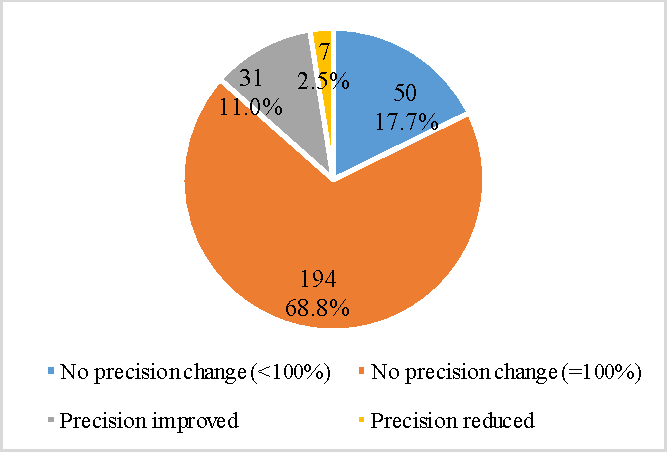
\includegraphics[width=0.40\textwidth]{figure/figure5a.pdf} 
        \label{figure5a}
        }}%
    \subfloat[召回率比较(整体)]{{
        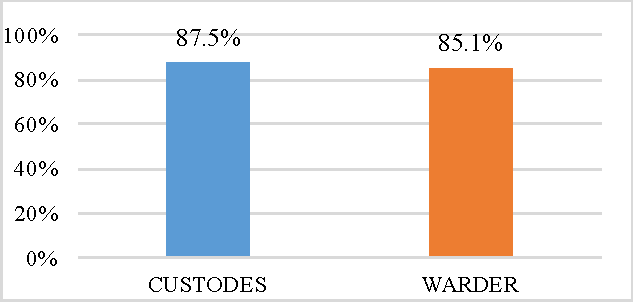
\includegraphics[width=0.55\textwidth]{figure/figure5b.pdf} 
        \label{figure5b}
        }}%
    \caption{CUSTODES 和 WARDER 的单元格聚类结果}%
    \label{figure5}%
\end{figure}

就单元格聚类而言,图\ref{figure5}比较了\cu 和 \wa 在精度和召回率两方面的结果。从精度比较来看(如图\ref{figure5}(a)),我们把包含至少有一个单元格类的282个工作表分成两类:
\begin{enumerate}
    \item \wa 提升了其中31个工作表的精度,降低了7个;
    \item 对于余下精度保持不变的244个工作表,其中194个已达到100\%(即上限)。
\end{enumerate}
换言之,\wa 提升了225个工作表的单元格聚类精度,要么是实际提升精度,要么已经达到上限。如图\ref{figure6}所示,我们进一步观察这38个精度产生变化的工作表。我们不难发现,\wa 在不同程度上提升了单元格聚类的精度(0.3\%-94.6\%,平均20.7\%),这样的精度提升是显著的,远多于精度受损的部分。另外从图\ref{figure5}(b)中,我们也注意到,\wa 在精度提升上的有效性也仅导致召回率的轻微下降(2.4\%)。

\begin{figure*}
    \centering
    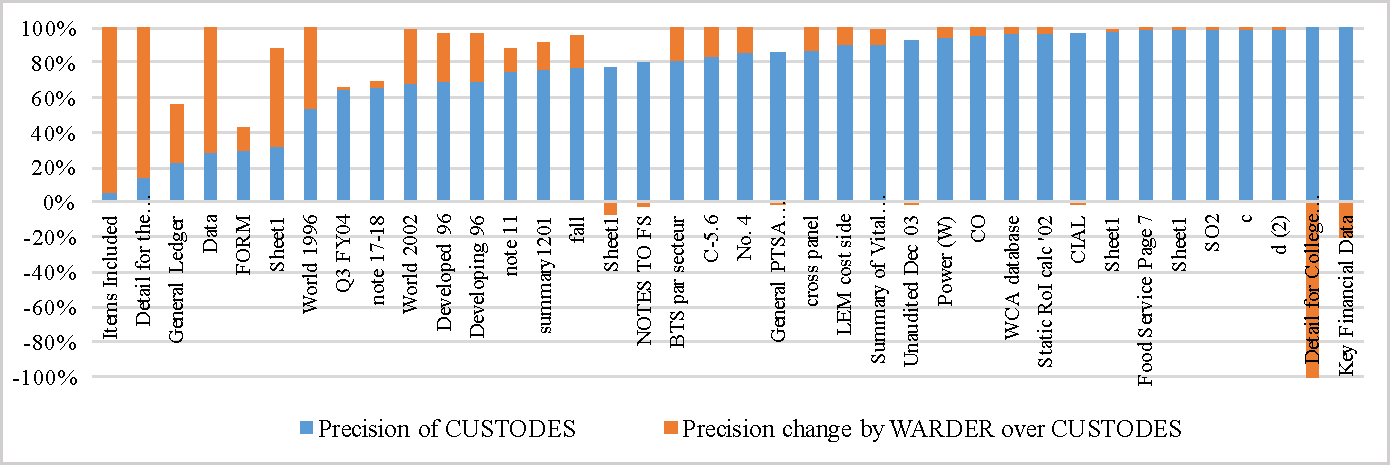
\includegraphics[width = \columnwidth]{figure/figure6.pdf}
    \caption{CUSTODES 和 WARDER 的单元格聚类结果(精度变化方面)}
    \label{figure6}
\end{figure*}
\begin{figure}[tp]
    \centering
    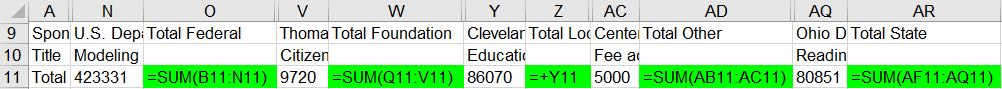
\includegraphics[width = \columnwidth]{figure/figure7.jpeg}
    \caption{工作表“Detail for College of Education” (包含一个绿色标记的单元格类)}
    \label{figure7}
\end{figure}

如图~\ref{figure6}所示,我们也观察到,\wa 对大多数精度受影响的工作表是正面作用,但也有极少量的例外情况,如名为“Detail for College ...”的工作表,它的聚类精度从100\%降低到了0。因此,我们进一步检查了该工作表的聚类情况。如图\ref{figure7}所示,人工标记的结果是,{O11,W11,Z11,AD11,AR11}应该被安排在同一个类中。\cu 看似正确地对这些单元格进行了分类,而\wa 分类得很差。然而,我们发现这五个单元格实际上包含不同的公式,因此它们违反了\wa 的 \wcvp (在这些单元格中不存在一个公共的计算语义能够覆盖过半数量)。事实上,这个单元格类的确不包含任何缺陷。因此,这个单元格聚类精度下降的案例并不影响\wa 的缺陷检测能力。

因此,针对研究问题1,我们能够得出如下结论:\textit{\wa 在单元格聚类和缺陷检测方面是有效的。它极大地提升了精度,达15.5-87.3\%,并且在所有被比较的电子表格缺陷检测技术中,取得了最佳的 \fmd 值(0.79)。}

\subsection{相关性}

\begin{table}[tbp]
    \centering
    \caption{\wa 相对于 \cu 在单元格聚类和缺陷检测上的的精度变化 ($\uparrow$: 精度提升, $\downarrow$: 精度下降, $\to$: 精度保持不变)}
    \label{table3}
    %\Large
    \begin{tabular}{|m{.16\columnwidth}<{\centering}|m{.16\columnwidth}<{\centering}|m{.16\columnwidth}<{\centering}|m{.08\columnwidth}<{\centering}|m{.18\columnwidth}<{\centering}|}
    \hline
    \textbf{相关性类型} & \textbf{聚类的精度变化} & \textbf{缺陷检测的精度变化}  & \textbf{\# 工作表} & \textbf{总计} \\
    \hline
        \multirow{3}{1.2cm}{正相关} & $\uparrow$  & $\uparrow$ & 8 & \multirow{3}*{126 (90.0\%)}\\
    \cline{2-4}
        ~ & $\downarrow$ &  $\downarrow$  & 2 & ~\\
    \cline{2-4}
        ~ & $\to$ &  $\to$  & 116 & ~\\
    \hline
            \multirow{4}{1.2cm}{负相关}& $\uparrow$ &  $\to$  & 5  & ~\\
    \cline{2-4}
         ~ & $\uparrow$  & $\downarrow$ & 2 & \multirow{4}*{9 (6.4\%)}\\
     \cline{2-4}

        ~ & $\downarrow$ &  $\to$  & 2 & ~ \\
    \cline{2-4}
        ~ & $\downarrow$ &  $\uparrow$  & 0 & ~ \\
    \hline
    \multirow{2}*{不相关} & $\to$  & $\uparrow$ & 5 & \multirow{2}*{5 (3.6\%)}\\
    \cline{2-4}
        ~ & $\to$ &  $\downarrow$  & 0 & ~ \\
    \hline
    合计 & - & - & 140 & 140 (100.0\%) \\
    \hline
    \end{tabular}
\end{table}

在这一小节里,我们研究\wa 相对于 \cu 在单元格聚类和缺陷检测上的的精度提升。

如表\ref{table3}所示,我们用三个符号 $\uparrow$,$\downarrow$和$\to$分别表示精度提升,精度下降,以及精度保持不变这三种情况。按照相关性类型,我们把人工标记中至少含有1个缺陷的工作表分成3个类型:
\begin{enumerate}
    \item \textit{正相关}:当相对于\cu 的单元格聚类,\wa 的精度有提升,下降或不变时,在缺陷检测上精度变化表现一致;
    \item \textit{负相关}:当相对于\cu 的单元格聚类,\wa 的精度有提升时,在缺陷检测上精度下降或保持不变;或者相反地,\wa 的精度下降时,在缺陷检测上精度提升或保持不变;
    \item \textit{不相关}:其他的组合情况,均划归此类,既不表现出正相关,也不表现出负相关。
\end{enumerate}
总得来说,我们能够观察到:第一类占据主导(90\%),因此表明 \wa 对单元格聚类的精度提升方法的确能够带来缺陷检测精度的提升,并且九成比例成明显正相关。

\begin{figure}%
    \centering
    \subfloat[CUSTODES 和 WARDER 在单元格聚类上的精度]{{
        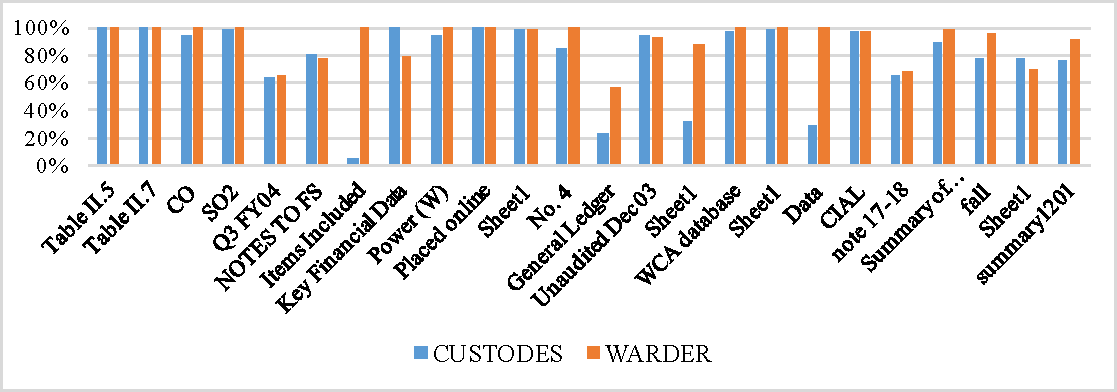
\includegraphics[width=.95\columnwidth]{figure/figure8a.pdf} 
        \label{fig8a}
        }}%
    \qquad
    \subfloat[CUSTODES 和 WARDER 在缺陷检测上的精度]{{
        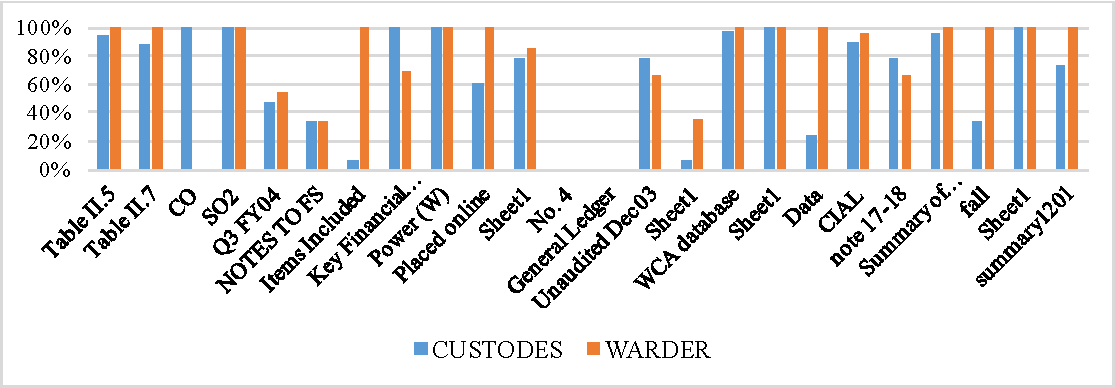
\includegraphics[width=.95\columnwidth]{figure/figure8b.pdf} 
        \label{fig8b}
        }}%
    \caption{\cu 和 \wa 中有精度变化的工作表}%
    \label{figure8}%
\end{figure}
\begin{figure}[tbp]
    \centering
    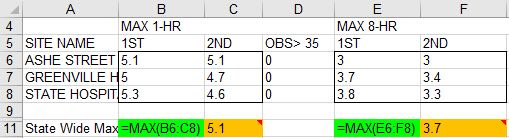
\includegraphics[width = .95\columnwidth]{figure/figure9.jpg}
    \caption{工作表 ``CO'' (两个类分别用绿色和橙色标记)}
    \label{figure9}
\end{figure}

图\ref{figure8}展示了在单元格聚类和缺陷检测上\wa 和 \cu 的更细致的精度对比。为了展示的清晰性和简洁性,我们移除了精度前后无变化的 116 个工作表,仅罗列出剩下的 24 个。细致的观察可以发现:在单元格聚类和缺陷检测的精度变化上大部分情况下是正相关的。不过,其中一个例外是名为“CO”的工作表,在这张表上,\wa 的缺陷检测精度从100\%跌至 0,然而单元格聚类精度却有提升。我们进一步检查了这个情况。如图\ref{figure9}所示,人工认为单元格{B11,E11}(绿色标记) 和{C11,F11}(橙色标记)应该构成两个类,并且单元格 C11 和 F11 应该是两个缺陷(用红色三角标记)。\cu 因为意外地将这四个单元格分成同类,而偶然地检测到了这两个缺陷。这是偶然的,因为这四个单元格本质上并不共享相同的计算语义(两个绿色的单元格用来计算最大值,而两个橙色的单元格用来计算第二大值)。\cu 只是简单地将两个橙色的单元格标记为缺陷,因为他们仅仅包含纯数值(丢失公式的缺陷)。另一方面,\wa 仅仅将{B11,E11}划分为同一类,因此无法检测到其中的任何缺陷。它漏掉了两个橙色单元格,因为它们不包含任何公式,且没有和它们相同计算语义的公式存在,因而无法被识别到任何类中。当没有额外的证据时(例如,更多的计算第二大值的单元格出现,并且相应的公式也存在于某些单元格中),\wa 选择不把这些单元格放到任何类中(否则,可能导致更多的假阳性)。

因此,针对研究问题2,我们能够得出如下结论:\textit{\wa 在单元格聚类上的改进的确进一步提升了缺陷检测的结果,这一相关性得到90.0\%的工作表的数据支撑。}


\subsection{独立性}

\begin{table}[tbp]
    \centering
    \caption{\cu 和 \wa 在不同配置下的缺陷检测结果}
    \label{table4}
    \large
    \resizebox{\columnwidth}{!}{
    \begin{tabular}{|c|c|c|c|c|c|c|}
    \hline
    \textbf{技术} & \textbf{检测出} & \textbf{TP} & \textbf{FP} & \textbf{$precision_d$} & \textbf{$recall_d$} & \textbf{$F\text{-}measure_d$} \\
    \hline
        CUSTODES & 2,380 & 1,539 & 841 & 64.7\% & 78.2\% & 0.71 \\
    \hline
        WARDER-sc &2,083 & 1,506 & 577 & 72.3\% & 76.3\% & 0.74\\
    \hline
        WARDER-mc &2,164 & 1,507 & 657 & 69.6\% & 76.3\% & 0.73\\
    \hline
        WARDER-wc &2,071 & 1,498 & 573 & 72.3\% & 75.9\% & 0.74\\
    \hline
        WARDER-full & 1,612 & 1,415 & 197 & 87.8\% & 71.9\% & 0.79 \\
    \hline
    \end{tabular}}
\end{table}

最后,我们研究\wa 的三个有效性精化在检测电子表格缺陷上各自的表现。\wa 被配置成单独使用每一种精化方法(正如前面提到的,命名为\wasc,\wamc 和\wawc ),并和同时使用三种方法的\wa 作比较(\wa -full)。

表\ref{table4}对比了\cu 和 \wa 的四种配置的缺陷检测结果。我们可以观察到:
\begin{enumerate}
    \item \wa 的每个有效性精化是有用的,并且各自能够比\cu 在缺陷检测精度上提升 4.9-7.6\%,在召回率上有较小的牺牲(1.9-2.3\%),最终对\fmd 值有小幅提升(从 0.71 提升到 0.73-0.74);
    \item 组合所有三种有效性精化(即\wa -full) 可以获得最高的精度(87.8\%)和\fmd 值(0.79),这也和之前的表\ref{table1}数据相吻合。
\end{enumerate}

因此,针对研究问题3,我们能够得出如下结论:\textit{\wa 的三个有效性属性能够各自独立展现出对缺陷检测的正面效果;同时在三者组合运用时,也能够获得整体的最佳效果。}
\section{案例研究}

\begin{table}[tbp]
    \centering
    \caption{在 VEnron2 数据集上四个电子表格缺陷检测技术的检测结果}
    \label{table5}
    %\large
    \resizebox{\columnwidth}{!}{
    \begin{tabular}{|m{.15\columnwidth}<{\centering}|m{.16\columnwidth}<{\centering}|m{.16\columnwidth}<{\centering}|m{.14\columnwidth}<{\centering}|m{.12\columnwidth}<{\centering}|m{.1\columnwidth}<{\centering}|m{.12\columnwidth}<{\centering}|}
    \hline
    ~& \multicolumn{3}{c|}{\textbf{全部数据集包含 6,258 个工作表}} & \multicolumn{3}{c|}{\textbf{采样 300 个工作表}} \\
    \hline
    \textbf{技术} & \textbf{\# 工作表} & \textbf{\# 缺陷} & \textbf{耗时 (分钟)} & \textbf{\# 缺陷} & \textbf{\# TP} & \textbf{Precision} \\
    \hline
        AmCheck  & 859  & 20,280 & 21 & 3,316 & 540 & 16.3\% \\
    \hline
        CACheck  & 953   & 12,953 & 372 & 1,559 & 534 & 34.3\% \\
    \hline
        CUSTODES & 1,284 & 14,102 & 537  & 2,334 & 629 & 26.9\% \\
    \hline
        WARDER   & 1,136 & 9,462  & 518  & 1,240 & 512 & 41.3\% \\
    \hline
    \end{tabular}}
\end{table}
\begin{figure}[tp]
    \centering
    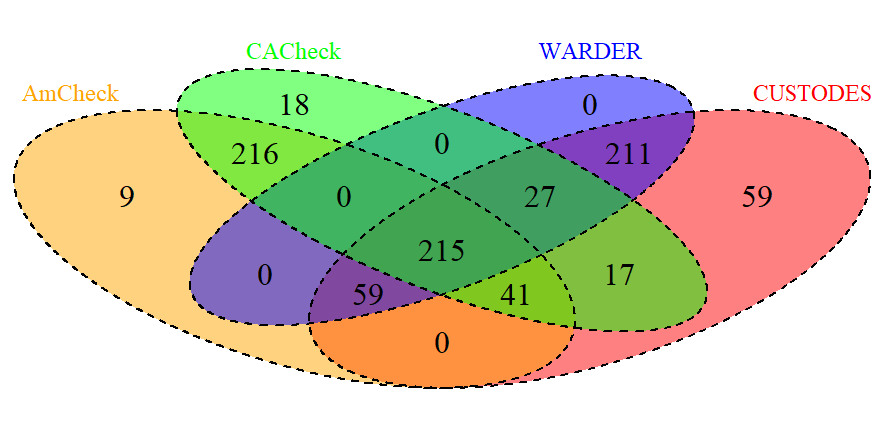
\includegraphics[width = 0.9\columnwidth]{figure/figure10.png}
    \caption{四个电子表格缺陷检测技术报告出的真阳性交集的韦恩图}
    \label{figure10}
\end{figure}



\section{威胁性分析和讨论}

一个主要的内在威胁性来源是单元格聚类有效性的计算方式,即 \prc 、\rec 和 \fmc 。
它们是基于真阳性,假阳性和假阴性概念衍生而来,而后三者又是根据 \cu 的成对相似度~\cite{cheung2016custodes}比较计算而来。
我们注意到该计算过程会统计两个单元格属于同一个类或者属于不同的类的单元格对的数量。
这样的计算方式不同于衡量缺陷检测有效性的方式。
因此,研究 \wa 的单元格聚类和它的缺陷检测相关性结论可能在一定程度上受到影响。
然而,我们依然观察到 90\% 的工作表在我们的分析下是正相关的。
这表明 \wa 对单元格聚类的提升的确有助于最终的缺陷检测。

另外,考虑到它不能检测到某些特定的电子表格缺陷,正如我们之前分析的那样,我们也注意到 \wa 仍有提升空间:
\begin{enumerate}
    \item \wa 关注于识别不相关的单元格(将其移除)和无效的单元格类(取消该类的缺陷分析)。它并没有关注那些相关但被 \cu 遗漏掉的单元格;
    \item 即便所有相关的单元格都能被正确的聚类,\cu 本身仍然不能检测出某些缺陷,由于其自身在缺陷检测上有限的分析能力。
    因为 \wa 仅仅关注于改善单元格聚类过程,并没有涉及到缺陷检测部分的优化。
    因此,两种技术可能都无法检测到这样的电子表格缺陷。
\end{enumerate}

不过,我们在实验中观察到:\wa 已经极大地提升了 \cu 的聚类和缺陷检测效果,这表明 \wa 关注到了对性能提升起主导作用的因素。
不过上述分析也的确指出了进一步优化的新方向。

最后,一个主要的外部威胁性来源是我们尝试了,但没能和另外两个基于机器学习的电子表格缺陷检测技术,即 Melford\cite{singh2017melford} 和 ExceLint\cite{Barowy2018excelint},进行对比实验和案例研究。
前者,我们没有找到可获得的工具。
后者,我们找到了对应的工具但在实验评估时遇到了问题。
首先,ExceLint 的检测范围和其它 6 个我们研究的电子表格缺陷检测技术很不一样,它仅检测由于错误单元格引用导致的公式缺陷。
第二,ExceLint 认为被常量替换的公式缺陷并不重要,因为它们不会立刻触发错误。
然而,其它所有技术都认为这样的缺陷是重要的,对电子表格的维护有很大影响,并致力于检测这些缺陷。
事实上,被常量替换的公式缺陷在实际的电子表格中很常见(例如,不同技术在 VEnron2 数据集上检测出的此类缺陷占比 64-78\%)。
因此,直接对比 \wa 和 ExceLint 可能不太公平,并很可能低估了 ExceLint 的检测能力。
因此,我们把这些比较的工作作为未来工作的一部分,留给其他研究者。

\chapter{总结与展望}

本章将对本文的工作进行总结,然后展望与电子表格错误检测相关的研究中需要解决的问题和可能存在的解决方案。

\section{工作总结}
电子表格在终端用户开发工具中变得越来越流行,帮助用户迅速高效完成数值存储和公式计算等即时任务,在各个领域都获得广泛应用。
然而电子表格容易产生错误的特性也给许多终端用户带来了麻烦,给众多公司带来了经济损失,以及随着表格复杂化带来的较高的维护成本。

针对电子表格中的公式缺陷问题,近二十年来,研究者们提出了许多不同思路的缺陷检测技术,致力于提升电子表格的可靠性。
根据检测方法的设计思路可以分成三类,分别是利用类型推导技术,利用基于规则的模式匹配技术,以及基于学习/聚类的机器学习技术。
其中,后两类方法逐渐占据主流,前者的特点在于能够相对精准地识别特定子类型的公式缺陷,但往往整体的识别召回率不高;而后者的特点恰恰相反,整体的识别召回率相对较高,但由于聚类或学习技术的自动化特征抽取不够精准,往往导致精度不高,使得终端用户在进行人工检查时耗费较多精力。

本文提出的技术方案立足于电子表格中的聚类技术,在聚类的过程中,通过设计和规则类似的有效性属性检测方法,来对所得的单元格类进行精化,将仅仅因为特征相似但语义上无关的单元格从类中剔除出去,实现整体检测效果的提升。
这些有效性属性关注三个层面的类有效性,单个单元格层面,多个单元格层面,以及整个类的层面,能够极大地提升检测精度。
在基准测试集和以更大语料库为测试数据的案例研究中证实\wa 在检测电子表格缺陷方面的有效性。

\section{研究展望}

就本文采用的优化技术而言,\wa 从整体分析来看依然有提升改进的空间。
\begin{itemize}
    \item 有效性属性框架:本文提供了一个从下到上相对完整的有效性属性的思考框架,立足于每个单元格自身,到单元格之间的关系,再到单元格类(即单元格集合)的有效性,在整个框架中仍可以添加新的或者改进当前的有效性属性,进而更好地提升检测精度;
    \item 捞回丢失但相关的单元格:本文只关注于如何提升检测的精度,但就其聚类而言,依然会丢掉一些缺乏共性特征,但也的确属于相同语义的公式,如何将这些公式单元格捞回到对应的类中,也是一个值得进一步思考和探究的角度(已经有相关工作\cite{huang2020warder}发表);
    \item 缺陷检测阶段:另外,本文主要关注于在聚类阶段进行优化,不过,在缺陷检测阶段,也有优化和提升的空间,比如对检测出的缺陷提供额外的修复建议。
\end{itemize}

另外,从终端用户使用电子表格的立场来看,如何能够将电子表格缺陷检测技术集成到电子表格开发环境中,类似编程的集成开发环境一样,即时给用户反馈当前表格,乃至当前正在编辑的公式是否存在缺陷的提示,能够更加有效地辅助终端用户在开发过程中就同时进行提升可靠性的工作。


\begin{acknowledgement}

\lipsum[1]

\end{acknowledgement}

\bibliography{sample}

\backmatter
%%%%%%%%%%%%%%%%%%%%%%%%%%%%%%%%%%%%%%%%%%%%%%%%%%%%%%%%%%%%%%%%%%%%%%%%%%%%%%%
% 作者简历与科研成果页,应放在backmatter之后
\begin{resume}

  % 论文作者身份简介,一句话即可。
  \begin{authorinfo}
  \noindent 李达,男,汉族,1992年12月出生,江苏省泗洪人。
  \end{authorinfo}

  % 论文作者教育经历列表,按日期从近到远排列,不包括将要申请的学位。
  \begin{education}
  \item[2016年9月 --- 2021年6月] 南京大学计算机科学与技术系 \hfill 硕士
  \item[2012年9月 --- 2016年6月] 南京航空航天大学计算机科学与技术学院 \hfill 本科
  \end{education}

  % 论文作者在攻读学位期间所发表的文章的列表,按发表日期从近到远排列。
  \begin{publications}
    \item Yicheng Huang, Chang Xu, Yanyan Jiang, Huiyan Wang, \textbf{Da Li}, ``WARDER: Towards Effective Spreadsheet Defect Detection by validity-based Cell Cluster Refinements," in \textsl{Journal of Systems and Software (JSS)}, Sept. 2020. [CCF-B]
    \item \textbf{Da Li}, Huiyan Wang, Chang Xu, Ruiqing Zhang, Shing-Chi Cheung, Xiaoxing Ma, ``SGUARD: A Feature-based Clustering Tool for Effective Spreadsheet Defect Detection," in \textsl{Proc. IEEE/ACM International Conference on Automated Software Engineering (ASE)}, Nov. 2019. [CCF-A, Tool Demo Track]
    \item \textbf{Da Li}, Huiyan Wang, Chang Xu, Fengming Shi, Xiaoxing Ma, Jian Lu, ``WARDER: Refining cell clustering for effective spreadsheet defect detection via validity properties," in \textsl{Proc. IEEE International Conference on Software Quality, Reliability and Security (QRS)}, Jul. 2019. [CCF-C]
    \item 专利名称:一种基于检验单元格聚类的电子表格缺陷检测方法,
    发明人:许畅;李达;王慧妍;马晓星,
    专利号:ZL 2019 1 0597185.1
  \end{publications}

%  \begin{publications}
  %  \item CCF-A 类,ASE 软工会议工具展示一篇,一作,2019.11
  %  \item CCF-C 类,QRS 软工会议论文一篇,一作,2019.7
  %  \item CCF-B 类,JSS 期刊论文一篇,五作,2020.4
  %  \item 专利申请,二作,申请日:2019.07
%  \end{publications}

  \begin{projects}
    \item 国家自然科学基金重大课题:面向演化的群智化软件建模与构造方法(61690204),马晓星(2017.01-2021.12)
    \item 国家自然科学基金面上项目:面向大数据环境的网构软件场景理解和功能及能耗保障研究(61472174),许畅(2015.01-2018.12)
  \end{projects}

\end{resume}


%%%%%%%%%%%%%%%%%%%%%%%%%%%%%%%%%%%%%%%%%%%%%%%%%%%%%%%%%%%%%%%%%%%%%%%%%%%%%%%
\makelicense



\end{document}